%!TEX program = lualatex
%!TeX root

\documentclass{report}
\usepackage[english]{babel}
\PassOptionsToPackage{hyphens}{url}\usepackage{hyperref}
\usepackage[
    nopostdot,
    nogroupskip,
    style=superborder,
    nonumberlist,
    acronym,
    toc]{glossaries}
\usepackage{graphicx}
\usepackage{fontsize}
\usepackage{xcolor}
\usepackage{caption}
\usepackage{subcaption}
\usepackage{float}
\usepackage{blindtext}
\usepackage{tikz}
\usepackage{indentfirst}
\usepackage{multirow}
\usepackage[dotinlabels]{titletoc}
\usepackage[
  paper=a4paper,
  left=30mm,
  right=20mm,
  top=20mm,
  bottom=20mm]{geometry}
\usepackage{listingsutf8}
\usepackage{fontspec}
\usepackage[compact]{titlesec}
\usepackage{fancyhdr}
\usepackage[
  backend=biber,
  bibencoding=utf8,
  style=numeric,
  bibstyle=authoryear,
  sorting=debug
]{biblatex}


\widowpenalties 1 10000
\raggedbottom

\lstset{basicstyle=\ttfamily, numbers=left, numberstyle=\small, numbersep=8pt, frame = single, breaklines=true}


\titlespacing*{\chapter}{0pt}{0pt}{10pt}

\setcounter{tocdepth}{2}
\setcounter{secnumdepth}{3}

\setmainfont{Times New Roman}
\changefontsize[18pt]{14pt}

\titleformat{\chapter}[display]
    {\centering\normalfont\fontsize{14}{21}\bfseries}
    {Chương\ \thechapter}
    {0.1em}
    {\MakeUppercase} 

\titleformat{\section}
    {\normalfont\fontsize{14}{21}\bfseries}
    {\thesection.}
    {1em}
    {}
\titleformat{\subsection}
    {\normalfont\fontsize{14}{21}\slshape}
    {\thesubsection.}
    {1em}
    {}
\titleformat{\subsubsection}
    {\normalfont\fontsize{14}{21}}
    {\thesubsubsection.}
    {1em}
    {}

\setlength{\parskip}{0.2\baselineskip}%



\fancyhf{} % remove Header, Footer
\renewcommand{\headrulewidth}{0pt}% remove horizontal line
\fancyfoot[C]{\thepage}
\pagestyle{fancy}
% on chapter page
\fancypagestyle{plain}{%
  \fancyhf{}%
  \fancyfoot[C]{\thepage}%
  }
%\renewcommand{\chaptermark}[1]{\markboth{#1}{#1}}
%\fancyhead[R]{Báo cáo Đồ án tốt nghiệp}
%\fancyhead[L]{\leftmark}
%\fancyhead[L]{Học viện Kỹ thuật mật mã}



\titlecontents{chapter}
[3pc]
{\addvspace{1.5pc}%
	\filcenter}
{\bfseries Chương \thecontentslabel\\*[.2pc]%
}
{}
{} % That is, without page number
[\addvspace{.5pc}]

\DefineBibliographyStrings{english}{
  urlseen = {Truy cập lần cuối: },
  }
\DefineBibliographyStrings{english}{
  url = {URL:}
  }
\renewbibmacro{in:}{}

\DeclareNameAlias{sortname}{first-last}
\DeclareFieldFormat{labelnumberwidth}{\indent\mkbibbrackets{#1}}
\defbibenvironment{bibliography}
  {\trivlist}
  {\endtrivlist}
  {\item
    \printtext[labelnumberwidth]{%
      \printfield{prefixnumber}%
      \printfield{labelnumber}}%
      .\addspace}

\addbibresource{essential/refs.bib}


\makenoidxglossaries

\newglossaryentry{latex}{
	name=Latex,
	description={Is a mark up language specially suited for scientific documents}
}



\newacronym{mcu}{VĐK}{vi điều khiển}
\newacronym{i2c}{I$^2$C}{Inter-Integrated Circuit}
\newacronym{uart}{UART}{Universal Asynchronous Receiver-Transmitter}
\newacronym{usart}{USART}{Universal Synchronous Asynchronous Receiver-Transmitter}
\newacronym{arm}{ARM}{Advanced RISC Machine}
\newacronym{usb}{USB}{Universal Serial Bus}
\newacronym{spi}{SPI}{Serial Peripheral Interface}
\newacronym{dma}{DMA}{Direct Memory Accecss}
\newacronym{adc}{ADC}{Analog to Digital Converter}
\captionsetup{%
  figurename=Hình,
  tablename=Bảng,
}
\begin{document}

\addtocontents{toc}{\protect\hfill Trang\par}
\addtocontents{lot}{\protect\hfill Trang\par}
\addtocontents{lof}{\protect\hfill Trang\par}
 
\begin{titlepage}
	\begin{center}
		\begin{tikzpicture}[remember picture,overlay,inner sep=0,outer sep=0]
			\draw[black!70!black,line width=5pt]
			([xshift=-1.5cm,yshift=-2cm]current page.north east) coordinate (A)--
			([xshift=3cm,yshift=-2cm]current page.north west) coordinate(B)--
			([xshift=3cm,yshift=2cm]current page.south west) coordinate (C)--
			([xshift=-1.5cm,yshift=2cm]current page.south east) coordinate(D)--
			cycle;
			\draw[black!1!white,line width=1pt]
			([xshift=-1.46cm,yshift=-2.03cm]current page.north east) coordinate (A)--
			([xshift=3.03cm,yshift=-2.03cm]current page.north west) coordinate(B)--
			([xshift=3.03cm,yshift=1.97cm]current page.south west) coordinate (C)--
			([xshift=-1.46cm,yshift=1.97cm]current page.south east) coordinate(D)--
			cycle;
		\end{tikzpicture}
		

		BAN CƠ YẾU CHÍNH PHỦ
				
		\textbf{HỌC VIỆN KỸ THUẬT MẬT MÃ}
		

		
			
		
		\vspace{6cm}
		
		{\fontsize{24pt}{26pt}\textbf{ĐỒ ÁN TỐT NGHIỆP ĐẠI HỌC}}
		
		\vspace{1cm}
		
		\color{black}
		\textbf{ĐỀ TÀI\\ XÂY DỰNG HỆ THỐNG GIÁM SÁT TRỒNG NẤM\\ SỬ DỤNG THỊ GIÁC MÁY TÍNH}
		
		
		
	\end{center}
	
    \vspace{0.5cm}

	\begin{flushleft}        
		\hspace{6cm}
		Sinh viên thực hiện: Phạm Văn Dũng
		
		\hspace{6cm}
		Khóa: CT4
		
		\hspace{6cm}
		Chuyên ngành: Công nghệ thông tin
		
		\hspace{6cm}
		Mã ngành: 7480201
		
		\hspace{6cm}
		Người hướng dẫn: ThS. Lê Đức Thuận
		
		\hspace{6cm}
		\color{white}
		Người hướng dẫn: 
		\color{black}
		ThS. Mạc Văn Hải		
		
		\vfill
		
		
	\end{flushleft}
	
	\begin{center}
		
		\vspace{3.5cm}
		
		\textbf{Hà Nội - 2024}
		
	\end{center}
\end{titlepage}

\begin{titlepage}
	\begin{center}
		\begin{tikzpicture}[remember picture,overlay,inner sep=0,outer sep=0]
			\draw[black!70!black,line width=4pt]
			([xshift=-1.5cm,yshift=-2cm]current page.north east) coordinate (A)--
			([xshift=3cm,yshift=-2cm]current page.north west) coordinate(B)--
			([xshift=3cm,yshift=2cm]current page.south west) coordinate (C)--
			([xshift=-1.5cm,yshift=2cm]current page.south east) coordinate(D)--
			cycle;
		\end{tikzpicture}
		
		\textbf{HỌC VIỆN KỸ THUẬT MẬT MÃ}
		
		KHOA CÔNG NGHỆ THÔNG TIN
		
		\vspace{1cm}
		
		
\includegraphics[width=0.3\textwidth]{images/kma.png}
		
		
		\vspace{2.2cm}
		
		\textbf{BÁO CÁO THỰC TẬP TỐT NGHIỆP}
		
		\vspace{0.2cm}
		
		\color{red}
		\textbf{TÌM HIỂU MÔ HÌNH CNN VÀ MẠNG YOLOv8 TỪ ĐÓ ỨNG DỤNG VÀO HỆ THỐNG PHÁT HIỆN TRẠNG THÁI SINH TRƯỞNG CỦA NẤM ĂN}
		
		
		
	\end{center}
	
    \vspace{0.5cm}

	\begin{flushleft}        
		\hspace{9cm}
		  \textbf{Ngành: Công nghệ thông tin}
		
		\hspace{9cm}
		\textbf{Mã số: 7.48.02.01}
		
		
		\vfill
		
		\hspace{3cm}
		
		\hspace{3cm}\textbf{\textit{Người hướng dẫn:}}
		
		\begin{tabular}{l c}
			
			\hspace{4cm}\textbf{ThS. Lê Đức Thuận} \\
			
			\hspace{4cm}\textbf{Khoa Công nghệ thông tin - Học viện Kỹ thuật mật mã}
			
		\end{tabular}
		
		\vspace{0.6cm}
		
		\hspace{3cm}\textbf{\textit{Sinh viên thực hiện:}}
		
		\begin{tabular}{l c c}
			
			\hspace{4cm}\textbf{Phạm Văn Dũng} &  \\
			
			\hspace{4cm}\textbf{Lớp CT4C}
		\end{tabular}
		
	\end{flushleft}
	
	\begin{center}
		
		\vspace{1cm}
		
		\textbf{Hà Nội, 2024}
		
	\end{center}
\end{titlepage}


\setlength{\parindent}{1.27cm}

\pagenumbering{roman}

% !TeX root = ../main.tex

\cleardoublepage
\phantomsection
\addcontentsline{toc}{section}{Lời cảm ơn}
\chapter*{LỜI CẢM ƠN}

Để có thể hoàn thành đồ án tốt nghiệp, tôi đã nhận được nhiều sự giúp đỡ và hướng dẫn từ thầy cô, gia đình và bạn bè.

Tôi xin gửi lời cảm ơn chân thành nhất đến giáo viên hướng dẫn - Thạc sĩ Lê Đức Thuận, giảng viên khoa Công nghệ thông tin - Học viện Kỹ thuật Mật mã, và Thạc sĩ Mạc Văn Hải, những người đã nhiệt tình hướng dẫn và đóng góp ý kiến trong suốt thời gian tôi thực hiện đồ án.

Tôi cũng gửi lời cảm ơn đến các thầy cô trong Học viện Kỹ thuật Mật mã nói chung và các thầy cô trong khoa Công nghệ thông tin nói riêng đã truyền đạt và tạo điều kiện cho tôi tiếp thu kiến thức chuyên ngành, giúp tôi có được cơ sở lý thuyết vững vàng trong quá trình học tập tại Học viện.

Cuối cùng, tôi xin cảm ơn gia đình và bạn bè đã luôn bên cạnh, quan tâm, và giúp đỡ tôi trong mọi hoàn cảnh.

Với kinh nghiệm còn hạn chế so với lượng kiến thức rất rộng của đề tài, đồ án này không thể tránh khỏi những thiếu sót. Tôi rất mong nhận được sự chỉ bảo, đóng góp ý kiến của các thầy cô để có thể hoàn thiện bản thân và phục vụ tốt hơn cho con đường học vấn và công việc sau này.

Tôi xin chân thành cảm ơn!

\begin{flushleft}        
	\hspace{8cm}
	Hà Nội, ngày 10 tháng 06 năm 2024
	
	\hspace{9.5cm}
	\textbf{Sinh viên thực hiện}
	
	\vspace {2cm}
	
	\hspace{10cm}
	Phạm Văn Dũng
	
	\vfill	
\end{flushleft}
% !TeX root = ../main.tex

\chapter*{LỜI CAM ĐOAN}
\addcontentsline{toc}{section}{Lời cam đoan}

Tôi xin cam đoan đồ án này do tôi tự nghiên cứu dưới sự hướng dẫn của thầy giáo Thạc sĩ Lê Đức Thuận và Thạc sĩ Mạc Văn Hải.

Để hoàn thành đồ án này, tôi chỉ sử dụng những tài liệu đã ghi trong mục tài liệu tham khảo, ngoài ra không sử dụng bất cứ tài liệu nào khác mà không được ghi.

Nếu sai, tôi xin chịu mọi hình thức kỷ luật theo quy định của Học viện.

\begin{flushleft}        
	\hspace{8cm}
	Hà Nội, ngày 10 tháng 06 năm 2024
	
	\hspace{9.5cm}
	\textbf{Sinh viên thực hiện}

	
	\vspace {2cm}
	
	\hspace{10cm}
	Phạm Văn Dũng
	
	\vfill	
\end{flushleft}
% !TeX root = ../main.tex

\renewcommand{\contentsname}{ MỤC LỤC }
\cleardoublepage
\phantomsection
\addcontentsline{toc}{section}{Mục lục}

\tableofcontents
% !TeX root = ../main.tex
\renewcommand{\listfigurename}{ DANH MỤC HÌNH VẼ}
\renewcommand{\figurename}{Hình}
%\newcommand*{\noaddvspace}{\renewcommand*{\addvspace}[1]{}}
\renewcommand{\addvspace}[1]{}


\cleardoublepage
\phantomsection
\addcontentsline{toc}{section}{Danh mục hình vẽ}

%\listoffigures
{%
\let\oldnumberline\numberline%
\renewcommand{\numberline}{\figurename~\oldnumberline}%
\listoffigures%
}


% !TeX root = ../main.tex

\renewcommand{\listtablename}{ DANH MỤC BẢNG BIỂU}
\renewcommand{\tablename}{Bảng}

\cleardoublepage
\phantomsection
\addcontentsline{toc}{section}{Danh mục bảng biểu}

%\patchcmd{\chapter}{\addtocontents{lot}{\protect\addvspace{0\p@}}}{}{}{}% LoT

%\listoftables
{%
\let\oldnumberline\numberline%
\renewcommand{\numberline}{\tablename~\oldnumberline}%
\listoftables%
}
%% !TeX root = ../main.tex

%\setglossarystyle{long4colheaderborder}
%\printnoidxglossary[title=\hfill DANH MỤC TỪ VIẾT TẮT\hfill , toctitle=Danh mục từ viết tắt, type=\acronymtype]

\renewcommand{\listtablename}{ DANH MỤC TỪ VIẾT TẮT}
\cleardoublepage
\phantomsection
\addcontentsline{toc}{section}{Danh mục từ viết tắt}
\chapter*{Danh mục từ viết tắt}
% Please add the following required packages to your document preamble:
% \usepackage{longtable}
% Note: It may be necessary to compile the document several times to get a multi-page table to line up properly
\begin{longtable}[c]{|l|l|l|}
	\hline
	\multicolumn{1}{|c|}{\textbf{Viết tắt}} & \multicolumn{1}{c|}{\textbf{Tiếng Anh}} & \multicolumn{1}{c|}{\textbf{Tiếng Việt}} \\ \hline
	\endhead
	%
	CNN & Convolutional Neural Network & Mạng nơ-ron tích chập \\ \hline
	FCN & Fully Convolutional Network & Mạng tích chập toàn phần \\ \hline
	IoT & Internet of Things & Mạng Internet kết nối vạn vật \\ \hline
	YOLO & You Only Lock Once & Mô hình phát hiện vật thể YOLO \\ \hline
\end{longtable}


\newpage
\pagenumbering{arabic}
% !TeX root = ../main.tex
\cleardoublepage
\phantomsection
\chapter*{ MỞ ĐẦU }
\addcontentsline{toc}{section}{Mở đầu}

Nấm là một loại thực phẩm phổ biến, giàu dinh dưỡng và tốt cho sức khỏe nên được sử dụng trong rất nhiều món ăn. Tại Việt Nam, nhiều trang trại nấm đã được hình thành và mang lại hiệu quả kinh tế cao cho người nông dân nhưng việc sản xuất còn mang tính thủ công, phụ thuộc nhiều vào kinh nghiệm, thời tiết dẫn đến sản lượng, chất lượng nấm không ổn định.

Ngày nay, nhờ sự phát triển vượt bậc của công nghệ IoT, công nghệ tự động hóa mà công việc của người nông dân đã được giảm nhẹ đi rất nhiều. Tuy vậy, tự động hóa trong sản xuất nấm còn chưa cao khi các thiết bị không thể hoạt động tự động theo trạng thái sinh trưởng của nấm mà cần sự điều khiển trực tiếp từ con người.

Để có thể tăng sản lượng cũng như ổn định chất lượng, quá trình sinh trưởng của nấm cần được theo dõi liên tục để theo dõi và thực hiện những tác vụ cần thiết. Việc theo dõi quá trình phát triển của nấm có thể thực hiện hiệu quả bằng công nghệ thị giác máy tính sử dụng các kỹ thuật xử lý ảnh, kỹ thuật phát hiện vật thể hay phân loại ảnh.

\acrlong{cnn} là một trong những mô hình học sâu hiệu quả đặc biệt thích hợp cho các ứng dụng nhận diện và phân loại ảnh. Dựa trên mạng nơ-ron tích chập, nhiều mô hình phát hiện vật thể hay phân loại ảnh như YOLO, EfficientNet, v.v đã được phát triển với tỉ lệ phát hiện và độ chính xác cao. Nhận thấy những mô hình phát hiện vật thể và phân loại ảnh nêu trên phù hợp với yêu cầu theo dõi sự phát triển của nấm nên đề tài sẽ tập trung vào nghiên cứu, ứng dụng các thuật toán vào mô hình theo dõi và chăm sóc nấm tự động. Báo cáo được chia thành 3 chương chính:

Chương 1. Tổng quan về đề tài. Trong chương này, đồ án thực hiện nghiên cứu tổng quan về tình hình sản xuất nấm ăn ở Việt Nam, những thách thức và khả năng ứng dụng của công nghệ IoT cũng như thị giác máy tính vào quy trình sản xuất.

Chương 2. Mạng nơ-ron tích chập và mô hình YOLO. Chương 2 của đồ án đi sâu vào nghiên cứu làm chủ lý thuyết về mạng nơ-ron tích chập và mô hình YOLO trong bài toán phát hiện vật thể hướng tới mục tiêu phát hiện trạng thái sinh trưởng của nấm.

Chương 3. Xây dựng hệ thống. Chương 3 bao gồm các bước xây dựng hệ thống thử nghiệm bao gồm phân tích yêu cầu chức năng, thiết kế hệ thống, thu thập và xây dựng tập dữ liệu huấn luyện, cuối cùng là huấn luyện và tích hợp hệ thống.



% !TeX root = ../main.tex
\chapter{TỔNG QUAN VỀ ĐỀ TÀI}

\section{Sản xuất nấm ăn tại Việt Nam}

\subsection{Ý nghĩa và giá trị kinh tế của nấm}

Nấm có ý nghĩa và giá trị kinh tế quan trọng trong ngành nông nghiệp và thực phẩm. Với sự đa dạng về loại hình và hương vị, nấm không chỉ là một nguồn thực phẩm giàu chất dinh dưỡng mà còn mang lại những lợi ích kinh tế đáng kể.

\subsubsection{Giá trị về mặt kinh tế}
Nấm là một nguồn thu nhập đáng kể cho nhiều nông dân và nhà nông. Việc trồng và thu hoạch nấm ăn tạo ra cơ hội kinh doanh và tiềm năng lợi nhuận cao. Nấm ăn có thể được trồng trong các nhà kính hoặc hệ thống nuôi trồng nấm, và thời gian từ khi bắt đầu nuôi trồng đến thu hoạch ngắn hơn so với các loại cây trồngc. Điều này cho phép nông dân có thể tăng sản lượng và thu về lợi nhuận nhanh chóng.

\subsubsection{Giá trị về mặt thực phẩm}
Nấm là nguồn thực phẩm phong phú và đa dạng. Chúng có thể được sử dụng trong nhiều món ăn khác nhau, từ món chay cho đến món thịt. Nấm ăn không chỉ giàu chất dinh dưỡng mà còn mang lại hương vị đặc biệt và mùi thơm hấp dẫn, làm tăng giá trị và sự hấp dẫn của các món ăn. Điều này tạo ra một thị trường tiềm năng cho các nhà sản xuất, nhà hàng và các doanh nghiệp liên quan.

\subsubsection{Giá trị y học}
Nấm có nhiều giá trị về y tế và được coi là một nguồn thực phẩm chức năng. Nhiều loại nấm ăn có khả năng chống oxy hóa và tăng cường hệ miễn dịch. Chúng cũng được cho là có khả năng giảm nguy cơ mắc một số bệnh như bệnh tim mạch, tiểu đường và ung thư. Những lợi ích này đã tạo ra sự quan tâm và tăng cường nghiên cứu về nấm ăn trong lĩnh vực y học và dinh dưỡng.

Như vậy, nấm ăn không chỉ có ý nghĩa dinh dưỡng mà còn mang lại giá trị kinh tế đáng kể. Với khả năng trồng dễ dàng và thời gian thu hoạch nhanh, nấm ăn đang trở thành một lĩnh vực quan trọng trong ngành nông nghiệp và thực phẩm. Đồng thời, với hương vị đặc biệt và giá trị y tế tiềm năng, nấm ăn đáng được khám phá và khai thác trong các ngành công nghiệp liên quan.

\subsection{Thách thức trong sản xuất nấm truyền thống}

Trồng nấm truyền thống, tức là không sử dụng công nghệ và yêu cầu tay nghề cao, cũng đặt ra một số thách thức. Dưới đây là một số trong số chúng:

\subsubsection{Điều kiện môi trường}
Nấm là loại sinh vật nhạy cảm với các yếu tố môi trường như nhiệt độ, độ ẩm và ánh sáng. Trồng nấm truyền thống yêu cầu người trồng phải có kiến thức và kinh nghiệm trong việc điều chỉnh các yếu tố này. Điều kiện môi trường không ổn định hoặc không phù hợp có thể gây ra sự phát triển không đồng đều của nấm hoặc thậm chí gây chết nấm.

\subsubsection{Quản lý bệnh hại và sâu bệnh}
Nấm truyền thống dễ bị tấn công bởi bệnh hại và sâu bệnh. Các mầm bệnh và nấm mốc có thể gây ra sự suy giảm năng suất và chất lượng của nấm. Để kiểm soát bệnh hại và sâu bệnh một cách hiệu quả, người trồng nấm truyền thống cần phải có kiến thức về nhận biết và xử lý các tác nhân gây bệnh, ví dụ như thông qua việc lựa chọn giống nấm khỏe mạnh, quản lý sạch vùng trồng và sử dụng phương pháp kiểm soát sinh học hoặc hóa học phù hợp.

\subsubsection{Quản lý sự phát triển nấm}
Trồng nấm truyền thống yêu cầu sự quan sát và quản lý cẩn thận trong quá trình phát triển. Điều này bao gồm việc theo dõi sự phát triển của nấm, quản lý việc tưới nước và cung cấp chất dinh dưỡng cho nấm. Một sai sót nhỏ trong quá trình quản lý có thể ảnh hưởng đến sự phát triển và chất lượng của nấm.

\subsubsection{Yêu cầu tay nghề cao}
Trồng nấm truyền thống không sử dụng công nghệ đòi hỏi người trồng phải có kiến thức và kỹ năng cao để vượt qua những thách thức trên. Điều này đòi hỏi sự quan tâm và sự tận tụy trong việc học hỏi và cải thiện kỹ năng trồng nấm.

\subsection{Sự phát triển của công nghệ IOT và tự động hóa trong nông nghiệp}

Sự phát triển của công nghệ \acrfull{iot} và tự động hóa đã có một tác động đáng kể trong lĩnh vực nông nghiệp. Chúng đã mang đến nhiều lợi ích và tiềm năng cải thiện hiệu suất, hiệu quả và bền vững của các hoạt động nông nghiệp. Dưới đây là một số ví dụ về sự phát triển của công nghệ IoT và tự động hóa trong nông nghiệp:

\begin{itemize}
    \item Quản lý thông minh của nông trại: Công nghệ IoT cho phép thu thập dữ liệu từ các cảm biến và thiết bị được gắn kết trên nông trại. Thông qua việc phân tích dữ liệu, nông dân có thể theo dõi các yếu tố môi trường như nhiệt độ, độ ẩm, ánh sáng và chất lượng đất. Điều này giúp nông dân hiểu rõ hơn về điều kiện môi trường và điều chỉnh các hoạt động nông nghiệp như tưới nước, việc sử dụng phân bón và quản lý dịch bệnh một cách thông minh và hiệu quả hơn.
    \item Tự động hóa trong sản xuất nông nghiệp: Tự động hóa được áp dụng trong các hoạt động sản xuất nông nghiệp như thu hoạch, gieo hạt, tưới nước và phun thuốc. Các hệ thống tự động hóa giúp giảm sự phụ thuộc vào lao động và tăng năng suất. Chẳng hạn, các robot thu hoạch có thể phát hiện và thu hoạch quả một cách nhanh chóng và chính xác hơn, giảm thời gian và công sức lao động cần thiết.
    \item Quản lý chuỗi cung ứng thông minh: Công nghệ IoT cho phép theo dõi và quản lý thông tin về nguồn gốc, vận chuyển và lưu trữ các sản phẩm nông nghiệp. Điều này giúp tăng tính minh bạch và đảm bảo chất lượng của sản phẩm nông nghiệp. Ví dụ, các cảm biến IoT có thể được sử dụng để theo dõi nhiệt độ và độ ẩm trong kho lưu trữ, đảm bảo rằng sản phẩm được bảo quản và vận chuyển trong điều kiện tốt nhất.
    \item Hệ thống quản lý nước thông minh: Trong nông nghiệp, việc quản lý nước một cách hiệu quả là rất quan trọng. Công nghệ IoT có thể được sử dụng để giám sát và điều chỉnh việc sử dụng nước dựa trên các yếu tố như nhu cầu cây trồng, dự báo thời tiết và tình trạng đất. Hệ thống tự động tưới nước có thể điều chỉnh lượng nước được cung cấp cho cây trồng một cách chính xác, giúp tiết kiệm nước và tăng năng suất.
\end{itemize}

Như vậy, sự phát triển của công nghệ IoT và tự động hóa đã mang lại nhiều cơ hội và lợi ích trong lĩnh vực nông nghiệp. Chúng giúp nâng cao hiệu suất, tăng cường quản lý và tối thiểu công sức lao động, giảm lãng phí và tối ưu hóa quá trình sản xuất nông nghiệp. Tuy nhiên, việc triển khai công nghệ này cũng đòi hỏi đầu tư về hạ tầng và đào tạo nguồn nhân lực phù hợp để tận dụng hết tiềm năng của nó.

\section{Đặc điểm yêu cầu của hệ thống theo dõi và chăm sóc nấm}

\begin{figure}
    \centering
    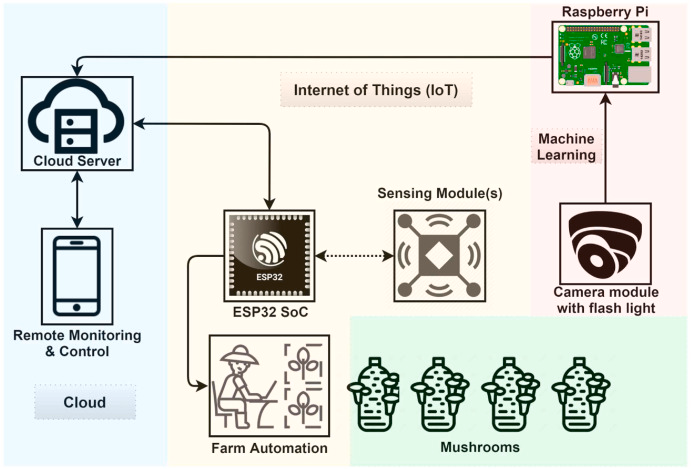
\includegraphics[width=0.5\linewidth]{images/system-example.png}
    \caption{Hệ thống mẫu trong theo dõi và chăm sóc nấm \cite{RAHMAN2022100267}}
    \label{fig:system-example}
\end{figure}

\subsection{Giám sát môi trường}

Việc trồng nấm ăn yêu cầu môi trường đặc biệt và ổn định để có thể sinh trưởng và phát triển. Vì vậy, các thiết bị giám sát môi trường trong hệ thống theo dõi và chăm sóc nấm cần đáp ứng một số đặc điểm và yêu cầu cơ bản để thu thập dữ liệu môi trường một cách chính xác và đáng tin cậy.

\subsubsection{Độ chính xác}
Thiết bị cần có độ chính xác cao trong việc đo lường các thông số môi trường như nhiệt độ, độ ẩm, ánh sáng và các thông số khác. Điều này đảm bảo rằng dữ liệu thu thập được là đáng tin cậy và chính xác để phân tích và đưa ra quyết định.
\subsubsection{Độ phủ}
Thiết bị giám sát môi trường cần có khả năng đo lường và giám sát một phạm vi rộng của môi trường nấm. Ví dụ, trong trường hợp của nấm, cần đo lường nhiệt độ và độ ẩm của không khí, độ ẩm và chất lượng đất, cường độ ánh sáng và các yếu tố khác có thể ảnh hưởng đến sự phát triển và sinh trưởng của nấm.
\subsubsection{Khả năng kết nối}
Thiết bị cần có khả năng giao tiếp và kết nối chia sẻ thông tin với hệ thống giám sát trung tâm để có thể phân tích dữ liệu và đưa ra quyết định tự động tương ứng.
\subsubsection{Hoạt động trong môi trường khắc nghiệt}
Thiết bị cần được thiết kế để chịu được điều kiện môi trường khắc nghiệt trong môi trường nấm. Nó cần có khả năng chống thời tiết, chống bụi, chống ẩm và chịu được nhiệt độ và độ ẩm biến đổi.

\subsection{Điều khiển và tự động hóa}
Trong trồng và chăm sóc nấm, điều khiển và tự động hóa có thể áp dụng để giám sát và điều chỉnh môi trường, tưới nước, chiếu sáng và các hoạt động khác đối với nấm:

\subsubsection{Điều khiển môi trường}

Hệ thống có thể được lập trình để tự động điều chỉnh nhiệt độ, độ ẩm và cường độ ánh sáng trong môi trường nấm. Cảm biến đo lường các thông số này và truyền dữ liệu đến hệ thống điều khiển, từ đó hệ thống điều khiển sẽ thực hiện các điều chỉnh cần thiết để tạo ra môi trường lý tưởng cho sự phát triển của nấm. Ví dụ, nếu nhiệt độ quá cao, hệ thống có thể kích hoạt hệ thống làm mát để giảm nhiệt độ.

Hệ thống tưới nước tự động có thể được sử dụng để cung cấp lượng nước cần thiết cho nấm một cách tự động và chính xác. Cảm biến đo lường độ ẩm đất và truyền dữ liệu đến hệ thống điều khiển. Hệ thống điều khiển có thể tự động kích hoạt hệ thống tưới nước để cung cấp nước khi độ ẩm đất thấp, và ngược lại, ngừng tưới nước khi độ ẩm đạt mức đủ.

Nấm có yêu cầu về ánh sáng để phát triển. Hệ thống điều khiển và tự động hóa có thể được sử dụng để điều chỉnh cường độ và thời gian chiếu sáng. Ví dụ, hệ thống có thể kích hoạt đèn chiếu sáng tự động để cung cấp ánh sáng cho nấm trong các khoảng thời gian nhất định hoặc điều chỉnh cường độ ánh sáng theo yêu cầu của nấm.

\subsubsection{Tự động hóa quy trình}
Hệ thống điều khiển và tự động hóa cũng có thể được sử dụng để tự động hóa các quy trình trồng và chăm sóc nấm. Ví dụ, hệ thống có thể tự động kích hoạt quy trình lấy mẫu nấm, kiểm tra chất lượng không khí, điều chỉnh môi trường, thu hoạch và các hoạt động khác.
    
\subsection{Hệ thống giám sát và phân tích}

Hệ thống giám sát và phân tích tập trung là một hệ thống được sử dụng để thu thập, theo dõi và phân tích dữ liệu từ nhiều nguồn khác nhau một cách tập trung và tổ chức. Nó cung cấp khả năng giám sát và phân tích thông tin từ các thiết bị, hệ thống và quy trình khác nhau trong một tổ chức hoặc môi trường cụ thể. Nhìn chung, hệ thống cần cung cấp khả năng giám sát và kiểm soát toàn diện, phân tích dữ liệu để tìm ra thôngtin hữu ích và hỗ trợ quyết định, và tăng cường khả năng quản lý và tối ưu hóa hoạt động của tổ chức.

\subsubsection{Thu thập dữ liệu}
Hệ thống thu thập dữ liệu từ nhiều nguồn khác nhau như cảm biến, thiết bị đo lường, hệ thống máy tính, máy móc và các nguồn dữ liệu khác. Dữ liệu này có thể bao gồm thông tin về nhiệt độ, độ ẩm, áp suất, lưu lượng, tình trạng thiết bị, dữ liệu về sản xuất và các thông số quan trọng khác.

\subsubsection{Truyền dẫn dữ liệu}
Dữ liệu được truyền từ các nguồn đến hệ thống giám sát và phân tích tập trung thông qua các kết nối mạng, giao thức truyền thông và giao thức liên kết dữ liệu khác nhau. Điều này có thể bao gồm mạng có dây, mạng không dây, giao thức Internet, giao thức truyền thông Modbus và nhiều giao thức khác.

\subsubsection{Lưu trữ và quản lý dữ liệu}
Dữ liệu được lưu trữ và quản lý trong hệ thống giám sát và phân tích tập trung. Hệ thống này thường có cơ sở dữ liệu hoặc hệ thống lưu trữ dữ liệu để lưu trữ và duy trì thông tin thu thập được. Dữ liệu có thể được lưu trữ trong thời gian thực và được cập nhật liên tục để cho phép quá trình giám sát và phân tích liên tục.

\subsubsection{Phân tích và xử lý dữ liệu}
Hệ thống giám sát và phân tích tập trung cung cấp các công cụ và phương pháp để phân tích và xử lý dữ liệu thu thập được. Điều này có thể bao gồm các thuật toán phân tích dữ liệu, công cụ học máy, công cụ thống kê và các phương pháp khác để tìm kiếm thông tin ý nghĩa từ dữ liệu và tạo ra báo cáo, biểu đồ và thông tin hữu ích khác.

\subsubsection{Giao diện người dùng và báo cáo}
Hệ thống giám sát và phân tích tập trung thường cung cấp giao diện người dùng để người dùng có thể truy cập và tương tác với dữ liệu và thông tin. Giao diện này có thể cung cấp các báo cáo, đồ thị, biểu đồ và thông tin trực quan khác để hiển thị dữ liệu và kết quả phân tích một cách dễ hiểu và tiện lợi.

\subsection{Khả năng tích hợp và mở rộng}
Khả năng tích hợp và mở rộng là hai yếu tố quan trọng khi xây dựng hệ thống giám sát và phân tích tập trung. Dưới đây là mô tả về hai khả năng này:

\subsubsection{Khả năng tích hợp}
Khả năng tích hợp đề cập đến khả năng kết nối và làm việc cùng nhau của các thành phần và hệ thống khác nhau. Trong hệ thống giám sát và phân tích tập trung, khả năng tích hợp cho phép các nguồn dữ liệu đa dạng từ các nguồn khác nhau, như cảm biến, thiết bị đo lường, hệ thống máy tính, và các hệ thống hỗ trợ khác, được kết nối và tích hợp vào một hệ thống duy nhất.

Việc có khả năng tích hợp cho phép dữ liệu từ các nguồn khác nhau được thu thập một cách đồng bộ và hiệu quả. Nó cũng giúp tạo ra một cái nhìn toàn diện và đồng nhất về dữ liệu và thông tin trong hệ thống giám sát và phân tích. Các giao thức và tiêu chuẩn quan trọng như MQTT, OPC-UA và RESTful API thường được sử dụng để đảm bảo tích hợp dữ liệu hiệu quả giữa các thành phần khác nhau trong hệ thống.

\subsubsection{Khả năng mở rộng}
Khả năng mở rộng đề cập đến khả năng mở rộng và mở rộng hệ thống giám sát và phân tích tập trung để đáp ứng nhu cầu tăng cường và mở rộng trong tương lai. Điều này bao gồm khả năng thêm mới các thiết bị, cảm biến, hệ thống và nguồn dữ liệu mới vào hệ thống một cách linh hoạt và dễ dàng.

Hệ thống giám sát và phân tích tập trung có thể được mở rộng theo hai hướng: mở rộng theo quy mô và mở rộng chức năng. Mở rộng theo quy mô liên quan đến việc gia tăng khả năng xử lý dữ liệu và lưu trữ để đáp ứng với số lượng nguồn dữ liệu lớn hơn và sự tăng trưởng của hệ thống. Mở rộng chức năng liên quan đến việc thêm mới các chức năng và tính năng mới vào hệ thống để đáp ứng với các yêu cầu và nhu cầu cụ thể.

Các kiến trúc và công nghệ như kiến trúc dựa trên dịch vụ (Service-Oriented Architecture - SOA), kiến trúc dựa trên microservices và sử dụng các công nghệ linh hoạt như điện toán đám mây (cloud computing) và ảo hóa (virtualization) có thể giúp tăng cường khả năng mở rộng của hệ thống giám sát và phân tích tập trung.

\subsection{Quản lý dữ liệu và bảo mật}
Quản lý dữ liệu và bảo mật là hai khía cạnh quan trọng trong hệ thống giám sát và phân tích tập trung. Quản lý dữ liệu đảm bảo tính toàn vẹn, tổ chức, và truy xuất dữ liệu hiệu quả, trong khi bảo mật đảm bảo rằng dữ liệu được bảo vệ khỏi các mối đe dọa an ninh và tuân thủ các quy định liên quan.

\subsubsection{Quản lý dữ liệu}
    
Quản lý dữ liệu trong hệ thống giám sát và phân tích tập trung bao gồm việc thu thập, lưu trữ, xử lý, và truy xuất dữ liệu một cách hiệu quả và có tổ chức. Các nguyên tắc quản lý dữ liệu bao gồm:

\begin{itemize}
    \item Thu thập dữ liệu: Hệ thống phải có khả năng thu thập dữ liệu từ các nguồn khác nhau và đảm bảo tính toàn vẹn và chính xác của dữ liệu thu thập được.
    \item Lưu trữ dữ liệu: Dữ liệu thu thập được cần được lưu trữ một cách an toàn và có tổ chức. Các cơ sở dữ liệu hoặc hệ thống lưu trữ dữ liệu phải được thiết kế để đảm bảo tính bền vững, khả năng mở rộng và khả năng sao lưu/phục hồi dữ liệu.
    \item Xử lý dữ liệu: Dữ liệu thu thập được cần được xử lý để tìm ra thông tin hữu ích và tạo ra các báo cáo, đồ thị, hoặc biểu đồ. Các phương pháp và công cụ phân tích dữ liệu, như học máy, thống kê, và khai phá dữ liệu, có thể được áp dụng để khai thác thông tin từ dữ liệu.
    \item Truy xuất dữ liệu: Hệ thống cần cung cấp khả năng truy xuất dữ liệu một cách nhanh chóng và dễ dàng. Giao diện người dùng và các công cụ truy xuất dữ liệu phải được thiết kế để người dùng có thể truy cập và tìm kiếm dữ liệu một cách thuận tiện.
\end{itemize}

\subsubsection{Bảo mật}
Bảo mật dữ liệu là một yếu tố quan trọng trong hệ thống giám sát và phân tích tập trung, đặc biệt khi xử lý các dữ liệu nhạy cảm hoặc quan trọng. Các biện pháp bảo mật dữ liệu bao gồm:
\begin{itemize}
    \item Quản lý quyền truy cập: Hệ thống nên áp dụng các cơ chế quản lý quyền truy cập để đảm bảo chỉ những người được ủy quyền mới có thể truy cập và xem dữ liệu nhạy cảm. Điều này có thể bao gồm việc sử dụng các phương thức chứng thực và ủy quyền, quản lý vai trò người dùng, và mã hóa dữ liệu.
    \item Mã hóa dữ liệu: Dữ liệu nhạy cảm có thể được mã hóa để đảm bảo rằng chỉ có người được ủy quyền mới có thể giải mã và truy cập dữ liệu. Các thuật toán mã hóa mạnh và các phương pháp quản lý khóa an toàn nên được sử dụng để bảo vệ dữ liệu.
    \item Giám sát và phát hiện xâm nhập: Hệ thống giám sát và phân tích tập trung nên có khả năng giám sát và phát hiện các hoạt động xâm nhập hoặc bất thường. Các công cụ giám sát an ninh, như hệ thống phát hinhập xâm nhập (Intrusion Detection System - IDS) và hệ thống phân tích hành vi (Behavioral Analytics), có thể được triển khai để phát hiện và cảnh báo về các hành vi đáng ngờ hoặc xâm nhập vào hệ thống.
    \item Sao lưu và phục hồi dữ liệu: Việc thực hiện sao lưu định kỳ và quy trình phục hồi dữ liệu là quan trọng để đảm bảo rằng dữ liệu quan trọng không bị mất đi trong trường hợp sự cố hoặc tấn công.
    \item Tuân thủ quy định: Hệ thống giám sát và phân tích tập trung cần tuân thủ các quy định và quyền riêng tư liên quan đến việc xử lý và bảo mật dữ liệu, chẳng hạn như Quy định chung về bảo vệ dữ liệu chung (GDPR) trong Liên minh châu Âu hoặc các quy định quốc gia tương tự.
\end{itemize}

%\section{Sử dụng công nghệ IOT và tự động hóa trong chăm sóc nấm}

\subsection{Hệ thống cảm biến trong giám sát môi trường}

\subsubsection{Cảm biến DHT11 trong giám sát nhiệt độ, độ ẩm môi trường trồng nấm}

Cảm biến nhiệt độ - độ ẩm DHT11 là một cảm biến kỹ thuật số phổ biến được sử dụng để đo và ghi nhận nhiệt độ và độ ẩm trong môi trường.

Với thông số có độ chính xác vừa phải (Bảng \ref{tab:dht11-specs}), cảm biến DHT11 thường được sử dụng trong các ứng dụng như đo nhiệt độ và độ ẩm trong môi trường, giám sát thời tiết, kiểm soát môi trường nhiệt độ - độ ẩm trong nhà, và các ứng dụng liên quan đến IoT (Internet of Things) và nhà thông minh.

\begin{table}[]
\centering
\caption{Thông số kỹ thuật cảm biến DHT11}
\label{tab:dht11-specs}
\begin{tabular}{|l|l|}
\hline
\multicolumn{1}{|c|}{\textbf{Thông số kỹ thuật}} & \multicolumn{1}{c|}{\textbf{Giá trị}} \\ \hline
Phạm vi đo nhiệt độ                              & 0°C đến 50°C                          \\ \hline
Phạm vi đo độ ẩm                                 & 20\% đến 90\%                         \\ \hline
Độ chính xác nhiệt độ                            & ± 2°C                                 \\ \hline
Độ chính xác độ ẩm                               & ± 5\%                                 \\ \hline
Độ phân giải nhiệt độ                            & 0.1°C                                 \\ \hline
Độ phân giải độ ẩm                               & 1\%                                   \\ \hline
Điện áp hoạt động                                & 3.3V - 5V DC                          \\ \hline
Dòng tiêu thụ                                    & 1-2mA                                 \\ \hline
Giao tiếp                                        & Giao tiếp 1 dây, nhị phân             \\ \hline
Tốc độ truyền dữ liệu                            & Tối đa 1Hz (1 giây/lần)               \\ \hline
Kích thước                                       & 15.5mm x 12mm x 5.5mm                 \\ \hline
\end{tabular}
\end{table}

\subsubsection{Sử dụng Camera IP cho theo dõi và giám sát nấm}

Camera IP được sử dụng trong giám sát hình ảnh là một thiết bị mạng có khả năng ghi lại và truyền hình ảnh và âm thanh qua mạng IP. Nó cho phép người dùng từ xa quan sát và quản lý hình ảnh từ các vị trí khác nhau thông qua kết nối mạng.

Định dạng MJPEG (Motion JPEG) là một định dạng nén hình ảnh chuyển động sử dụng rộng rãi trong Camera IP. Nó sử dụng một chuỗi các khung hình JPEG độc lập để tạo ra video. Mỗi khung hình trong chuỗi MJPEG là một hình ảnh độc lập và không phụ thuộc vào các khung hình trước và sau đó. Điều này có nghĩa là mỗi khung hình có thể được giải nén và xem một cách độc lập.

Ưu điểm của định dạng MJPEG bao gồm:
\begin{itemize}
    \item Chất lượng hình ảnh tốt: MJPEG giữ được chất lượng hình ảnh cao trong mỗi khung hình do sử dụng nén JPEG độc lập cho từng khung hình.
    \item Khả năng xử lý đơn giản: Vì mỗi khung hình là độc lập, việc xử lý và truyền tải video MJPEG đơn giản hơn so với các định dạng video khác như H.264 hoặc MPEG.
    \item Khả năng tái sử dụng khung hình: Với MJPEG, các khung hình có thể dễ dàng được trích xuất và lưu trữ từ video, việc này hữu ích trong việc xem xét các sự kiện quan trọng hoặc tạo ảnh chụp nhanh từ video.
\end{itemize}

Tuy nhiên, định dạng MJPEG cũng có một số hạn chế:
\begin{itemize}
    \item Kích thước tập tin lớn: MJPEG có xu hướng tạo ra các tập tin video lớn hơn so với các định dạng nén video khác như H.264 hoặc MPEG, do mỗi khung hình được nén riêng lẻ.
    \item Băng thông mạng cao: Do kích thước tập tin lớn, việc truyền tải video MJPEG qua mạng yêu cầu băng thông cao hơn so với các định dạng video nén khác.
    \item Khả năng lưu trữ: Vì kích thước tập tin lớn, việc lưu trữ video MJPEG yêu cầu nhiều dung lượng lưu trữ hơn so với các định dạng video nén khác.
\end{itemize}

Với những ưu điểm như vậy, MJPEG là một định dạng phổ biến được sử dụng trong camera IP để giám sát hình ảnh. Đối với hệ thống giám sát sinh trưởng của nấm, nấm sinh trưởng trong thời gian dài nên hình ảnh thu nhận không yêu cầu liên tục. Như vậy, dữ liệu lưu trữ cũng không chiếm nhiều dung lượng do hình ảnh được lưu trữ rời rạc.

\subsection{Điều chỉnh điều kiện môi trường trồng nấm}

\subsection{Thiết bị giám sát và điều khiển trung tâm sử dụng Raspberry Pi 3}

Raspberry Pi 3 là một máy tính nhỏ gọn với khả năng xử lý mạnh mẽ và khả năng kết nối mạng tích hợp. Nó được sử dụng rộng rãi trong các dự án IoT, hệ thống nhúng và các ứng dụng máy tính nhỏ gọn. Với CPU Quad-Core và RAM 1GB, Raspberry Pi 3 có thể chạy các ứng dụng đa nhiệm và xử lý đa phương tiện.

Raspberry Pi 3 sử dụng khe cắm thẻ microSD để lưu trữ hệ điều hành và dữ liệu. Đối với nhu cầu lưu trữ lớn hơn và hiệu suất cao hơn, Raspberry Pi 3 cũng hỗ trợ kết nối các thiết bị lưu trữ ngoại vi như ổ cứng USB hoặc ổ SSD thông qua các cổng USB. Bằng cách kết nối một thiết bị lưu trữ ngoại vi, có thể mở rộng không gian lưu trữ và tận dụng tốc độ truyền dữ liệu nhanh hơn so với thẻ microSD (Bảng \ref{tab:rpi3-specs}.

\begin{table}[h]
\centering
\caption{Thông số kỹ thuật Raspberry Pi 3}
\label{tab:rpi3-specs}
\begin{tabular}{|l|l|}
\hline
\multicolumn{1}{|c|}{\textbf{Thông số kỹ thuật}} & \multicolumn{1}{c|}{\textbf{Giá trị}}                                                                           \\ \hline
CPU                                              & \begin{tabular}[c]{@{}l@{}}Broadcom BCM2837 64-bit Quad-Core ARM\\  Cortex-A53\end{tabular}                     \\ \hline
Tốc độ CPU                                       & 1.2 GHz                                                                                                         \\ \hline
RAM                                              & 1 GB LPDDR2 SDRAM                                                                                               \\ \hline
Kết nối mạng                                     & 10/100 Ethernet, Wi-Fi 802.11n, Bluetooth 4.2                                                                   \\ \hline
Giao diện                                        & \begin{tabular}[c]{@{}l@{}}4 cổng USB 2.0, HDMI, Ethernet, jack 3.5mm,\\Camera CSI, Display DSI\end{tabular}  \\ \hline
Đồ họa                                           & VideoCore IV 3D                                                                                                 \\ \hline
Lưu trữ                                          & Khe cắm thẻ microSD                                                                                             \\ \hline
Hệ điều hành hỗ trợ                              & \begin{tabular}[c]{@{}l@{}}Raspbian, Ubuntu, Windows 10 IoT Core\\  và các hệ điều hành Linux khác\end{tabular} \\ \hline
Kích thước                                       & 85mm x 56mm x 17mm                                                                                              \\ \hline
Nguồn điện                                       & 5V DC qua cổng micro USB                                                                                        \\ \hline
\end{tabular}
\end{table}

Raspberry Pi 3 cung cấp các giao diện và kết nối phổ biến để kết nối camera, thiết bị điều khiển và cảm biến. Dưới đây là một số phương pháp kết nối thông qua các giao diện của Raspberry Pi 3:

\subsubsection{Kết nối Camera}
Raspberry Pi 3 hỗ trợ kết nối camera thông qua giao diện Camera Serial Interface (CSI). Giao diện CSI có thể được sử dụng để kết nối các module camera tương thích với Raspberry Pi, cho phép bạn ghi lại hình ảnh hoặc thực hiện xử lý hình ảnh trực tiếp trên Pi.

\subsubsection{Kết nối Thiết bị điều khiển}
Raspberry Pi 3 hỗ trợ kết nối và điều khiển các thiết bị ngoại vi thông qua các giao diện như GPIO (General Purpose Input/Output). Các chân GPIO trên Raspberry Pi 3 cho phép người dùng kết nối và điều khiển các thiết bị như bàn phím, chuột, nút nhấn, LED, servo motor và nhiều thiết bị điều khiển khác.

\subsubsection{Kết nối Cảm biến}
Raspberry Pi 3 có thể kết nối với nhiều loại cảm biến thông qua các giao diện như GPIO và giao thức I2C. Giao diện GPIO cho phép bạn kết nối các cảm biến analog hoặc digital trực tiếp vào Raspberry Pi 3. Giao thức I2C cung cấp khả năng kết nối nhiều cảm biến thông qua một dây dẫn, giúp tiết kiệm chân kết nối.

Ngoài ra, Raspberry Pi 3 cũng hỗ trợ các giao diện khác như USB, SPI và UART cho phép kết nối và giao tiếp với các thiết bị ngoại vi khác như camera, mô đun giao tiếp không dây và các thiết bị khác.

\section{Ứng dụng công nghệ thị giác máy tính trong theo dõi và chăm sóc nấm}

\subsection{Lợi ích của công nghệ thị giác máy tính}

Ứng dụng thị giác máy tính trong trồng và theo dõi nấm có thể mang lại nhiều lợi ích quan trọng, bao gồm:

\begin{itemize}
    \item Phân loại và nhận dạng loại nấm: Thị giác máy tính có thể được sử dụng để phân loại và nhận dạng các loại nấm khác nhau. Bằng cách sử dụng các thuật toán nhận dạng hình ảnh và mô hình học máy, có thể xây dựng các hệ thống tự động phân loại nấm dựa trên hình ảnh. Điều này giúp cho việc xác định loại nấm trở nên nhanh chóng và chính xác hơn, giúp cho việc trồng và quản lý nấm hiệu quả hơn.
    \item Đếm và theo dõi sự phát triển của nấm: Thị giác máy tính có thể được sử dụng để đếm và theo dõi sự phát triển của nấm trong quá trình trồng. Bằng cách phân tích hình ảnh và xử lý dữ liệu, có thể xác định số lượng nấm, kích thước và tốc độ phát triển của chúng. Điều này giúp cho việc quản lý và điều chỉnh điều kiện trồng nấm một cách chính xác, đảm bảo sự phát triển và sản xuất nấm tốt nhất.
    \item Phát hiện bệnh và xác định tình trạng sức khỏe của nấm: Thị giác máy tính có thể được sử dụng để phát hiện các bệnh và xác định tình trạng sức khỏe của nấm. Bằng cách phân tích hình ảnh và so sánh với các mẫu dữ liệu đã biết, có thể phát hiện các dấu hiệu của bệnh hoặc tình trạng không tốt trong nấm. Điều này giúp cho việc phát hiện sớm các vấn đề và triển khai biện pháp can thiệp kịp thời để ngăn chặn sự lây lan và tổn thất nấm.
    \item Đánh giá chất lượng và thu hoạch: Thị giác máy tính có thể được sử dụng để đánh giá chất lượng của nấm và hỗ trợ trong quá trình thu hoạch. Bằng cách phân tích hình ảnh và áp dụng các tiêu chí chất lượng đã được định nghĩa trước, có thể đánh giá và phân loại nấm dựa trên kích thước, hình dạng, màu sắc và các đặc điểm khác. Điều này giúp cho việc tạo ra sản phẩm nấm có chất lượng cao và đáp ứng yêu cầu của thị trường.
\end{itemize}


\subsection{Mô hình CNN và vai trò của CNN trong phát hiện và phân loại ảnh}

\acrfull{cnn} là một loại mô hình học sâu được sử dụng rộng rãi trong xử lý hình ảnh và thị giác máy tính. Nó được thiết kế đặc biệt để hiệu quả trong việc xử lý thông tin không gian và bao gồm các lớp tích chập và lớp gộp để trích xuất các đặc trưng từ hình ảnh.

\acrshort{cnn} có thể được sử dụng trong việc phát hiện và phân loại nấm:

\subsubsection{Phát hiện nấm}
\acrshort{cnn} có thể được sử dụng để phát hiện sự hiện diện của nấm trong hình ảnh. Bằng cách huấn luyện mô hình \acrshort{cnn} với các tập dữ liệu chứa hình ảnh nấm và không nấm, nó có thể học cách nhận diện các đặc trưng đặc biệt của nấm. Khi áp dụng mô hình này vào hình ảnh mới, nó có thể xác định xem có nấm xuất hiện hay không. Điều này có thể hữu ích trong việc đánh giá sự hiện diện nấm trong môi trường trồng hoặc trong các ứng dụng quan trọng như phát hiện nấm độc hại trong thực phẩm hoặc trong tự nhiên.

\subsubsection{Phân tích sự phát triển và tình trạng sức khỏe}
\acrshort{cnn} có thể được sử dụng để phân tích sự phát triển và tình trạng sức khỏe của nấm dựa trên hình ảnh. Bằng cách huấn luyện mô hình \acrshort{cnn} với các tập dữ liệu chứa hình ảnh của nấm ở các giai đoạn phát triển khác nhau hoặc ở các tình trạng sức khỏe khác nhau, nó có thể học cách nhận diện các đặc trưng liên quan. Khi áp dụng mô hình này vào hình ảnh mới, nó có thể đánh giá sự phát triển và tình trạng sức khỏe của nấm dựa trên các đặc trưng đã học được, giúp cho việc theo dõi và quản lý nấm trong quá trình trồng.

\subsection{Mô hình YOLO và ưu điểm của YOLO trong phát hiện vật thể}

\acrfull{yolo} là một thuật toán phát hiện đối tượng có một số ưu điểm so với các phương pháp phát hiện đối tượng dựa trên \acrshort{cnn} truyền thống. Dưới đây là một số ưu điểm của \acrfull{yolo} so với \acrshort{cnn}:

\begin{itemize}
    \item Tốc độ: YOLO được biết đến với tốc độ suy đoán nhanh. Khác với các phương pháp phát hiện đối tượng dựa trên CNN truyền thống yêu cầu nhiều lần chạy qua các lớp ảnh hoặc cửa sổ trượt, YOLO thực hiện phát hiện đối tượng trong một lần chạy duy nhất. Điều này làm cho YOLO nhanh hơn đáng kể và hiệu quả hơn trong việc xử lý ảnh thời gian thực.
    \item Độ chính xác và đồng nhất: YOLO tạo ra các dự đoán đối tượng trực tiếp trên một lưới ô mà không cần phải xem xét các vùng đặc trưng. Điều này dẫn đến độ chính xác cao và sự đồng nhất trong việc phát hiện đối tượng. So với các phương pháp truyền thống, YOLO thường có khả năng phát hiện đối tượng nhỏ và đa dạng tốt hơn.
    \item Khả năng phát hiện đa đối tượng: YOLO có khả năng phát hiện và phân loại nhiều đối tượng trong một lần chạy. Nó có thể xác định và định vị các đối tượng không đối xứng trên cùng một hình ảnh một cách hiệu quả. Điều này làm cho YOLO phù hợp trong các ứng dụng yêu cầu phát hiện nhanh chóng và đồng thời của nhiều đối tượng.
    \item Kiến trúc đơn giản: YOLO có cấu trúc kiến trúc đơn giản và dễ hiểu. Nó bao gồm một mạng neural duy nhất và không yêu cầu quá trình rời rạc như làm việc với các cửa sổ trượt. Do đó, việc triển khai và huấn luyện YOLO trở nên đơn giản và tiện lợi.
\end{itemize}

\section{Tổng kết chương}

Chương 1 của báo cáo tập trung vào việc tìm hiểu về sản xuất nấm ăn tại Việt Nam và những thách thức mà ngành này đang phải đối mặt. Nấm được coi là loại thực phẩm có ý nghĩa và giá trị kinh tế quan trọng, tuy nhiên, sản xuất nấm truyền thống đang gặp phải nhiều khó khăn.

Chương cũng nêu rõ sự phát triển của công nghệ IoT (Internet of Things) và tự động hóa trong nông nghiệp, đặc biệt là trong sản xuất nấm. Các công nghệ này mang lại nhiều tiện ích và cơ hội mới cho ngành sản xuất nấm.

Để xây dựng hệ thống theo dõi và chăm sóc nấm hiệu quả, chương cung cấp các đặc điểm yêu cầu của hệ thống, bao gồm giám sát môi trường, điều khiển và tự động hóa, hệ thống giám sát và phân tích, khả năng tích hợp và mở rộng, quản lý dữ liệu và bảo mật.

Công nghệ IoT và tự động hóa được đề xuất và áp dụng trong chăm sóc nấm. Chương trình nêu rõ việc sử dụng hệ thống cảm biến để giám sát môi trường trồng nấm và điều chỉnh điều kiện môi trường. Ngoài ra, chương trình cũng giới thiệu thiết bị giám sát và điều khiển trung tâm sử dụng Raspberry Pi 3.

Cuối cùng, chương cung cấp một cái nhìn tổng quan về ứng dụng của công nghệ thị giác máy tính trong việc theo dõi và chăm sóc nấm. Các mô hình CNN (Convolutional Neural Network) và YOLO (You Only Look Once) được giới thiệu và giải thích vai trò của chúng trong phát hiện và phân loại ảnh.

Chương 1 giúp định hình nền tảng cho việc nghiên cứu và triển khai các hệ thống theo dõi và chăm sóc nấm sử dụng các công nghệ IoT, tự động hóa và thị giác máy tính.
% !TeX root = ../main.tex

\chapter{CƠ SỞ LÝ THUYẾT VỀ MẠNG NƠ-RON TÍCH CHẬP VÀ MÔ HÌNH YOLO}

\section{Mạng nơ-ron tích chập trong thị giác máy tính}

Mạng nơ ron tích chập (Convolutional Neural Network - CNN) là một kiến trúc mạng nơ ron được sử dụng phổ biến trong lĩnh vực xử lý ảnh và nhận dạng đối tượng. Đặc điểm chính của CNN bao gồm:

\begin{itemize}
	\item Lớp tích chập (Convolutional Layer): Là lớp cốt lõi của CNN, sử dụng phép tích chập để trích xuất đặc trưng từ ảnh đầu vào. Lớp này sử dụng các bộ lọc (filter) để thực hiện phép tích chập trên ảnh và tạo ra các feature map, trong đó mỗi pixel của feature map biểu diễn mức độ kích hoạt của một đặc trưng cụ thể.
	\item Lớp gộp (Pooling Layer): Được sử dụng để giảm kích thước của feature map và giảm số lượng tham số trong mạng. Lớp gộp thường áp dụng các phép tổng hợp như lấy giá trị lớn nhất (Max Pooling) hoặc lấy giá trị trung bình (Average Pooling) trong một vùng nhất định trên feature map.
	\item Lớp kích hoạt (Activation Layer): Áp dụng một hàm kích hoạt phi tuyến (như ReLU - Rectified Linear Unit) sau lớp tích chập để tạo độ không tuyến tính và giúp mô hình học được các đặc trưng phức tạp hơn.
	\item Lớp kết nối đầy đủ (Fully Connected Layer): Là một loại lớp nơ ron truyền thống, kết nối các đặc trưng đã được trích xuất từ lớp trước với các nơ ron trong lớp này. Lớp này thường xuất ra các đầu ra cuối cùng của mạng, thường là các xác suất phân loại của các lớp đối tượng.
	\item Hàm mất mát (Loss Function): Được sử dụng để đánh giá sự khác biệt giữa kết quả dự đoán và giá trị thực tế. Các hàm mất mát phổ biến trong CNN bao gồm hàm Cross-Entropy và hàm Mean Squared Error.
	\item Tính chia sẻ tham số (Parameter Sharing): CNN sử dụng cơ chế chia sẻ tham số giữa các vùng không gian trong ảnh để giảm số lượng tham số cần học. Thay vì học các trọng số riêng cho mỗi vùng của ảnh, CNN chia sẻ các trọng số giữa các vùng có cùng đặc trưng.
	\item Kiến trúc kiểu "tầng" (Layered Architecture): CNN được tổ chức thành một chuỗi các lớp xếp chồng lên nhau, mỗi lớp đóng vai trò trong việc trích xuất và học các đặc trưng từ dữ liệu. Kiến trúc kiểu "tầng" giúp mạng học được các đặc trưng từ cấp thấp đến cấp cao, từ các nét cơ bản đến các đặc trưng phức tạp hơn.
\end{itemize}

\begin{figure}
	\centering
	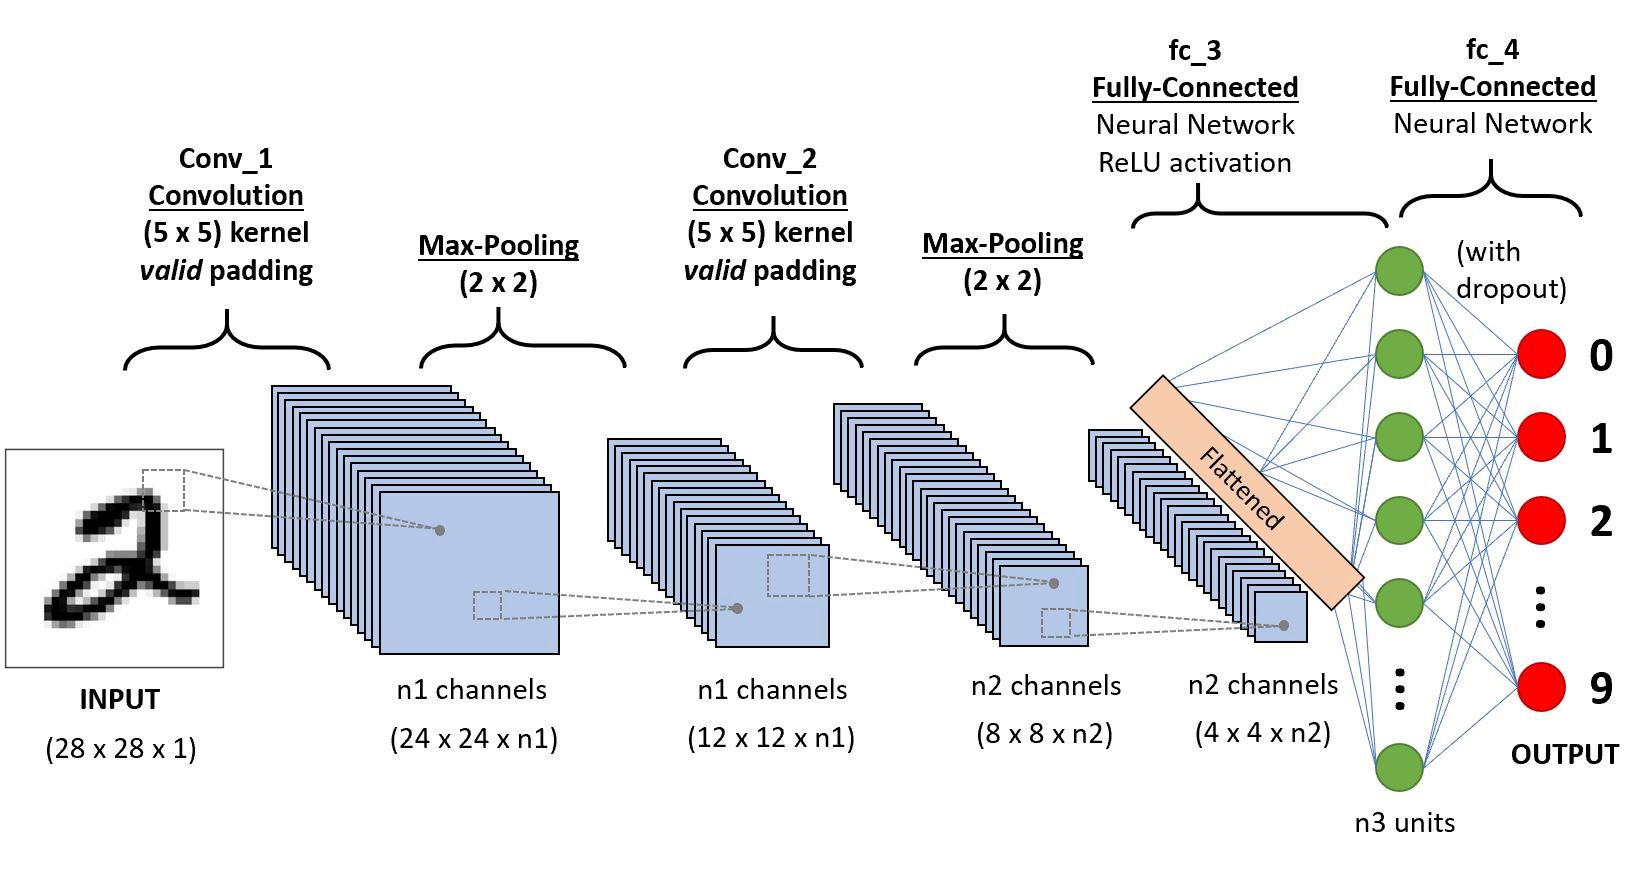
\includegraphics[width=0.9\linewidth]{images/typical-cnn.png}
	\caption{Mạng nơ-ron tích chập điển hình\cite{Ratan_2023}}
	\label{fig:typical-cnn}
\end{figure}

Tổng quan, mạng nơ ron tích chập là một kiến trúc mạng nơ ron đặc biệt được thiết kế để xử lý và trích xuất đặc trưng từ dữ liệu ảnh. Các đặc điểm của CNN như lớp tích chập, lớp gộp, lớp kích hoạt, lớp kết nối đầy đủ và tính chia sẻ tham số giúp cho CNN có khả năng học và trích xuất các đặc trưng từ dữ liệu ảnh một cách hiệu quả. Kiến trúc kiểu "tầng" trong CNN cho phép mạng học được các đặc trưng từ cấp thấp đến cấp cao, từ các nét cơ bản đến các đặc trưng phức tạp hơn.

\subsection{Dữ liệu đầu vào}

Dữ liệu hình ảnh đầu vào cho mạng nơ-ron tích chập (CNN) thường là các bức ảnh được biểu diễn dưới dạng ma trận điểm ảnh. Mỗi điểm ảnh trong ma trận thể hiện mức độ sáng tại mỗi vị trí trên ảnh.

Thông thường các ảnh màu đầu vào sẽ có các kênh màu RGB, trong đó mỗi kênh màu tương ứng với một thành phần màu đỏ (R), xanh lá cây (G) và xanh dương (B). Với mỗi điểm ảnh, giá trị của từng kênh màu (R, G, B) thường được biểu diễn bằng một con số trong khoảng từ 0 đến 255.

Kích thước của ảnh đầu vào có thể khác nhau tùy thuộc vào yêu cầu của bài toán và kiến trúc của mạng CNN. Các kích thước phổ biến cho ảnh đầu vào là 224x224, 256x256, 299x299 hoặc 512x512 điểm ảnh.

Trước khi đưa dữ liệu hình ảnh vào mạng CNN, dữ liệu cần đưa qua một số bước tiền xử lý:

\begin{enumerate}
	\item Chuẩn hóa: Để đảm bảo rằng các giá trị pixel trong ảnh nằm trong khoảng từ 0 đến 1. Như vậy cần phải chuẩn hóa dữ liệu bằng cách chia tất cả các giá trị điểm ảnh cho 255 đối với kiểu dữ liệu 8 bít hoặc chia cho $2^n-1$ với $n$ là kích thước số nguyên của điểm ảnh.
	\item Thay đổi kích thước: Nếu kích thước của ảnh không phù hợp với kích thước đầu vào của mạng CNN, cần thực hiện điều chỉnh kích thước ảnh để phù hợp. Thông thường, sử dụng phép thay đổi tuyến tính hoặc cắt ảnh để thay đổi kích thước ảnh.
	\item Tăng cường dữ liệu huấn luyện: Đối với các bài toán mạng CNN, việc sử dụng kỹ thuật tăng cường dữ liệu khi huấn luyện có thể giúp tăng tính tổng quát hóa của mô hình. Tăng cường dữ liệu bao gồm việc áp dụng các phép biến đổi như xoay, lật, phóng to, thu nhỏ, và thay đổi độ sáng để tạo ra các phiên bản mới của dữ liệu hình ảnh.
\end{enumerate}

Dữ liệu trong cnn được biểu diễn dưới dạng ma trận. Dữ liệu hình ảnh đầu vào sẽ được biểu diễn dưới dạng \ref{input_shape}.

\begin{equation}
	\centering
	\label{input_shape}
	(N \times C \times H_{in} \times W_{in})
\end{equation}

Trong đó
\begin{itemize}
	\item $N$ là số hình ảnh đầu vào theo lô.
	\item $C$ là số kênh, ảnh mức xám có số kênh bằng 1, ảnh RGB có số kênh bằng 3.
	\item $H_{in}$ là chiều cao ảnh.
	\item $W_{in}$ là chiều rộng ảnh.
\end{itemize}

\subsection{Lớp tích chập}

\subsubsection{Phép chập}

Phép chập là một phép toán cơ bản trong xử lý ảnh dùng để xác định đặc trưng giữa các điểm ảnh trong một hình ảnh và xây dựng các bộ lọc để trích xuất đặc trưng hay thực hiện các phép biến đổi hình ảnh. Hình \ref{fig:edge-detection-conv} mô tả ứng dụng của phép tích chập trong bài toán phát hiện biên theo chiều dọc.

% TODO: \usepackage{graphicx} required
\begin{figure}[h]
	\centering
	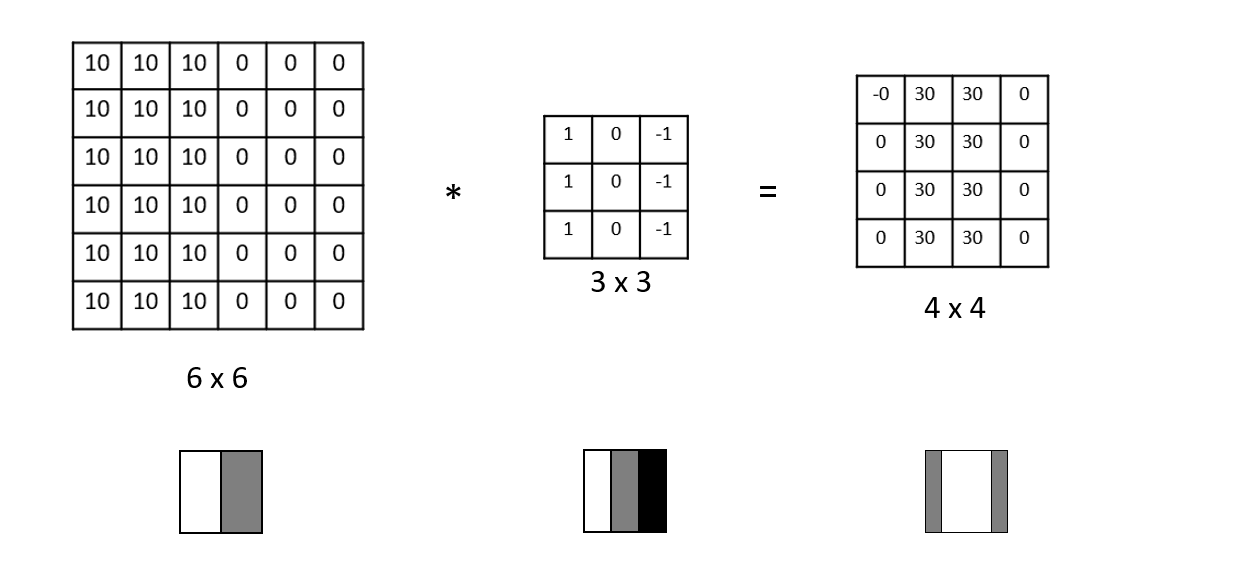
\includegraphics[width=0.8\linewidth]{images/edge-detection-conv}
	\caption{Phép tích chập trong phát hiện dọc}
	\label{fig:edge-detection-conv}
\end{figure}

Kết quả từng vị trí của ma trận ra trong phép chập tính bằng cách tính tổng của tích từng phần tử của bộ lọc với phần tử tại vị trí tương ứng trên ma trận vào. Thực hiện di chuyển bộ lọc tới các vị trí khác nhau để tính toán giá trị các vị trí còn lại. Hình \ref{fig:conv-operation} mô tả quá trình thực hiện chập ma trận vào với bộ lọc để được kết quả phần tử đầu tiên của ma trận ra.

% TODO: \usepackage{graphicx} required
\begin{figure}
	\centering
	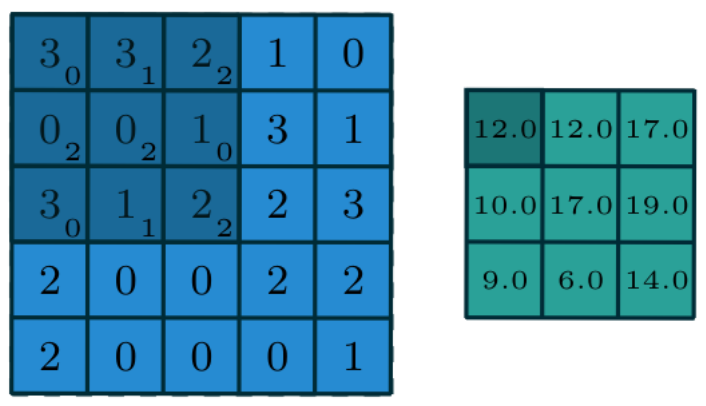
\includegraphics[width=0.6\linewidth]{images/conv-operation}
	\caption{Phép chập}
	\label{fig:conv-operation}
\end{figure}


\subsubsection{Kích thước bộ lọc}

Kích thước bộ lọc $k$ là kích thước của ma trận bộ lọc trong phép tích chập. Trong phần lớn trường hợp, kích thước bộ lọc được sử dụng có dạng vuông, tức chiều rộng bằng chiều cao và bằng $k$. 

Kích thước của bộ lọc có ảnh hưởng đến cách tính toán phép tích chập và kích thước của đầu ra. Khi bộ lọc có kích thước lớn hơn, nó có khả năng nhìn thấy một khu vực lớn hơn trên đầu vào và có thể giúp phát hiện các đặc trưng toàn cục. Tuy nhiên, nó cũng tăng độ phức tạp tính toán và có thể dẫn đến việc mất thông tin chi tiết trong đầu vào. Ngược lại, khi bộ lọc có kích thước nhỏ hơn, nó tập trung vào phát hiện các đặc trưng cục bộ và tạo ra đầu ra có kích thước nhỏ hơn. Các giá trị thông thường cho kích thước bộ lọc là 3\times 3, 5\times 5, 7\times 7.

\subsubsection{Thuộc tính đệm}

Thông thường, khi chập trực tiếp bộ lọc với ma trận vào ta sẽ thu được ma trận ra với kích thước nhỏ hơn (Hình \ref{fig:no-padding-unit-stride}). Do đó,đệm được sử dụng để thay đổi kích thước đầu vào trước khi áp dụng tích chập nhằm thu được đầu ra theo ý muốn.

% TODO: \usepackage{graphicx} required
\begin{figure}[h]
	\centering
	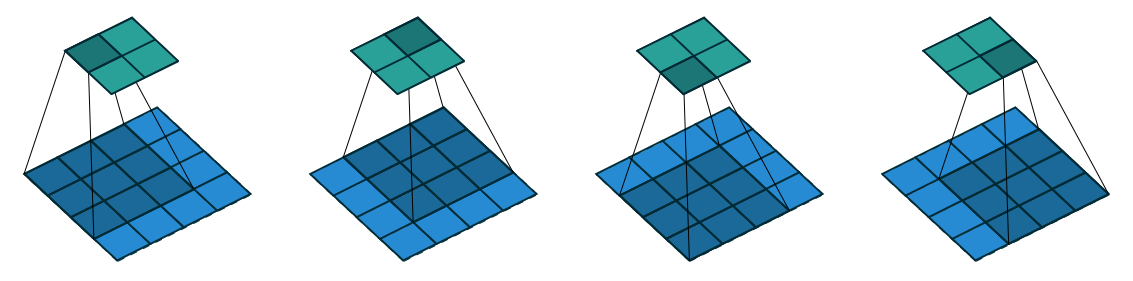
\includegraphics[width=0.9\linewidth]{images/no-padding-unit-stride}
	\caption{Chế độ không đệm, bước nhảy đơn vị}
	\label{fig:no-padding-unit-stride}
\end{figure}

Có 2 loại đệm:
\begin{itemize}
	\item Đệm nửa đảm bảo kích thước ma trận đầu ra bằng kích thước ma trận đầu vào (Hình \ref{fig:half-padding-unit-stride1}). Giá trị đệm nửa xác định bằng công thức \ref{eqn:haft-padding}.
	\begin{equation}\label{eqn:haft-padding}
		p = \frac{k-1}{2}
	\end{equation}
	\item Đệm đầy đủ đảm bảo kích thước ma trận đầu ra lớn hơn hoặc bằng kích thước ma trận đầu vào (Hình \ref{fig:full-padding-unit-stride}). Giá trị đệm đầy đủ tính bằng công thức \ref{eqn:full-padding}.
	\begin{equation}\label{eqn:full-padding}
		p = k-1
	\end{equation}
\end{itemize}
% TODO: \usepackage{graphicx} required
\begin{figure}
	\centering
	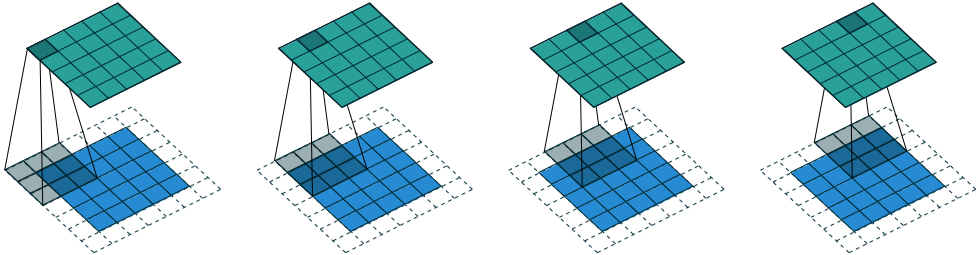
\includegraphics[width=0.9\linewidth]{images/half-padding-unit-stride1}
	\caption{Chế độ đệm nửa, bước nhảy đơn vị}
	\label{fig:half-padding-unit-stride1}
\end{figure}

% TODO: \usepackage{graphicx} required
\begin{figure}
	\centering
	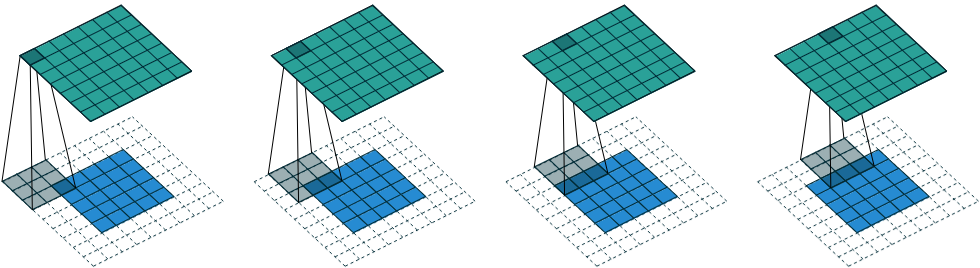
\includegraphics[width=0.9\linewidth]{images/full-padding-unit-stride}
	\caption{Chế độ đệm đầy đủ, bước nhảy đơn vị}
	\label{fig:full-padding-unit-stride}
\end{figure}

\subsubsection{Thuộc tính bước nhảy}

Bước nhảy là số lượng phần tử giữa hai lần áp dụng tích chập ma trận đầu vào với bộ lọc. Như vậy, thay vì di chuyển 1 điểm ảnh trên ảnh đầu vào trong phép tích chập thông thường, áp dụng bước nhảy sẽ di chuyển ma trận với $s$ điểm ảnh (Hình \ref{fig:half-padding-stride-2}).

% TODO: \usepackage{graphicx} required
\begin{figure}[h]
	\centering
	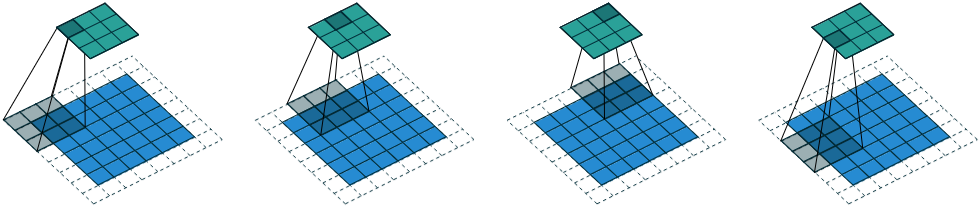
\includegraphics[width=0.9\linewidth]{images/half-padding-stride-2}
	\caption{Chế độ đệm nửa, bước nhảy 2}
	\label{fig:half-padding-stride-2}
\end{figure}

Sử dụng bước nhảy có thể làm giảm kích thước của đầu ra so với đầu vào ban đầu, vì những vị trí không được xem xét. Tuy nhiên, bước nhảy cũng giúp giảm độ phức tạp tính toán và số lượng tham số trong mạng nơ-ron tích chập, đồng thời có thể tạo ra các biểu diễn đặc trưng tổng quát hơn và giảm hiện tượng overfitting.


Việc kết hợp bước nhảy và đệm tạo ra ma trận với kích thước tính theo công thức \ref{eqn:padding-stride}.

\begin{equation}\label{eqn:padding-stride}
	o = \lfloor{\frac{i-k}{s}}\rfloor + 1
\end{equation}

\subsubsection{Phép chập khối}

Trong thực tế, việc áp dụng các bộ lọc trên ảnh thường được áp dụng cho cả 3 kênh màu đỏ, lục và lam. Như vậy, bộ lọc hay khối lọc cần có 3 chiều bao gồm màu sắc, chiều cao và chiều rộng. Hình \ref{fig:single-filter-block-conv} mô tả ảnh đầu vào kích thước $6 \times 6$ trên hệ màu RGB.Như vậy, đầu vào có thể biểu diễn dạng ma trận kích thước $(6 \times 6 \times 3)$. Khối lọc để áp dụng tương ứng cũng phải có 3 lớp tương ứng với 3 màu đỏ, lục và lam.

% TODO: \usepackage{graphicx} required
\begin{figure}[h]
	\centering
	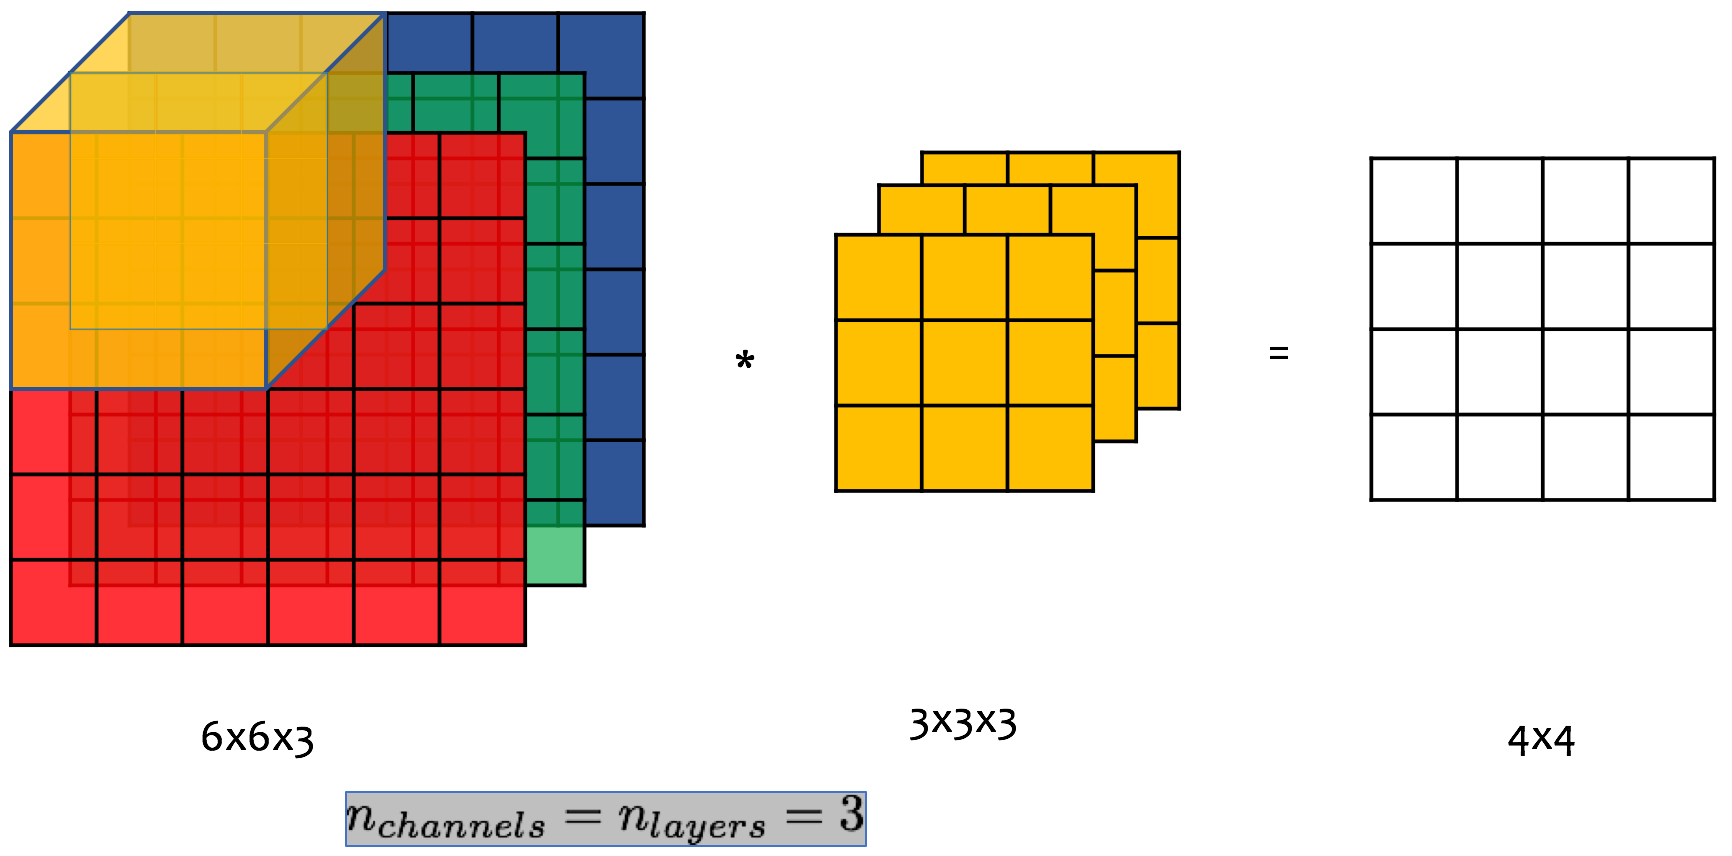
\includegraphics[width=0.8\linewidth]{images/single-filter-block-conv}
	\caption{Phép chập khối \cite{dl_app_2018}}
	\label{fig:single-filter-block-conv}
\end{figure}

Việc tính toán kết quả sau khi áp dụng khối lọc thực hiện bằng cách dịch chuyển khối lọc trên khối ma trận vào. Mỗi lớp của bộ lọc được chập với diện tích phủ bởi nó trên kênh tương ứng của ma trận vào. Tại một vị trí tương ứng của khối lọc, giá trị tại ô tương ứng của ma trận đầu ra là tổng của các kết quả phép chập trên từng lớp.

Phép chập có thể được sử dụng để phát hiện và trích xuất đặc trưng trên một hoặc nhiều kênh vào. Ví dụ, để phát hiện đặc trưng trên kênh màu đỏ và bỏ qua kênh màu xanh lục và xanh lam, bộ phát hiện chỉ được đặt ở lớp đầu tiên và giá trị 2 lớp còn lại bằng 0.

\subsubsection{Phép chập khối với nhiều bộ lọc}

Sau mỗi khối lọc, kết quả thu được sau khi thực hiện chập với ma trận khối đầu vào là một ma trận 2 chiều tương ứng với một đặc trưng của đầu vào. Để thu được nhiều đặc trưng từ ảnh đầu vào, có thể sử $n$ khối lọc lần lượt chập với ma trận đầu vào để thu được $n$ ma trận đầu ra, xếp chồng chúng trở thành $n$ kênh đặc trưng đầu ra (Hình \ref{fig:multiple-filter-block-conv}).

% TODO: \usepackage{graphicx} required
\begin{figure}[h]
	\centering
	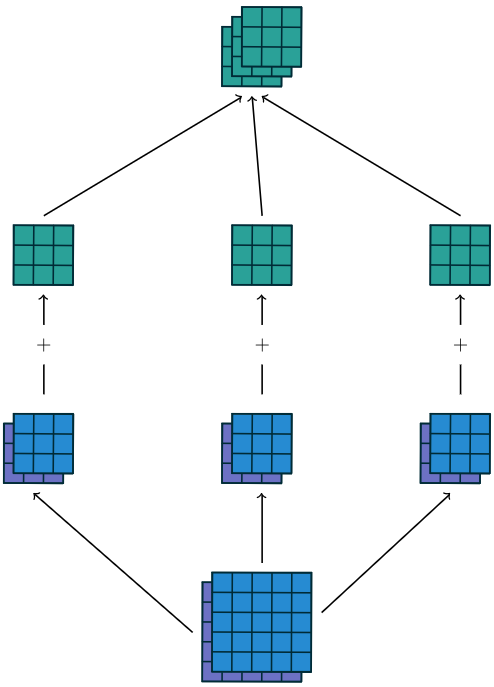
\includegraphics[width=0.6\linewidth]{images/multiple-filter-block-conv}
	\caption{Phép chập nhiều bộ lọc \cite{wei2021}}
	\label{fig:multiple-filter-block-conv}
\end{figure}



\subsection{Lớp gộp}
Lớp gộp là một lớp quan trọng giúp giảm kích thước không gian đầu ra của lớp trước đó trong mạng CNN. 

Mục tiêu chính của lớp gộp là giảm số lượng tham số và tính toán trong mạng nơ-ron, đồng thời giữ lại các đặc trưng quan trọng. Lớp gộp thực hiện điều này bằng cách áp dụng một phép gộp (pooling operation) lên các vùng không gian của đầu vào và trích xuất thông tin quan trọng từ những vùng này.

Có hai loại phép gộp phổ biến trong lớp gộp:

\begin{itemize}
	\item Gộp cực đại: Phép gộp cực đại lấy giá trị lớn nhất trong mỗi vùng không gian của đầu vào. Nó giúp tìm ra đặc trưng nổi bật nhất trong mỗi vùng và giữ lại thông tin quan trọng (Hình \ref{fig:max-pooling}).
	\item Gộp trung bình: Phép gộp trung bình tính giá trị trung bình của các điểm ảnh trong mỗi vùng không gian của đầu vào. Nó có thể giữ lại thông tin tổng quát về mức độ xuất hiện của đặc trưng trong mỗi vùng (Hình \ref{fig:avg-pooling}).
\end{itemize}


% TODO: \usepackage{graphicx} required
\begin{figure}[h]
	\centering
	\begin{subfigure}{.4\textwidth}
		\centering
		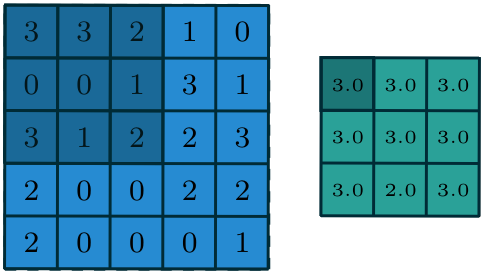
\includegraphics[width=.9\linewidth]{images/max-pooling}
		\caption{Gộp cực đại}
		\label{fig:max-pooling}
	\end{subfigure}

	\begin{subfigure}{.4\textwidth}
		\centering
		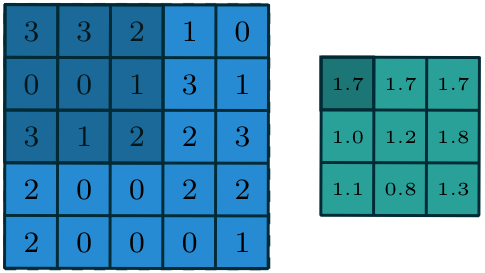
\includegraphics[width=.9\linewidth]{images/avg-pooling}
		\caption{Gộp trung bình}
		\label{fig:avg-pooling}
	\end{subfigure} %
	\caption{Thuật toán gộp cực đại và gộp trung bình với bước nhảy đơn vị}
\end{figure}

Giống như lớp tích chập, lớp gộp cũng có thể sử dụng độ bước nhảy để xác định khoảng cách di chuyển của khung gộp trên ma trận vào. Nếu bước nhảy là 1 hay bước nhảy đơn vị, khung gộp sẽ di chuyển một bước một vị trí trong mỗi lần tính toán. Nếu bước nhảy lớn hơn 1, khung gộp sẽ di chuyển nhanh hơn và kích thước của ma trận kết quả sẽ nhỏ hơn so với đầu vào.

Lớp gộp thường được sử dụng sau mỗi lớp tích chập trong mạng CNN để giảm kích thước không gian của đặc trưng và tổng quát hóa thông tin. Việc giảm kích thước không gian giúp giảm số lượng tham số và tính toán, đồng thời tạo ra các đặc trưng cấp cao hơn bằng cách tóm tắt thông tin từ các vùng lớn hơn của đầu vào.

Tuy nhiên, lớp gộp cũng có một nhược điểm là khiến mất mất một số thông tin chi tiết, vì chỉ giữ lại thông tin quan trọng nhất. Điều này có thể làm mất một số thông tin nhỏ nhưng quan trọng, đặc biệt đối với các bài toán yêu cầu độ chính xác cao.

\subsection{Lớp kích hoạt}
Lớp kích hoạt trong mạng CNN là một lớp không có trọng số và thường được đặt sau mỗi lớp tích chập hoặc lớp kết nối đầy đủ trong mạng.

Nguyên lý hoạt động của lớp kích hoạt như sau:

\begin{itemize}
    \item Đầu vào: Lớp kích hoạt nhận đầu vào từ lớp trước đó trong mạng nơ-ron. Đầu vào có thể là một tensor hoặc một ma trận, tùy thuộc vào kiến trúc của mạng nơ-ron.
    \item Hàm kích hoạt: Lớp kích hoạt áp dụng một hàm kích hoạt phi tuyến tính lên đầu vào. Hàm kích hoạt này thường được chọn để giới hạn đầu ra và tạo độ không tuyến tính cho mạng nơ-ron. Một số hàm kích hoạt phổ biến bao gồm:
    \begin{itemize}
        \item Hàm ReLU (Rectified Linear Unit): $f(x) = max(0, x)$. Nó giữ nguyên giá trị không âm và bỏ qua các giá trị âm.
        \item Hàm Sigmoid: $f(x) = \frac{1}{(1 + exp(-x))}$. Nó chuyển đổi giá trị đầu vào thành một phạm vi từ $0$ đến $1$, thường được sử dụng trong các bài toán phân loại nhị phân.
        \item Hàm Tanh: $f(x) = \frac{(exp(x) - exp(-x))}{(exp(x) + exp(-x))}$. Tương tự như hàm sigmoid, nhưng đầu ra nằm trong khoảng từ $-1$ đến $1$.
        \item Hàm Softmax: $f(x_i) = \frac{exp(x_i)}{sum(exp(x_j))}$, với $i$ là chỉ số của đầu ra và $j$ là chỉ số của tất cả các đầu ra. Hàm softmax thường được sử dụng trong bài toán phân loại đa lớp để chuyển đổi đầu vào thành các xác suất phân loại.
    
    \end{itemize}
    \item Đầu ra: Kết quả của lớp kích hoạt là đầu ra của lớp này, được truyền tới lớp tiếp theo của mạng.
\end{itemize}
    
Lớp kích hoạt chủ yếu được sử dụng để tạo độ không tuyến tính trong mạng nơ-ron và giúp mô hình học được các đặc trưng phức tạp và biểu diễn các mô hình quan hệ phi tuyến. Nó cũng giúp giới hạn đầu ra trong một phạm vi nhất định và tạo ra các đầu ra dễ hiểu và dễ xử lý cho các lớp tiếp theo.

Các hàm kích hoạt và vị trí của lớp kích hoạt trong mạng nơ-ron có thể được điều chỉnh tùy thuộc vào bài toán cụ thể và kiến trúc mạng nơ-ron.

\subsection{Lớp kết nối đầy đủ}
Lớp kết nối đầy đủ còn được gọi là lớp đầu ra trong mạng nơ-ron, là một trong những loại lớp quan trọng trong kiến trúc mạng nơ-ron truyền thẳng.

Nguyên tắc hoạt động của lớp kết nối đầy đủ như sau:

\begin{itemize}
    \item Đầu vào: Lớp kết nối đầy đủ nhận đầu vào từ lớp trước đó trong mạng nơ-ron. Đầu vào thường là một vector hoặc một tensor được duỗi thành một vector.
    \item Trọng số và độ lệch: Mỗi nút trong lớp kết nối đầy đủ kết nối với tất cả các nút trong lớp trước đó thông qua một trọng số (weight) tương ứng. Mỗi kết nối có một trọng số riêng. Ngoài ra, mỗi nút cũng có một độ lệch (bias) tương ứng.
    \item Tính toán: Đầu vào của mỗi nút trong lớp kết nối đầy đủ được nhân với trọng số tương ứng và cộng với độ lệch. Sau đó, kết quả được đưa qua một hàm kích hoạt phi tuyến tính (như hàm ReLU, sigmoid, tanh) để tạo ra đầu ra của nút đó.
    \item Đầu ra: Kết quả tính toán của mỗi nút trong lớp kết nối đầy đủ là đầu ra của lớp này. Đầu ra có thể là một vector hoặc một tensor tùy thuộc vào số lượng nút trong lớp.
\end{itemize}

Lớp kết nối đầy đủ thường được sử dụng trong các mạng nơ-ron truyền thẳng để tạo ra đầu ra cuối cùng của mạng. Nó giúp mô hình học được các mối quan hệ phức tạp giữa đầu vào và đầu ra. Các lớp kết nối đầy đủ thường được sử dụng trong các bài toán như phân loại ảnh, nhận dạng giọng nói, bài toán dự báo, và nhiều bài toán khác.

Một số kiến trúc mạng nơ-ron sử dụng nhiều lớp kết nối đầy đủ liên tiếp nhau để tạo thành một mạng nơ-ron sâu (deep neural network). Trong các mạng nơ-ron sâu, thông qua việc kết hợp nhiều lớp kết nối đầy đủ với các hàm kích hoạt phi tuyến tính, mô hình có khả năng học được các đặc trưng phức tạp và biểu diễn các mô hình quan hệ phi tuyến giữa đầu vào và đầu ra.


\subsection{Mạng tích chập toàn phần}

Mạng tích chập toàn phần (FCN) được sử dụng rộng rãi trong bài toán xử lý ảnh và phân vùng ảnh. So với CNN truyền thống, FCN không có các lớp kết nối đầy đủ ở cuối mạng mà thay vào đó, FCN chỉ sử dụng các lớp tích chập, lớp gộp và kích hoạt trong mạng (Hình \ref{fig:fcn1}). Trong bài toán phân vùng ảnh, mô hình cần gán nhãn cho từng điểm ảnh trong mỗi vùng (Hình \ref{fig:fcn2}). Từ các vùng ảnh, có thể đánh giá hộp bao cho vật thể trong bài toán phát hiện vật thể.

% TODO: \usepackage{graphicx} required
\begin{figure}[h]
	\centering
	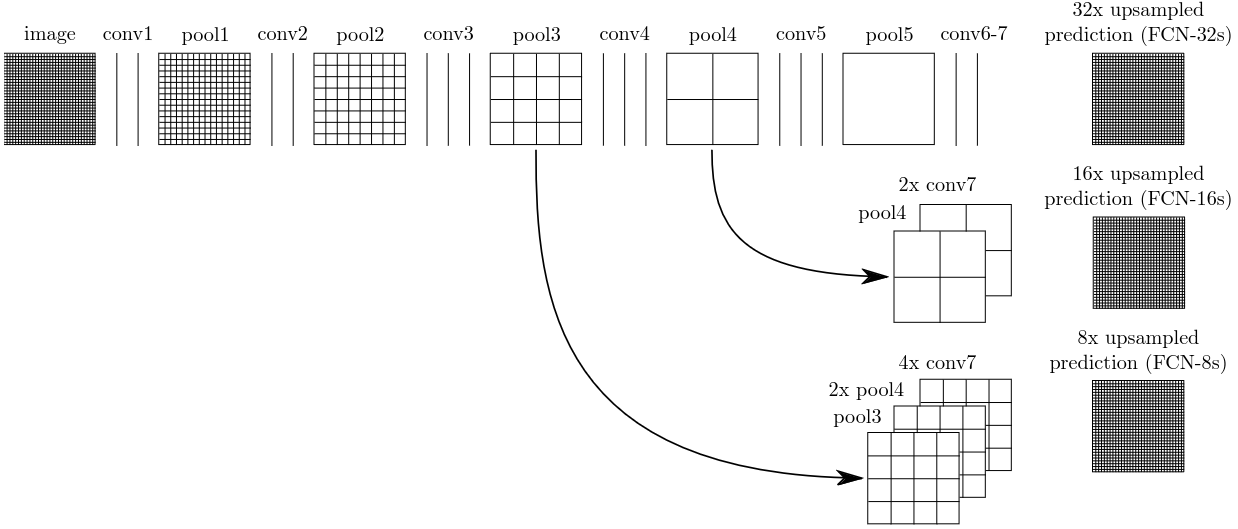
\includegraphics[width=0.99\linewidth]{images/fcn1}
	\caption{Mạng tích chập toàn phần}
	\label{fig:fcn1}
\end{figure}

% TODO: \usepackage{graphicx} required
\begin{figure}[h]
	\centering
	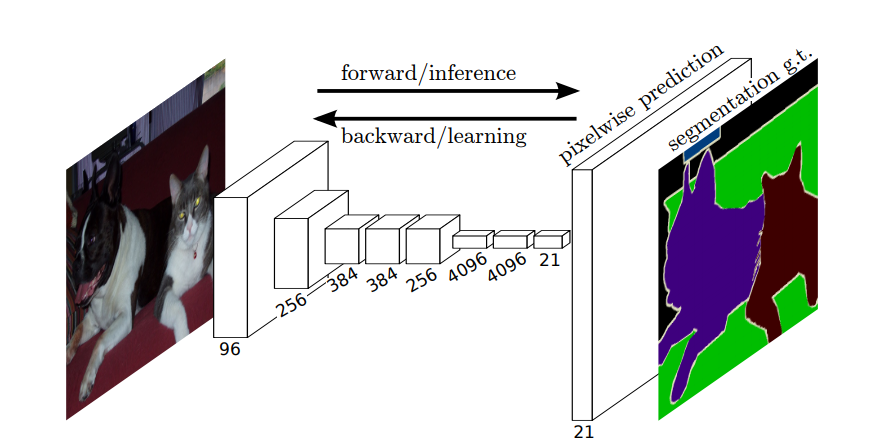
\includegraphics[width=0.9\linewidth]{images/fcn2}
	\caption{Bài toán phân vùng ảnh}
	\label{fig:fcn2}
\end{figure}


\subsection{Mạng đặc trưng kim tự tháp}

Việc phát hiện vật thể trở nên rất thách thức đối với các vật thể nhỏ. Một phương pháp dễ hiểu là sinh đặc trưng với từng tỉ lệ khác nhau như kim tự tháp trên mạng. Tuy nhiên, phương pháp này gây lãng phí tài nguyên tính toán và bộ nhớ. Vì vậy, mạng đặc trưng kim tự tháp (FPN) ra đời với mục tiêu cân bằng giữa độ chính xác và tốc độ xử lý.

FPN bao gồm một đường từ dưới lên và một luồng từ trên xuống. Đường từ dưới lên thực hiện trích xuất đặc trưng. Càng lên cao độ phân giải càng giảm và giá trị thông tin về ngữ cảnh càng cao. Luồng từ trên xuống có chức năng xây dựng các lớp có độ phân giải cao từ các lớp có thông tin ngữ cảnh cao (Hình \ref{fig:fpn}).

% TODO: \usepackage{graphicx} required
\begin{figure}[h]
	\centering
	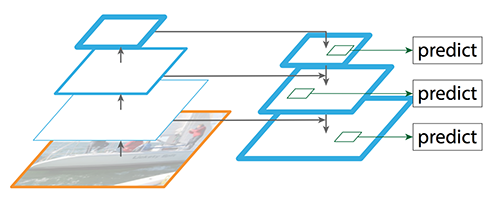
\includegraphics[width=0.8\linewidth]{images/fpn}
	\caption{Mô hình đặc trưng kim tự tháp}
	\label{fig:fpn}
\end{figure}

Trong quá trình xây dựng từ trên xuống, thông tin của đối tượng sẽ bị mất mát. Vì vậy, các kết nối tắt đồng cấp sẽ giúp quá trình dự đoán vị trí các đối tượng tốt hơn, hạn chế tối đa việc mất mát thông tin

\subsection{Hàm mất mát}

Hàm mất mát là một hàm số được sử dụng trong quá trình huấn luyện mô hình máy học để đo lường sự khác biệt giữa các dự đoán của mô hình và giá trị thực tế của dữ liệu đích. Mục tiêu của việc tối ưu hàm mất mát là điều chỉnh các tham số của mô hình để giảm thiểu sai số giữa dự đoán và giá trị thực tế.

Hàm mất mát thường được xây dựng dựa trên mục tiêu cụ thể của vấn đề máy học mà bạn đang giải quyết.

Trong bài toán phát hiện đối tượng, hai hàm mất mát quan trọng nhất là hàm mất mát về lớp đối tượng và hàm mất mát về hộp bao.

Gọi vùng hình ảnh chiếm chỗ thực tế của đối tượng là $A$, vùng hình ảnh dự đoán được của mô hình là $A'$, có thể dễ dàng tính toán được vùng giao và hợp của hai vùng $A$ và $A'$. Hàm mất mát về hộp bao có thể được tính toán từ hai vùng này (Công thức \ref{eqn:iou}).

\begin{equation} 
	\label{eqn:iou}
	IoU=\frac{A\cup A'}{A\cap A'}
\end{equation}

Mọi thay đổi liên quan đến vị trí hoặc hình dạng hộp bao đều làm giảm $IoU$, vì vậy, $IoU$ có thể được sử dụng đánh giá độ chính xác về cả vị trí và hình dạng hộp bao, tối ưu các tham số nhằm sinh $IoU$ cao hơn giúp tăng độ chính xác của mô hình khi xác định hộp bao của vật thể.

Đối với hàm mất mát về lớp đối tượng, hàm mất mát có thể thuộc dạng $1 - 0$, nghĩa là đúng hoặc sai trong dự đoán, hoặc sử dụng phương pháp đo lường sự khác biệt giữa phân phối xác suất dự đoán của mô hình với phân phối xác suất thực tế của các lớp.

Gọi $y_i$ là xác suất của lớp thứ $i$ trong tập dữ liệu, $y'_i$ là xác suất của lớp $i$ trong tập dự đoán, có thể xây dựng hàm mất mát như công thức \ref{eqn:ce-loss}. Như vậy, nếu xác suất dự đoán chính xác càng thấp, giá trị mất mát càng nhỏ và ngược lại.

\begin{equation}
	\label{eqn:ce-loss}
	L_{CE} = - \sum_{i = 1}^{n}y_ilog(y'_i)
\end{equation}


\subsection{Học có giám sát}




\subsection{Đánh giá hiệu suất của mạng nơ-ron tích chập}
Trong mạng nơ-ron tích chập (CNN), có một số thông số quan trọng được sử dụng để đánh giá hiệu suất của mô hình:
\begin{itemize}
	\item  Độ chính xác $Accuracy$ là tỷ lệ phần trăm của số lượng dự đoán chính xác trên tổng số lượng dự đoán. Độ chính xác được tính bằng công thức \ref{eqn-acc}.
	\begin{equation}
		\label{eqn:acc}
		Accuracy = \frac{TP + TN}{TP + TN + FP + FN}
	\end{equation}
	
	\item Độ chính xác dương tính $Precision$ đo lường tỷ lệ giữa số lượng dự đoán dương tính chính xác và tổng số lượng dự đoán dương tính. Đây là tỉ lệ giữa số lượng dự đoán "đúng" chính xác và tổng số lượng dự đoán "đúng" (Công thức \ref{eqn:prec}).
	\begin{equation}
		\label{eqn:prec}
		Precision = \frac{TP}{TP + FP}
	\end{equation}	
	\item Độ nhớ tìm kiếm $Recall$ còn được gọi là độ nhạy, đo lường tỷ lệ giữa số lượng dự đoán dương tính chính xác và tổng số lượng thực tế dương tính. Đây là tỉ lệ giữa số lượng dự đoán "đúng" chính xác và tổng số lượng dự đoán "đúng" thực tế.
	\begin{equation}
		\label{eqn:recall}
		Recall = \frac{TP}{TP + FN}
	\end{equation}	
	
	\item Điểm F1 là một đánh giá tổng hợp, kết hợp giữa Độ chính xác dương tính và độ nhạy. Nó đo lường sự cân bằng giữa độ chính xác dương tính và độ nhạy. 
	\begin{equation}
		\label{eqn:f1}
		F1_{score} = \frac{2 * (Precision * Recall)}{(Precision + Recall)}
	\end{equation}
	
\end{itemize}


\section{Mô hình YOLO}

\subsection{Giới thiệu mô hình}

Mô hình YOLO là một mô hình phổ biến trong lĩnh vực nhận diện đối tượng và phát hiện vị trí đối tượng trong ảnh và video. Mô hình YOLO có khả năng phân loại và định vị các đối tượng trong một khung hình duy nhất một cách nhanh chóng và chính xác.

Các đặc điểm chính của mô hình YOLO bao gồm:
\begin{itemize}
    \item Kiến trúc: Mô hình YOLO sử dụng mạng nơ-ron tích chập (CNN) để trích xuất đặc trưng từ ảnh đầu vào và dự đoán các hộp giới hạn\ và các lớp đối tượng tương ứng. Kiến trúc gốc của YOLO được gọi là YOLOv1 và sau đó đã có các phiên bản cải tiến như YOLOv2, YOLOv3,  YOLOv4, YOLOv5, YOLOv8, ...
    \item Grid cells: Mô hình YOLO chia ảnh thành một lưới ô vuông có kích thước cố định. Mỗi ô vuông trong lưới được gọi là một grid cell. Mỗi grid cell sẽ dự đoán một số lượng hộp giới hạn và lớp đối tượng tương ứng.
    \item Dự đoán hộp giới hạn: Mỗi grid cell trong mô hình YOLO dự đoán các hộp giới hạn bằng cách dùng các tỷ lệ (scales). Mỗi hộp giới hạn được biểu diễn bằng các thông số như tọa độ (x, y) của trung tâm, chiều rộng và chiều cao của hộp.
    \item Dự đoán lớp đối tượng: Mô hình YOLO dự đoán lớp đối tượng của mỗi hộp giới hạn bằng cách sử dụng softmax trên các điểm đặc trưng (feature points) của ảnh.
    \item Non-max suppression: Sau khi mô hình YOLO đã dự đoán các hộp giới hạn và lớp đối tượng, một quá trình gọi là non-max suppression được áp dụng để loại bỏ các hộp giới hạn trùng lặp và giữ lại các hộp giới hạn có xác suất dự đoán cao nhất.
\end{itemize}


\subsection{Kiến trúc mạng của mô hình}

Kiến trúc mạng YOLO (You Only Look Once) đã trải qua nhiều phiên bản và cải tiến, bao gồm YOLOv1, YOLOv2, YOLOv3 đến YOLOv8. Tuy nhiên, YOLO hiện nay bao gồm các thành phần chính như: Backbone, Neck và Head.

\begin{itemize}
    \item Backbone network: YOLO sử dụng một mạng nơ-ron tích chập (CNN) làm cơ sở để trích xuất đặc trưng từ ảnh. Mạng nền (backbone network) trong YOLO có thể được xây dựng bằng cách sử dụng các kiến trúc như Darknet hoặc CSPDarknet.
    \item Neck: YOLO có một phần gọi là neck (cổ), được đặt giữa backbone network và head của mô hình. Neck có nhiệm vụ kết hợp các đặc trưng từ các tầng khác nhau của feature pyramid để cung cấp thông tin phong phú hơn cho việc dự đoán đối tượng.
    \item Head: Đây là phần cuối cùng của mô hình YOLO, nơi các hộp giới hạn và lớp đối tượng được dự đoán. Head của YOLO sử dụng các lớp tích chập để dự đoán tọa độ và lớp của các hộp giới hạn. Đồng thời, YOLO sử dụng các kỹ thuật như SPP (Spatial Pyramid Pooling) và PANet (Path Aggregation Network) để cải thiện khả năng phát hiện và định vị đối tượng.
\end{itemize}

Với hàm mất mát, mô hình YOLO sử dụng một hàm mất mát kết hợp giữa các thành phần như localization loss, confidence loss và class loss. Hàm mất mát này giúp tối ưu hóa mô hình và cải thiện độ chính xác của các dự đoán.

\subsection{Đánh giá hiệu suất của mô hình}

Qua các phiên bản, mô hình YOLO ngày càng được cải thiện. Hình \ref{fig:yolov8-better} cho thấy các phiên bản YOLO ngày càng được cải thiện với lượng tham số nhỏ hơn nhanh hơn nhưng hiệu suất lại cao hơn.

\begin{figure}
    \centering
    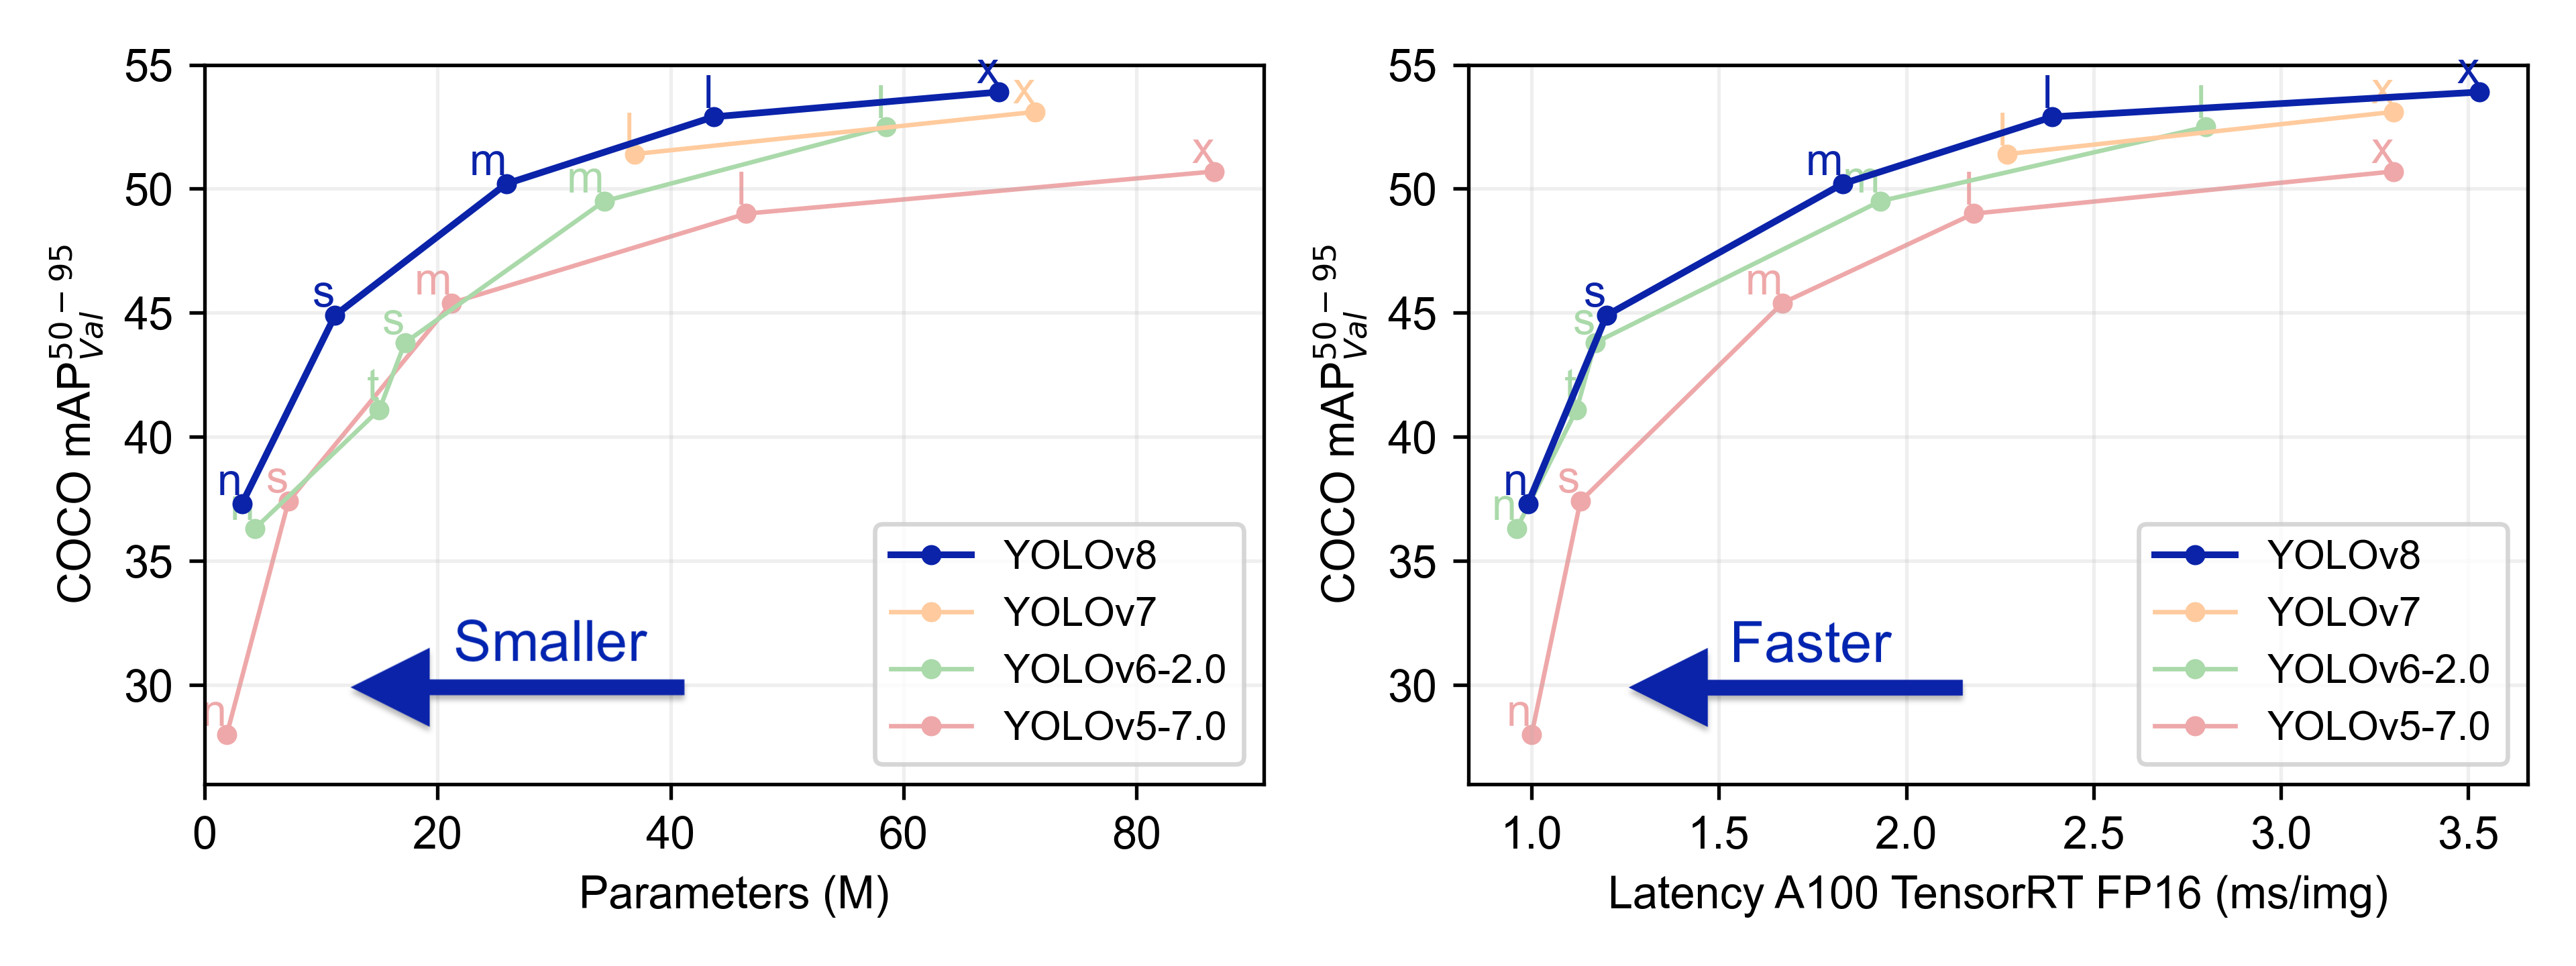
\includegraphics[width=0.75\linewidth]{images/yolov8-better.png}
    \caption{yolov8-better}
    \label{fig:yolov8-better}
\end{figure}
\subsection{So sánh YOLO và CNN trong nhận diện và phân loại ảnh}


\subsubsection{Kiến trúc mạng}
CNN là một kiến trúc mạng nơ-ron sử dụng các tầng tích chập và tầng kết nối đầy đủ để học các đặc trưng của ảnh. CNN thường sử dụng một số tầng tích chập để trích xuất đặc trưng và sau đó sử dụng các tầng kết nối đầy đủ để phân loại ảnh.

YOLO là một kiến trúc mạng nơ-ron đặc biệt được thiết kế cho việc phát hiện và định vị đối tượng trong ảnh. YOLO chia ảnh thành các lưới (grid) và dự đoán các hộp giới hạn (bounding box) và lớp đối tượng cho mỗi lưới. YOLO sử dụng một kiến trúc mạng nơ-ron tích chập để trích xuất đặc trưng và dự đoán đồng thời các hộp giới hạn và lớp đối tượng.

\subsubsection{Tốc độ}

Với CNN, việc phân loại và nhận dạng đối tượng được thực hiện trong các lớp cuối cùng của mạng. Điều này có nghĩa là CNN phải đi qua toàn bộ hình ảnh để đưa ra dự đoán, do đó, tốc độ của CNN thường chậm hơn so với YOLO.

YOLO sử dụng một phương pháp "You Only Look Once" để dự đoán đồng thời các hộp giới hạn và lớp đối tượng trên toàn bộ ảnh. Điều này giúp YOLO có tốc độ rất nhanh, vì nó không cần phải xem xét ảnh nhiều lần.

\subsubsection{Độ chính xác}

Với việc sử dụng các tầng tích chập và kết nối đầy đủ, CNN có thể học các đặc trưng phức tạp từ ảnh và đạt được độ chính xác cao trong các tác vụ phân loại và nhận dạng ảnh.

YOLO có thể cung cấp độ chính xác tương đối cao trong việc phát hiện và định vị đối tượng trong ảnh. Tuy nhiên, do việc dự đoán đồng thời trên toàn bộ ảnh, YOLO có xu hướng không chính xác hơn trong việc định vị các đối tượng nhỏ hoặc gần nhau.

\section{Nghiên cứu ứng dụng CNN và YOLO trong hệ thống theo dõi và chăm sóc nấm}

Với độ chính xác tương đối cao với tác vụ phân loại vật thể và khả năng xác định vùng bao vật thể, mô hình YOLO có thể ứng dụng trong hệ thống theo dõi và chăm sóc nấm. Bằng việc xây dựng bộ dữ liệu với các loại nấm cùng giai đoạn phát triển khác nhau, mô hình có thể cho ra biết vị trí, thời gian và giai đoạn phát triển hiện tại, giúp người nông dân đưa ra quyết định kịp thời hoặc có thể hỗ trợ điều khiển robot tự động làm việc chăm sóc hay chuẩn bị,  thu hoạch nấm.

\section{Hướng phát triển và nâng cao hiệu suất mô hình CNN và YOLO}

Đối với mô hình YOLOv8, mô hình có thể được điều chỉnh với các kích thước khác nhau (Hình \ref{fig:yolov8-structure}).

\begin{figure}
    \centering
    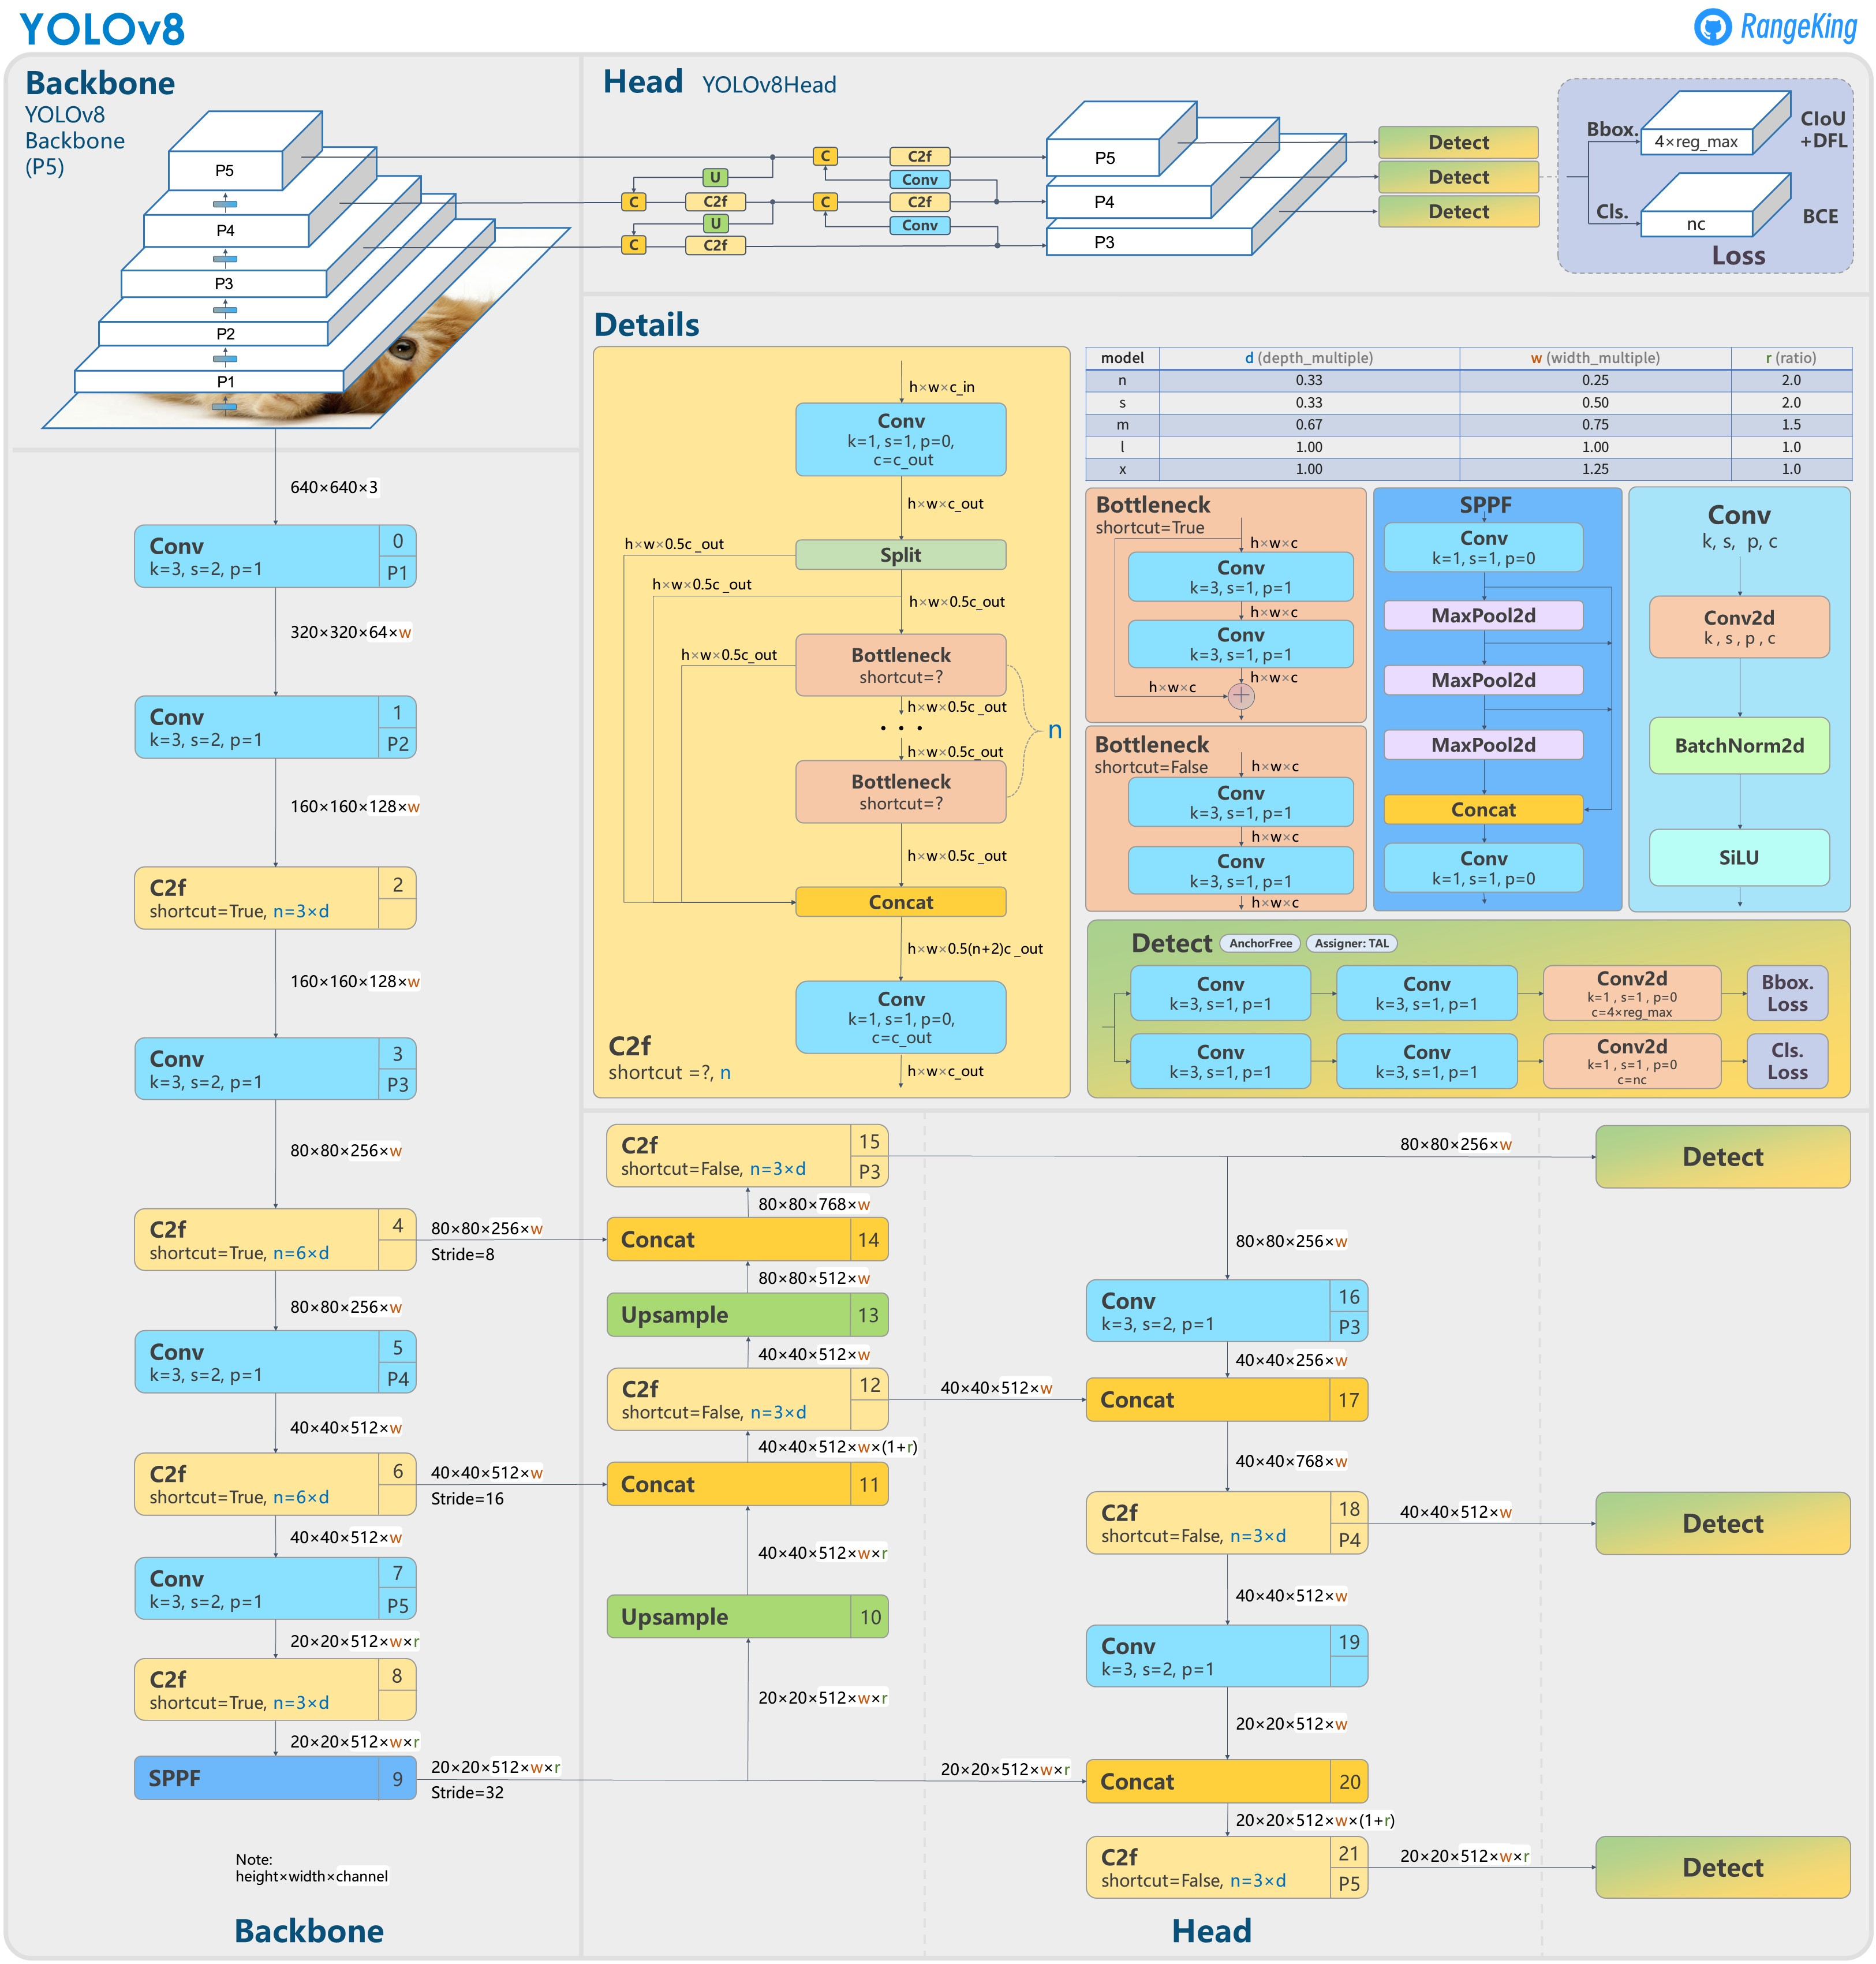
\includegraphics[width=1\linewidth]{images/yolov8-network.png}
    \caption{Cấu trúc mạng YOLOv8 và cấu hình kích thước}
    \label{fig:yolov8-structure}
\end{figure}

Với kích thước lớn - L, mô hình có khả năng học sâu hơn và đưa ra kết quả chính xác hơn. Tuy nhiên, dữ liệu đầu vào cần đa dạng và số lượng lớn hơn để có thể lấy ra những đặc trưng một cách chung nhất. Đối với số lượng mẫu nhỏ, để tránh tình trạng overfitting, kích thước nhỏ như s, n sẽ phù hợp hơn.

\section{Tổng kết chương}


Chương 2 tập trung nghiên cứu ứng dụng của mạng nơ-ron tích chập và mô hình YOLO trong hệ thống theo dõi và chăm sóc nấm.

Trước tiên, mạng nơ-ron tích chập là một mô hình học sâu được thiết kế đặc biệt cho việc xử lý dữ liệu hình ảnh. Nguyên lý hoạt động mạng dựa trên phép tích chập để lấy ra đặc trưng của ảnh, từ đó có thể phân loại ảnh vào các lớp khác nhau.

Tiếp theo, YOLO là một mô hình phát hiện và định vị đối tượng trong ảnh. Với việc chia ảnh thành các ô lưới và dự đoán hộp giới hạn và xác suất cho các đối tượng trong mỗi ô lưới, YOLO mang lại khả năng phát hiện đối tượng nhanh chóng và chính xác.

Cuối cùng là khả năng áp dụng YOLO vào hệ thống giám sát và chăm sóc nấm. Bằng việc phát hiện giai đoạn phát triển và vị trí của nấm, các công việc phân tích, chăm sóc có thể được thực hiện kịp thời. Ngoài ra, chương 2 còn để cập đến hướng phát triển và nâng cao hiệu suất của mô hình CNN và YOLO.

Như vậy, có thể thấy rằng CNN và YOLO có thể được ứng dụng trong hệ thống theo dõi và chăm sóc nấm. Sử dụng các phương pháp này, quá trình phân loại, phát hiện và định vị nấm có thể được tự động hóa, giúp tăng hiệu suất và chính xác, đồng thời giảm công sức và chi phí nhân công.

% !TeX root = ../main.tex
\chapter{XÂY DỰNG HỆ THỐNG}
\section{Phân tích yêu cầu}

\subsection{Sơ đồ usecase chính}


\begin{figure}[h]
	\centering
	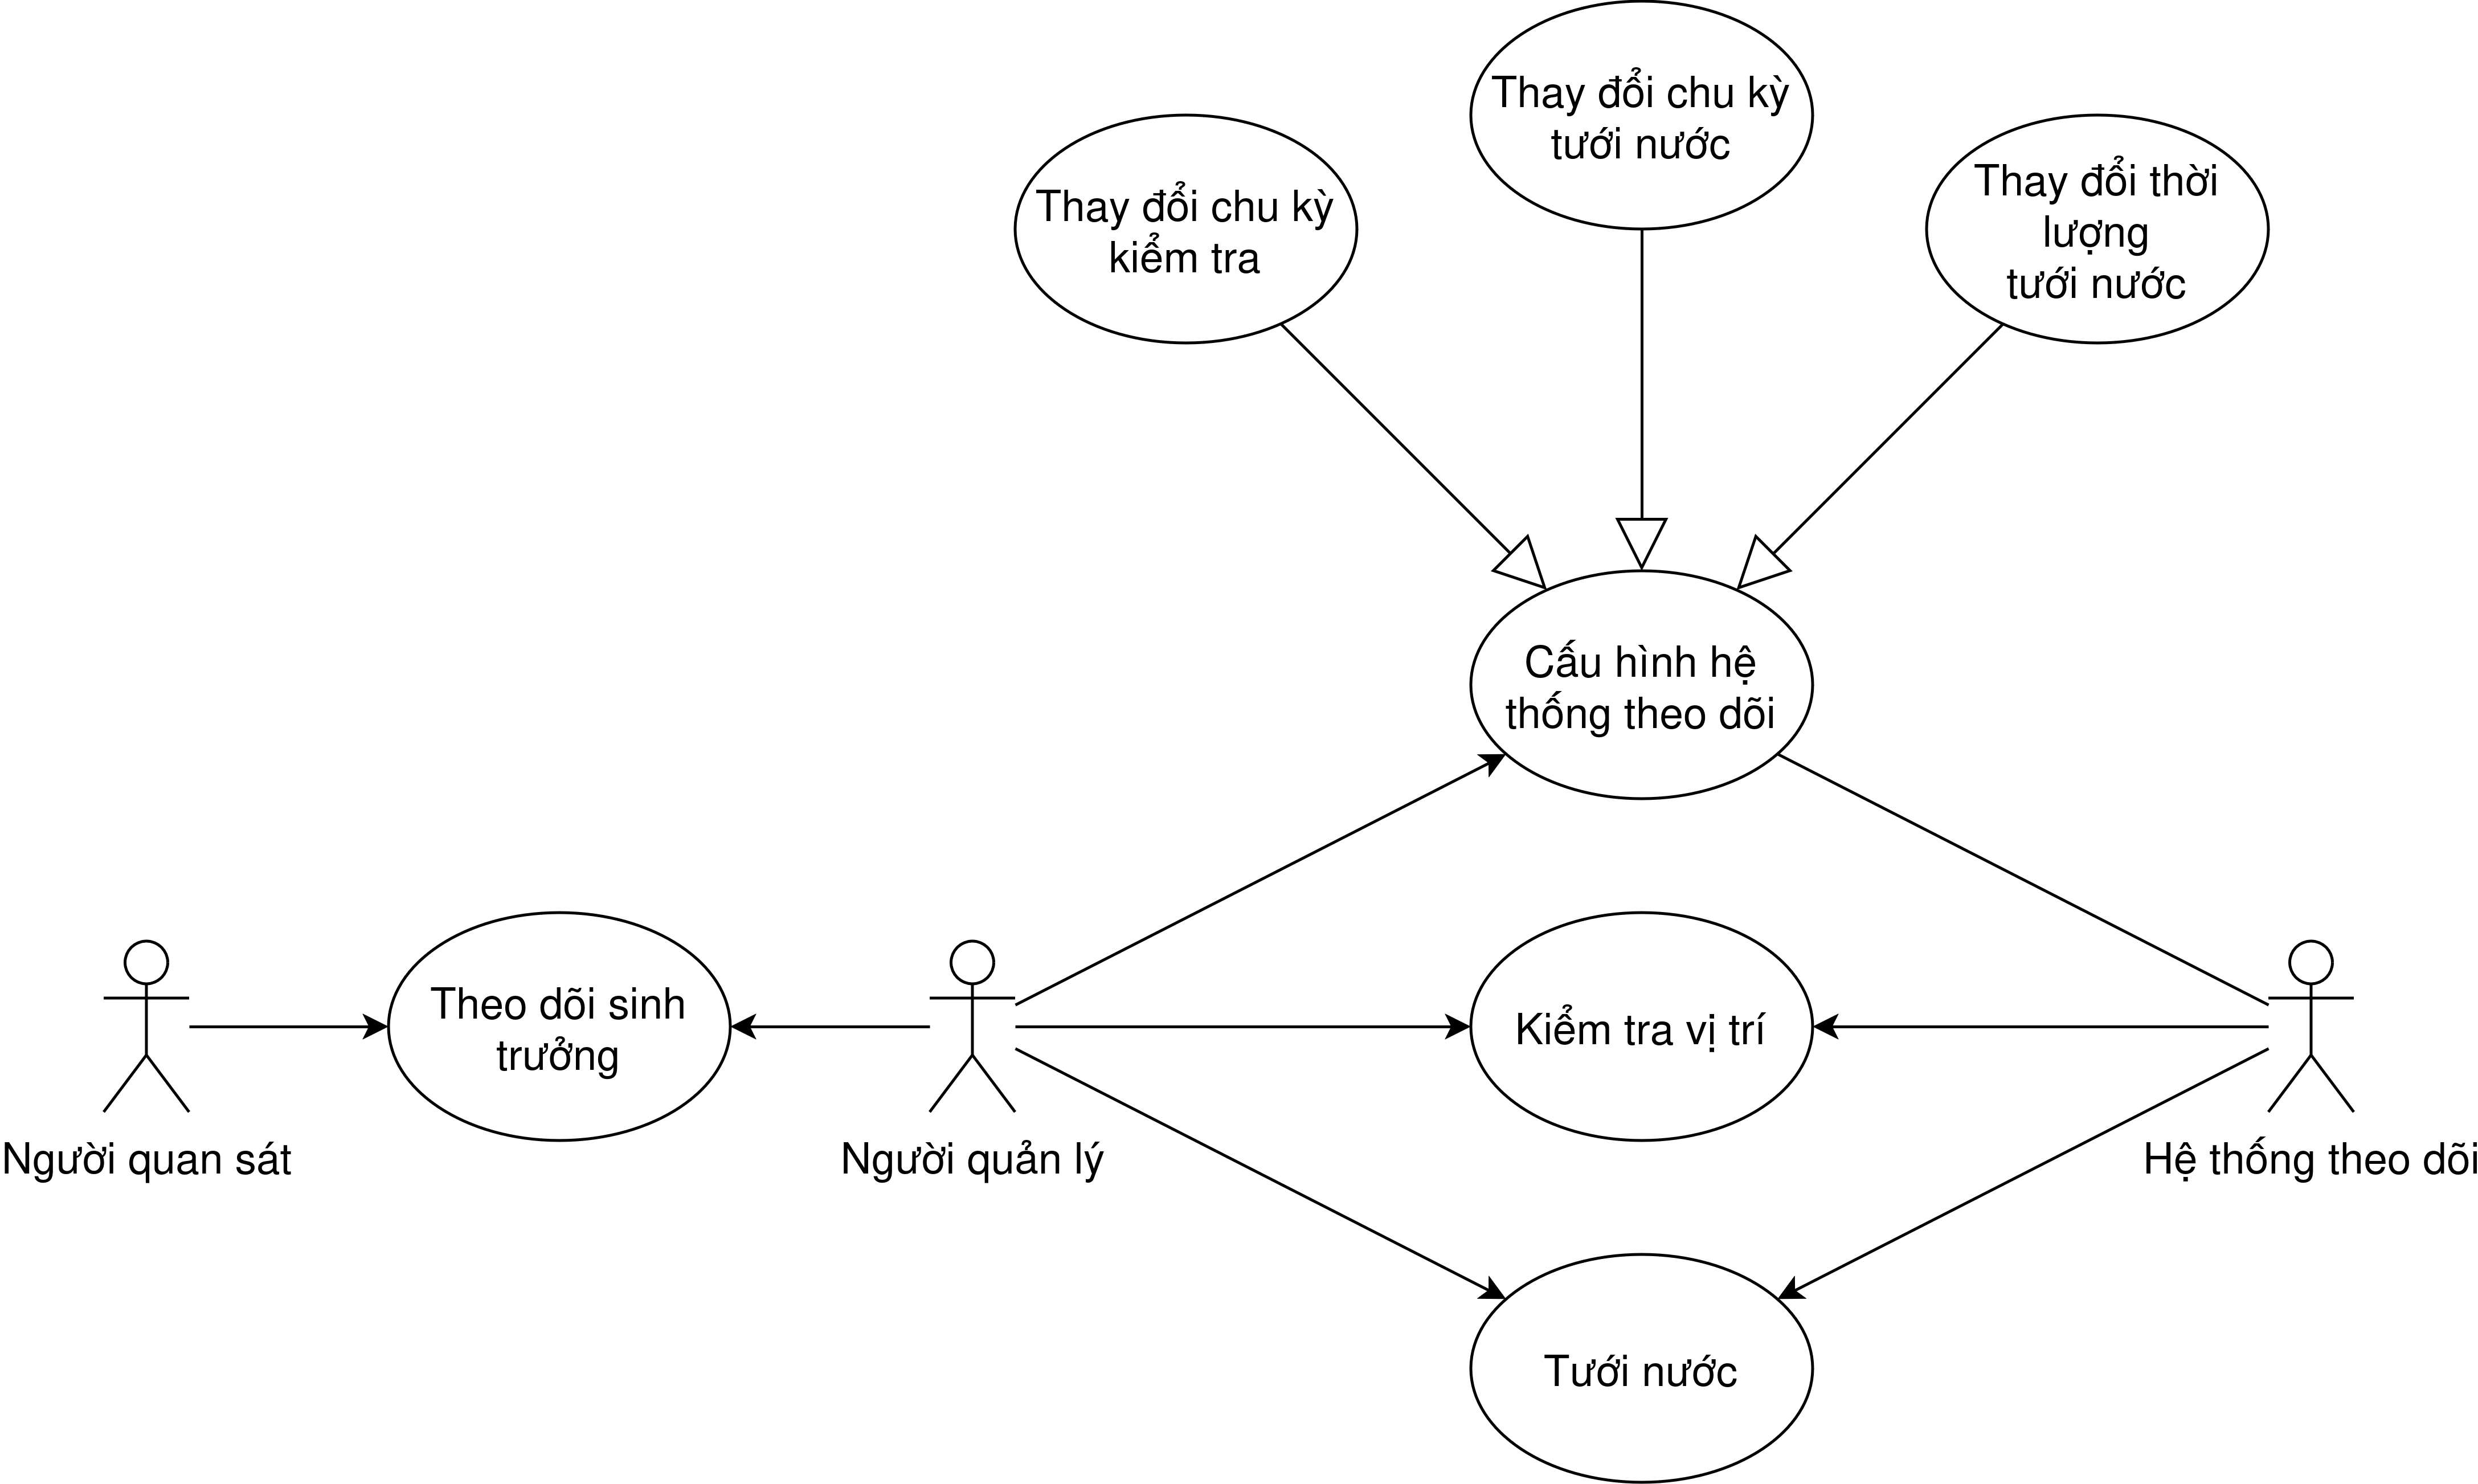
\includegraphics[width=\linewidth]{images/main-usecase}
	\caption{Usecase chính}
	\label{fig:main-usecase}
\end{figure}

\subsubsection{Đặc tả usecase tưới nước}

% Please add the following required packages to your document preamble:
% \usepackage{longtable}
% Note: It may be necessary to compile the document several times to get a multi-page table to line up properly
\begin{longtable}[c]{|l|p{11cm}|}
	\caption{Đặc tả usecase tưới nước}
	\label{tab:des-water}\\
	\hline
	\textbf{Usecase} & \textbf{Nội dung}                                                                                  \\ \hline
	\endfirsthead
	\hline
	\textbf{Usecase} & \textbf{Nội dung}                                                                                  \\ \hline
	\endhead
	%
	Tên usecase      & Tưới nước                                                                                          \\ \hline
	Mô tả               & Cho phép người quản lý hoặc hệ thống tưới nước tại vị trí chỉ định.                                \\ \hline
	Người dùng          & Người quản lý, hệ thống theo dõi tự động.                                                          \\ \hline
	Điều kiện kích hoạt & Khi người quản lý muốn thực hiện tưới nước thủ công hoặc tự động tưới sau một khoảng thời gian đặt sẵn. \\ \hline
	Tiền điều kiện      & Người quản lý đăng nhập thành công vào hệ thống.                                                   \\ \hline
	Hậu điều kiện       & Vị trí phôi nấm được tưới nước và ghi nhận vào hệ thống.                                           \\ \hline
	Luồng sự kiện chính &
	\begin{tabular}[c]{p{10.5cm}}1. Người quản lý truy cập trang “Dashboard”.\\ 2. Người quản lý chọn thẻ tương ứng với phôi nấm muốn tưới.\\ 3. Người quản lý nhấn “Water”.\\ 4. Hệ thống thực hiện di chuyển tới vị trí tưới nấm, kiểm tra và tươi nấm.\\ 5. Hệ thống hiển thị hình ảnh tưới nấm và cập nhật lại trang.\end{tabular} \\ \hline
	Luồng sự kiện thay thế &
	\begin{tabular}[c]{p{10.5cm}}
		\textbf{- Hoạt động tưới bởi hệ thống theo dõi tự động:}\\
		1. Hệ thống theo dõi kiểm tra vị trí nấm theo chu kỳ kiểm tra được cài đặt sẵn.\\
		2. Khi lần tưới trước xảy ra vượt quá chu kỳ tưới nước, thực hiện di chuyển, kiểm tra và tưới nấm theo cài đặt.\\
		\textbf{- Tưới nước theo từng trạng thái phát triển:}\\
		1. Người quản lý truy cập trang "Dashboard"\\
		2. Người quản lý chọn trạng thái phát triển tương ứng trong bảng điều khiển\\
		3. Hệ thống lọc các vị trí phù hợp với trạng thái được chọn và hiển thị lên bảng điều khiển.\\
		4. Người dùng nhấn "Water All"\\
		5. Hệ thống di chuyển tới từng vị trí tương ứng và kiểm tra, tưới nấm
	\end{tabular} \\ \hline
\end{longtable}

\subsubsection{Đặc tả usecase kiểm tra vị trí}

% Please add the following required packages to your document preamble:
% \usepackage{longtable}
% Note: It may be necessary to compile the document several times to get a multi-page table to line up properly
\begin{longtable}[c]{|l|p{11cm}|}
	\caption{Đặc tả usecase kiểm tra vị trí}
	\label{tab:des-check}\\
	\hline
	\textbf{Usecase} & \textbf{Nội dung}                                                                                  \\ \hline
	\endfirsthead
	\hline
	\textbf{Usecase} & \textbf{Nội dung}                                                                                  \\ \hline
	\endhead
	%
	Tên usecase      & Kiểm tra vị trí                                                                                         \\ \hline
	Mô tả               & Cho phép người quản lý hoặc hệ thống kiểm tra trạng thái của vị trí chỉ định.                                \\ \hline
	Người dùng          & Người quản lý, hệ thống theo dõi tự động.                                                          \\ \hline
	Điều kiện kích hoạt & Khi người quản lý muốn thực hiện kiểm tra thủ công hoặc tự động kiểm tra sau một khoảng thời gian đặt sẵn. \\ \hline
	Tiền điều kiện      & Người quản lý đăng nhập thành công vào hệ thống.                                                   \\ \hline
	Hậu điều kiện       & Vị trí phôi nấm được tưới nước và ghi nhận vào hệ thống.                                           \\ \hline
	Luồng sự kiện chính &
	\begin{tabular}[c]{p{10.5cm}}
		1. Người quản lý truy cập trang “Dashboard”.\\
		2. Người quản lý chọn thẻ tương ứng với phôi nấm muốn tưới.\\
		3. Người quản lý nhấn “Check”.\\
		4. Hệ thống thực hiện di chuyển tới vị trí tưới nấm, kiểm tra và tươi nấm nếu tới chu kỳ tưới.\\
		5. Hệ thống hiển thị hình ảnh tưới nấm và cập nhật lại trang.
	\end{tabular} \\ \hline
	Luồng sự kiện thay thế &
	\begin{tabular}[c]{p{10.5cm}}
		\textbf{- Hoạt động tưới bởi hệ thống theo dõi tự động}\\
		1. Hệ thống theo dõi kiểm tra vị trí nấm theo chu kỳ kiểm tra được cài đặt sẵn.\\
		2. Khi lần kiểm tra trước xảy ra vượt quá chu kỳ kiểm tra, thực hiện di chuyển, kiểm tra và tưới nấm nếu đạt điều kiện theo cài đặt.\\
		\textbf{- Kiểm tra theo từng trạng thái phát triển:}\\
		1. Người quản lý truy cập trang "Dashboard"\\
		2. Người quản lý chọn trạng thái phát triển tương ứng trong bảng điều khiển\\
		3. Hệ thống lọc các vị trí phù hợp với trạng thái được chọn và hiển thị lên bảng điều khiển.\\
		4. Người dùng nhấn "Check All"\\
		5. Hệ thống di chuyển tới từng vị trí tương ứng, kiểm tra và tưới nấm nếu thỏa mãn điều kiện tưới tự động.
	\end{tabular} \\ \hline
\end{longtable}

\subsubsection{Đặc tả usecase cấu hình hệ thống theo dõi}
% Please add the following required packages to your document preamble:
% \usepackage{longtable}
% Note: It may be necessary to compile the document several times to get a multi-page table to line up properly
\begin{longtable}[c]{|l|p{11cm}|}
	\caption{Đặc tả usecase ucấu hình hệ thống theo dõi}
	\label{tab:des-stage-config}\\
	\hline
	\textbf{Usecase} & \textbf{Nội dung}                                                                                  \\ \hline
	\endfirsthead
	\hline
	\textbf{Usecase}    & \textbf{Nội dung}                                                                                              \\ \hline
	\endhead
	%
	Tên usecase         & Cấu hình hệ thống theo dõi.                                                                                    \\ \hline
	Mô tả                  & Cho phép người quản lý cấu hình hoạt động của hệ thống theo dõi tự động cho từng giai đoạn phát triển của nấm. \\ \hline
	Người dùng             & Người quản lý.                                                                                                 \\ \hline
	Điều kiện kích hoạt    & Khi người quản lý muốn cấu hình hệ thống theo dõi tự động theo chu kỳ đặt sẵn.                                 \\ \hline
	Tiền điều kiện         & Người quản lý đăng nhập thành công vào hệ thống.                                                               \\ \hline
	Hậu điều kiện          & Hệ thống theo dõi tự động được cấu hình thành công và hoạt động theo cấu hình mới                              \\ \hline
	Luồng sự kiện chính &
	\begin{tabular}[c]{p{10.5cm}}1. Người quản lý truy cập trang “Stage Management”.\\ 2. Người quản lý nhập giá trị “chu kỳ kiểm tra”, “chu kỳ tưới nước” và “thời lượng tưới” cho một giai đoạn phát triển và nhấn “Update”.\\ 3. Hệ thống ghi nhận giá trị cấu hình mới và cập nhật lại trang.\end{tabular} \\ \hline
	Luồng sự kiện thay thế & Không                                                                                                          \\ \hline
\end{longtable}

\subsubsection{Đặc tả usecase theo dõi sinh trưởng}

\begin{longtable}[c]{|l|p{11cm}|}
	\caption{Đặc tả usecase theo dõi sinh trưởng}
	\label{tab:des-monitor}\\
	\hline
	\textbf{Usecase} & \textbf{Nội dung}                                                                                  \\ \hline
	\endfirsthead
	\hline
	\textbf{Usecase}    & \textbf{Nội dung}                                                                                              \\ \hline
	\endhead
	%
	Tên usecase         & Theo dõi sinh trưởng.              \\ \hline
	Mô tả                  & Cho phép người quản lý hoặc người quan sát theo dõi sự phát triển của nấm qua thời gian tại vị trí được chọn. \\ \hline
	Người dùng             & Người quản lý, người quan sát. \\ \hline
	Điều kiện kích hoạt    & Khi người quản lý hoặc người quan sát muốn theo dõi sự phát triển của nấm tại các vị trí xác định.                                 \\ \hline
	Tiền điều kiện         & Người quản lý hoặc người quan sát đăng nhập thành công vào hệ thống.                                                               \\ \hline
	Hậu điều kiện          & Hệ thống hiển thị giao diện quản lý cho các vị trí được chỉ định.                              \\ \hline
	Luồng sự kiện chính &
	\begin{tabular}[c]{p{10.5cm}}
		1. Người quản lý hoặc người quan sát truy cập trang “Dashboard”.\\ 
		2. Hệ thống hiển thị các vị trí nấm và hình ảnh của lần kiểm tra gần nhất của từng vị trí.
	\end{tabular} \\ \hline
	Luồng sự kiện thay thế & 	\begin{tabular}[c]{p{10.5cm}}
		\textbf{- Lọc hiển thị từng trạng thái phát triển}\\
		1. Người quản lý hoặc người quan sát truy cập trang “Dashboard”.\\ 
		2. Hệ thống hiển thị các vị trí nấm và hình ảnh của lần kiểm tra gần nhất của từng vị trí.\\
		3. Người quản lý hoặc người quan sát chọn trạng thái sinh trưởng tương ứng trên bảng điều khiển.\\
		4. Hệ thống lọc các vị trí thỏa mãn và hiển thị trên bảng điều khiển.m\\
		\textbf{- Hiển thị một vị trí xác dịnh}\\
		1. Người quản lý hoặc người quan sát truy cập trang “Dashboard”.\\ 
		2. Hệ thống hiển thị các vị trí nấm và hình ảnh của lần kiểm tra gần nhất của từng vị trí.\\
		3. Người quản lý hoặc người quan sát nhấn vào hình ảnh hoặc vị trí tương ứng trong danh sách vị trí.\\
		4. Hệ thống hiển thị chi tiết thông tin của vị trí cùng lịch sử kiểm tra, tưới nước.
	\end{tabular} \\ \hline
\end{longtable}

\subsection{Sơ đồ usecase cho người quản trị}

\begin{figure}[H]
	\centering
	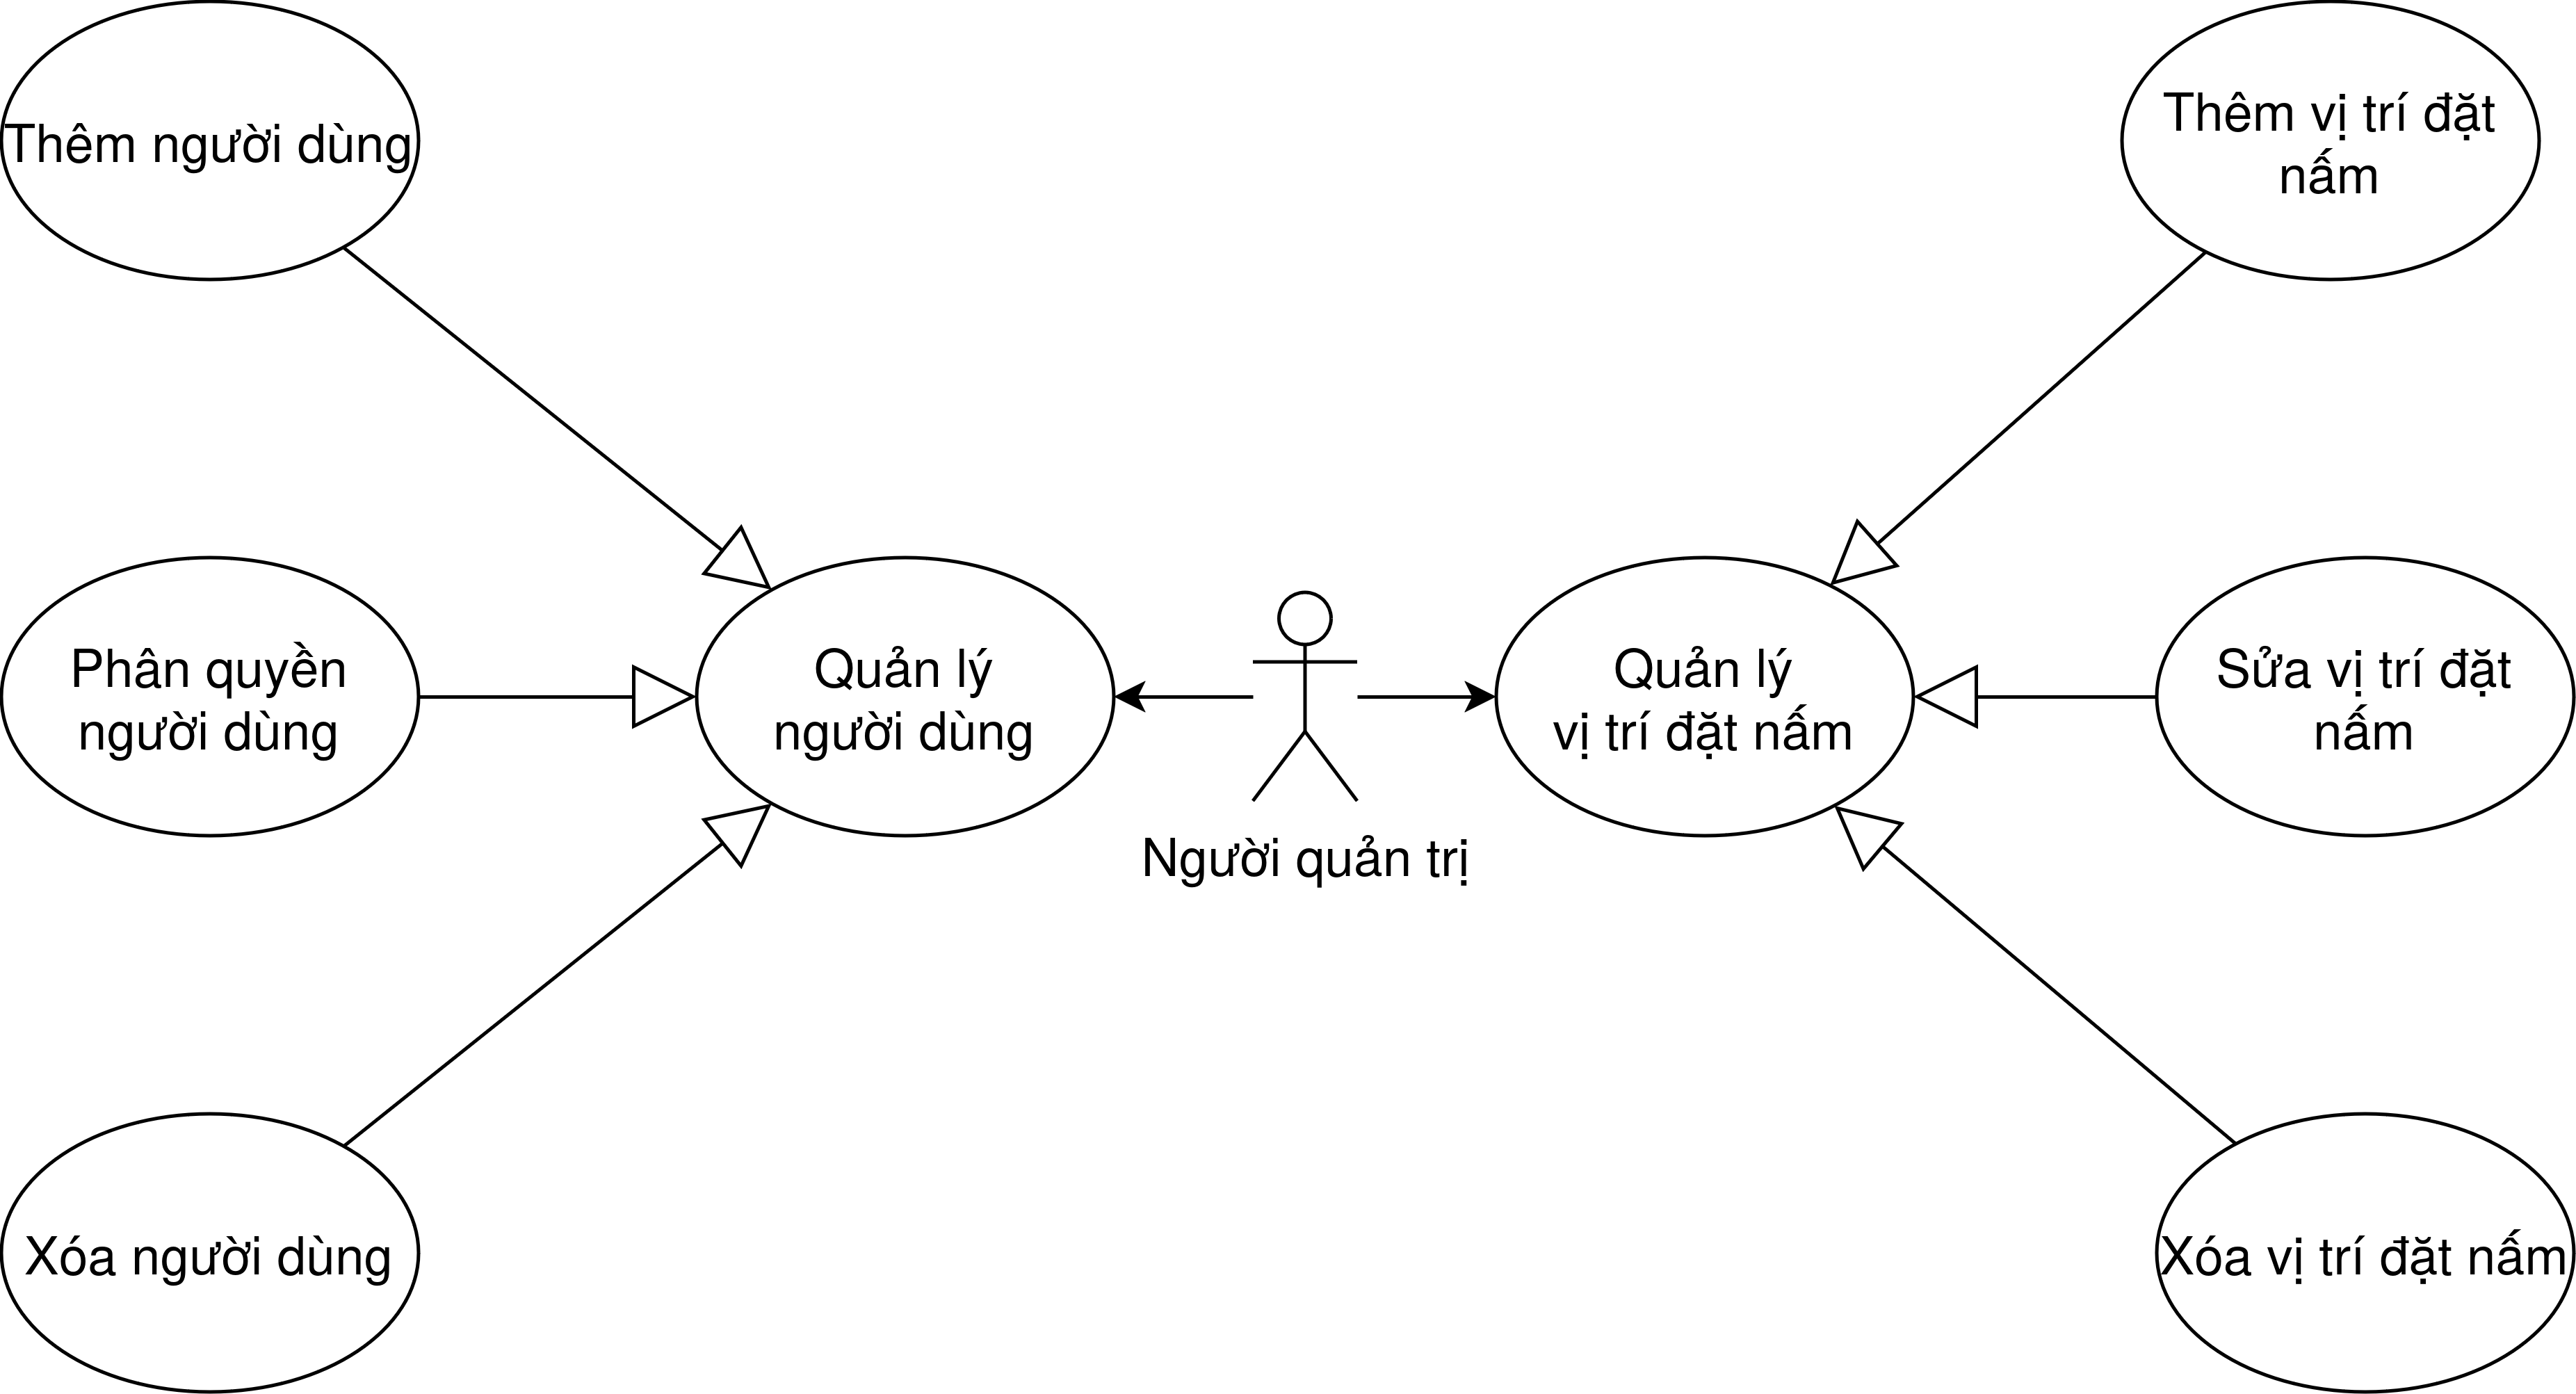
\includegraphics[width=\linewidth]{images/admin-usecase}
	\caption{Usecase cho người quản trị}
	\label{fig:admin-usecase}
\end{figure}
\subsubsection{Đặc tả usecase thêm người dùng}

% Please add the following required packages to your document preamble:
% \usepackage{longtable}
% Note: It may be necessary to compile the document several times to get a multi-page table to line up properly
\begin{longtable}[c]{|l|p{11cm}|}
	\caption{Đặc tả usecase thêm người dùng}
	\label{tab:des-create-user}\\
	\hline
\textbf{Usecase} & \textbf{Nội dung}                                                                                  \\ \hline
\endfirsthead
\hline
\textbf{Usecase}    & \textbf{Nội dung}                                                                                              \\ \hline
\endhead
	%
	Tên usecase      & Thêm người dùng                                                                        \\ \hline
	Mô tả               & Cho phép người quản trị tạo tài khoản người dùng với quyền hạn tương ứng.                                                \\ \hline
	Người dùng          & Người quản trị hệ thống                                                              \\ \hline
	Điều kiện kích hoạt & Người quản trị muốn tạo tài khoản cho người theo dõi hoặc người quản lý chăm sóc nấm hoặc người quản trị khác.\\ \hline
	Tiền điều kiện      & Tên tài khoản không tồn tại                                                          \\ \hline
	Hậu điều kiện       & Tài khoản tạo thành công.                                                             \\ \hline
	Luồng sự kiện chính &
	\begin{tabular}[c]{p{10.5cm}}
		1. Người quản trị nhấn vào mục “User Management”. \\ 
		2. Hệ thống hiển thị trang quản trị người dùng với danh sách người dùng hiện tại.\\
		3. Người quản trị nhập tên người dùng và mật khẩu, chọn quyền hạn và nhấn "Add".\\ 
		4. Hệ thống tải lại trang với danh sách người dùng mới.
	\end{tabular} \\ \hline
	Luồng sự kiện thay thế &
	\begin{tabular}[c]{p{10.5cm}}
		\textbf{- Người dùng đã tồn tại}\\ 
		4. Hệ thống tải lại trang, danh sách người dùng không thay đổi.
	\end{tabular} \\ \hline
	
\end{longtable}
\subsubsection{Đặc tả usecase phân quyền người dùng}

% Please add the following required packages to your document preamble:
% \usepackage{longtable}
% Note: It may be necessary to compile the document several times to get a multi-page table to line up properly
\begin{longtable}[c]{|l|p{11cm}|}
	\caption{Đặc tả usecase phân quyền người dùng}
	\label{tab:des-update-role}\\
	\hline
\textbf{Usecase} & \textbf{Nội dung}                                                                                  \\ \hline
\endfirsthead
\hline
\textbf{Usecase}    & \textbf{Nội dung}                                                                                              \\ \hline
\endhead
	%
	Tên usecase      & Phân quyền người dùng                                                                        \\ \hline
	Mô tả               & Cho phép người quản trị thay đổi quyền hạn cho người dùng.                                      \\ \hline
	Người dùng          & Người quản trị hệ thống                                                              \\ \hline
	Điều kiện kích hoạt & Người quản trị muốn xóa quyền hạn hoặc thay đổi quyền hạn cho người sử dụng.\\ \hline
	Tiền điều kiện      &Người sử dụng tồn tại trong hệ thống.                                                          \\ \hline
	Hậu điều kiện       & Thay đổi quyền hạn thành công.                                                             \\ \hline
	Luồng sự kiện chính &
	\begin{tabular}[c]{p{10.5cm}}
		1. Người quản trị nhấn vào mục “User Management”. \\ 
		2. Hệ thống hiển thị trang quản trị người dùng với danh sách người dùng hiện tại.\\
		3. Người quản trị chọn quyền hạn cho người dùng tương ứng tại cột "Role". \\ 
		4. Hệ thống tải lại trang với danh sách người dùng cùng quyền hạn mới.
	\end{tabular} \\ \hline
	Luồng sự kiện thay thế & Không \\ \hline
	
\end{longtable}

\subsubsection{Đặc tả usecase xóa người dùng}

% Please add the following required packages to your document preamble:
% \usepackage{longtable}
% Note: It may be necessary to compile the document several times to get a multi-page table to line up properly
\begin{longtable}[c]{|l|p{11cm}|}
	\caption{Đặc tả usecase xóa người dùng}
	\label{tab:des-delete-user}\\
	\hline
\textbf{Usecase} & \textbf{Nội dung}                                                                                  \\ \hline
\endfirsthead
\hline
\textbf{Usecase}    & \textbf{Nội dung}                                                                                              \\ \hline
\endhead
	%
	Tên usecase      & Xóa người dùng                                                                        \\ \hline
	Mô tả               & Cho phép người quản trị xóa người dùng.                                      \\ \hline
	Người dùng          & Người quản trị hệ thống                                                              \\ \hline
	Điều kiện kích hoạt & Người quản trị muốn xóa người sử dụng.\\ \hline
	Tiền điều kiện      & Người sử dụng tồn tại trong hệ thống.                                                          \\ \hline
	Hậu điều kiện       & Xóa người dùng hạn thành công.                                                             \\ \hline
	Luồng sự kiện chính &
	\begin{tabular}[c]{p{10.5cm}}
		1. Người quản trị nhấn vào mục “User Management”. \\ 
		2. Hệ thống hiển thị trang quản trị người dùng với danh sách người dùng hiện tại.\\
		3. Người quản trị nhấn "Remove" người dùng muốn xóa. \\ 
		4. Hệ thống tải lại trang với danh sách người dùng mới.
	\end{tabular} \\ \hline
	Luồng sự kiện thay thế & Không \\ \hline
	
\end{longtable}

\subsubsection{Đặc tả usecase thêm vị trí đặt nấm}

% Please add the following required packages to your document preamble:
% \usepackage{longtable}
% Note: It may be necessary to compile the document several times to get a multi-page table to line up properly
\begin{longtable}[c]{|l|p{11cm}|}
	\caption{Đặc tả usecase thêm vị trí đặt nấm}
	\label{tab:des-create-position}\\
	\hline
\textbf{Usecase} & \textbf{Nội dung}                                                                                  \\ \hline
\endfirsthead
\hline
\textbf{Usecase}    & \textbf{Nội dung}                                                                                              \\ \hline
\endhead
	%
	Tên usecase      & Thêm vị trí đặt nấm                                                                        \\ \hline
	Mô tả               & Cho phép người quản trị thêm vị trí đặt nấm vào hệ thống.                                      \\ \hline
	Người dùng          & Người quản trị hệ thống                                                              \\ \hline
	Điều kiện kích hoạt & Người quản trị muốn thêm vị trí đặt nấm.\\ \hline
	Tiền điều kiện      & Tọa độ vị trí đặt nấm không tồn tại.                                                          \\ \hline
	Hậu điều kiện       & Thêm vị trí đặt nấm thành công.                                                             \\ \hline
	Luồng sự kiện chính &
	\begin{tabular}[c]{p{10.5cm}}
		1. Người quản trị nhấn vào mục “Position Management”. \\ 
		2. Hệ thống hiển thị trang quản trị với danh sách các vị trí hiện tại và một dòng thêm vị trí mới.\\
		3. Người quản trị nhập tọa độ vị trí muốn thêm và nhấn "Add". \\ 
		4. Hệ thống tải lại trang với danh sách vị trí mới.
	\end{tabular} \\ \hline
	Luồng sự kiện thay thế & Không \\ \hline
\end{longtable}

\subsubsection{Đặc tả usecase sửa vị trí đặt nấm}

% Please add the following required packages to your document preamble:
% \usepackage{longtable}
% Note: It may be necessary to compile the document several times to get a multi-page table to line up properly
\begin{longtable}[c]{|l|p{11cm}|}
	\caption{Đặc tả usecase sửa vị trí đặt nấm}
	\label{tab:des-update-position}\\
	\hline
\textbf{Usecase} & \textbf{Nội dung}                                                                                  \\ \hline
\endfirsthead
\hline
\textbf{Usecase}    & \textbf{Nội dung}                                                                                              \\ \hline
\endhead
	%
	Tên usecase      & Sửa vị trí đặt nấm                                                                        \\ \hline
	Mô tả               & Cho phép người quản trị sửa tọa độ vị trí đặt nấm trong hệ thống.                                      \\ \hline
	Người dùng          & Người quản trị hệ thống                                                              \\ \hline
	Điều kiện kích hoạt & Người quản trị muốn sửa tọa độ vị trí đặt nấm.\\ \hline
	Tiền điều kiện      & Vị trí đặt nấm tồn tại trong hệ thống.                                                          \\ \hline
	Hậu điều kiện       & Sửa vị trí đặt nấm thành công.                                                             \\ \hline
	Luồng sự kiện chính &
	\begin{tabular}[c]{p{10.5cm}}
		1. Người quản trị nhấn vào mục “Position Management”. \\ 
		2. Hệ thống hiển thị trang quản trị với danh sách các vị trí hiện tại và một dòng thêm vị trí mới.\\
		3. Người quản trị nhập tọa độ vị trí muốn sửa với vị trí tương ứng và nhấn "Update". \\ 
		4. Hệ thống tải lại trang với danh sách vị trí mới.
	\end{tabular} \\ \hline
	Luồng sự kiện thay thế & Không \\ \hline
\end{longtable}

\subsubsection{Đặc tả usecase xóa vị trí đặt nấm}

% Please add the following required packages to your document preamble:
% \usepackage{longtable}
% Note: It may be necessary to compile the document several times to get a multi-page table to line up properly
\begin{longtable}[c]{|l|p{11cm}|}
	\caption{Đặc tả usecase xóa vị trí đặt nấm}
	\label{tab:des-delete-position}\\
	\hline
\textbf{Usecase} & \textbf{Nội dung}                                                                                  \\ \hline
\endfirsthead
\hline
\textbf{Usecase}    & \textbf{Nội dung}                                                                                              \\ \hline
\endhead
	%
	Tên usecase      & Xóa vị trí đặt nấm                                                                        \\ \hline
	Mô tả               & Cho phép người quản trị xóa vị trí đặt nấm trong hệ thống.                                      \\ \hline
	Người dùng          & Người quản trị hệ thống                                                              \\ \hline
	Điều kiện kích hoạt & Người quản trị muốn xóa vị trí đặt nấm.\\ \hline
	Tiền điều kiện      & Vị trí đặt nấm tồn tại trong hệ thống.                                                          \\ \hline
	Hậu điều kiện       & Xóa vị trí đặt nấm thành công.                                                             \\ \hline
	Luồng sự kiện chính &
	\begin{tabular}[c]{p{10.5cm}}
		1. Người quản trị nhấn vào mục “Position Management”. \\ 
		2. Hệ thống hiển thị trang quản trị với danh sách các vị trí hiện tại và một dòng thêm vị trí mới.\\
		3. Người quản trị nhấn "Delete" tại vị trí muốn xóa tương ứng.\\ 
		4. Hệ thống tải lại trang với danh sách vị trí mới.
	\end{tabular} \\ \hline
	Luồng sự kiện thay thế & Không \\ \hline
\end{longtable}

\section{Thiết kế hệ thống theo dõi và chăm sóc nấm}

\subsection{Sơ đồ đối tượng}
Trong hệ thống theo dõi và chăm sóc nấm, các thành phần phải liên hệ chặt chẽ với nhau. Vì vậy, việc thiết kế thành một khối thống nhất với các mô đun nhỏ sẽ giúp tối ưu hoạt động của hệ thống. Các dối tượng, mô đun trong hệ thống được thể hiện trong hình \ref{fig:diagram-objects}.

\begin{figure}[h]
	\centering
	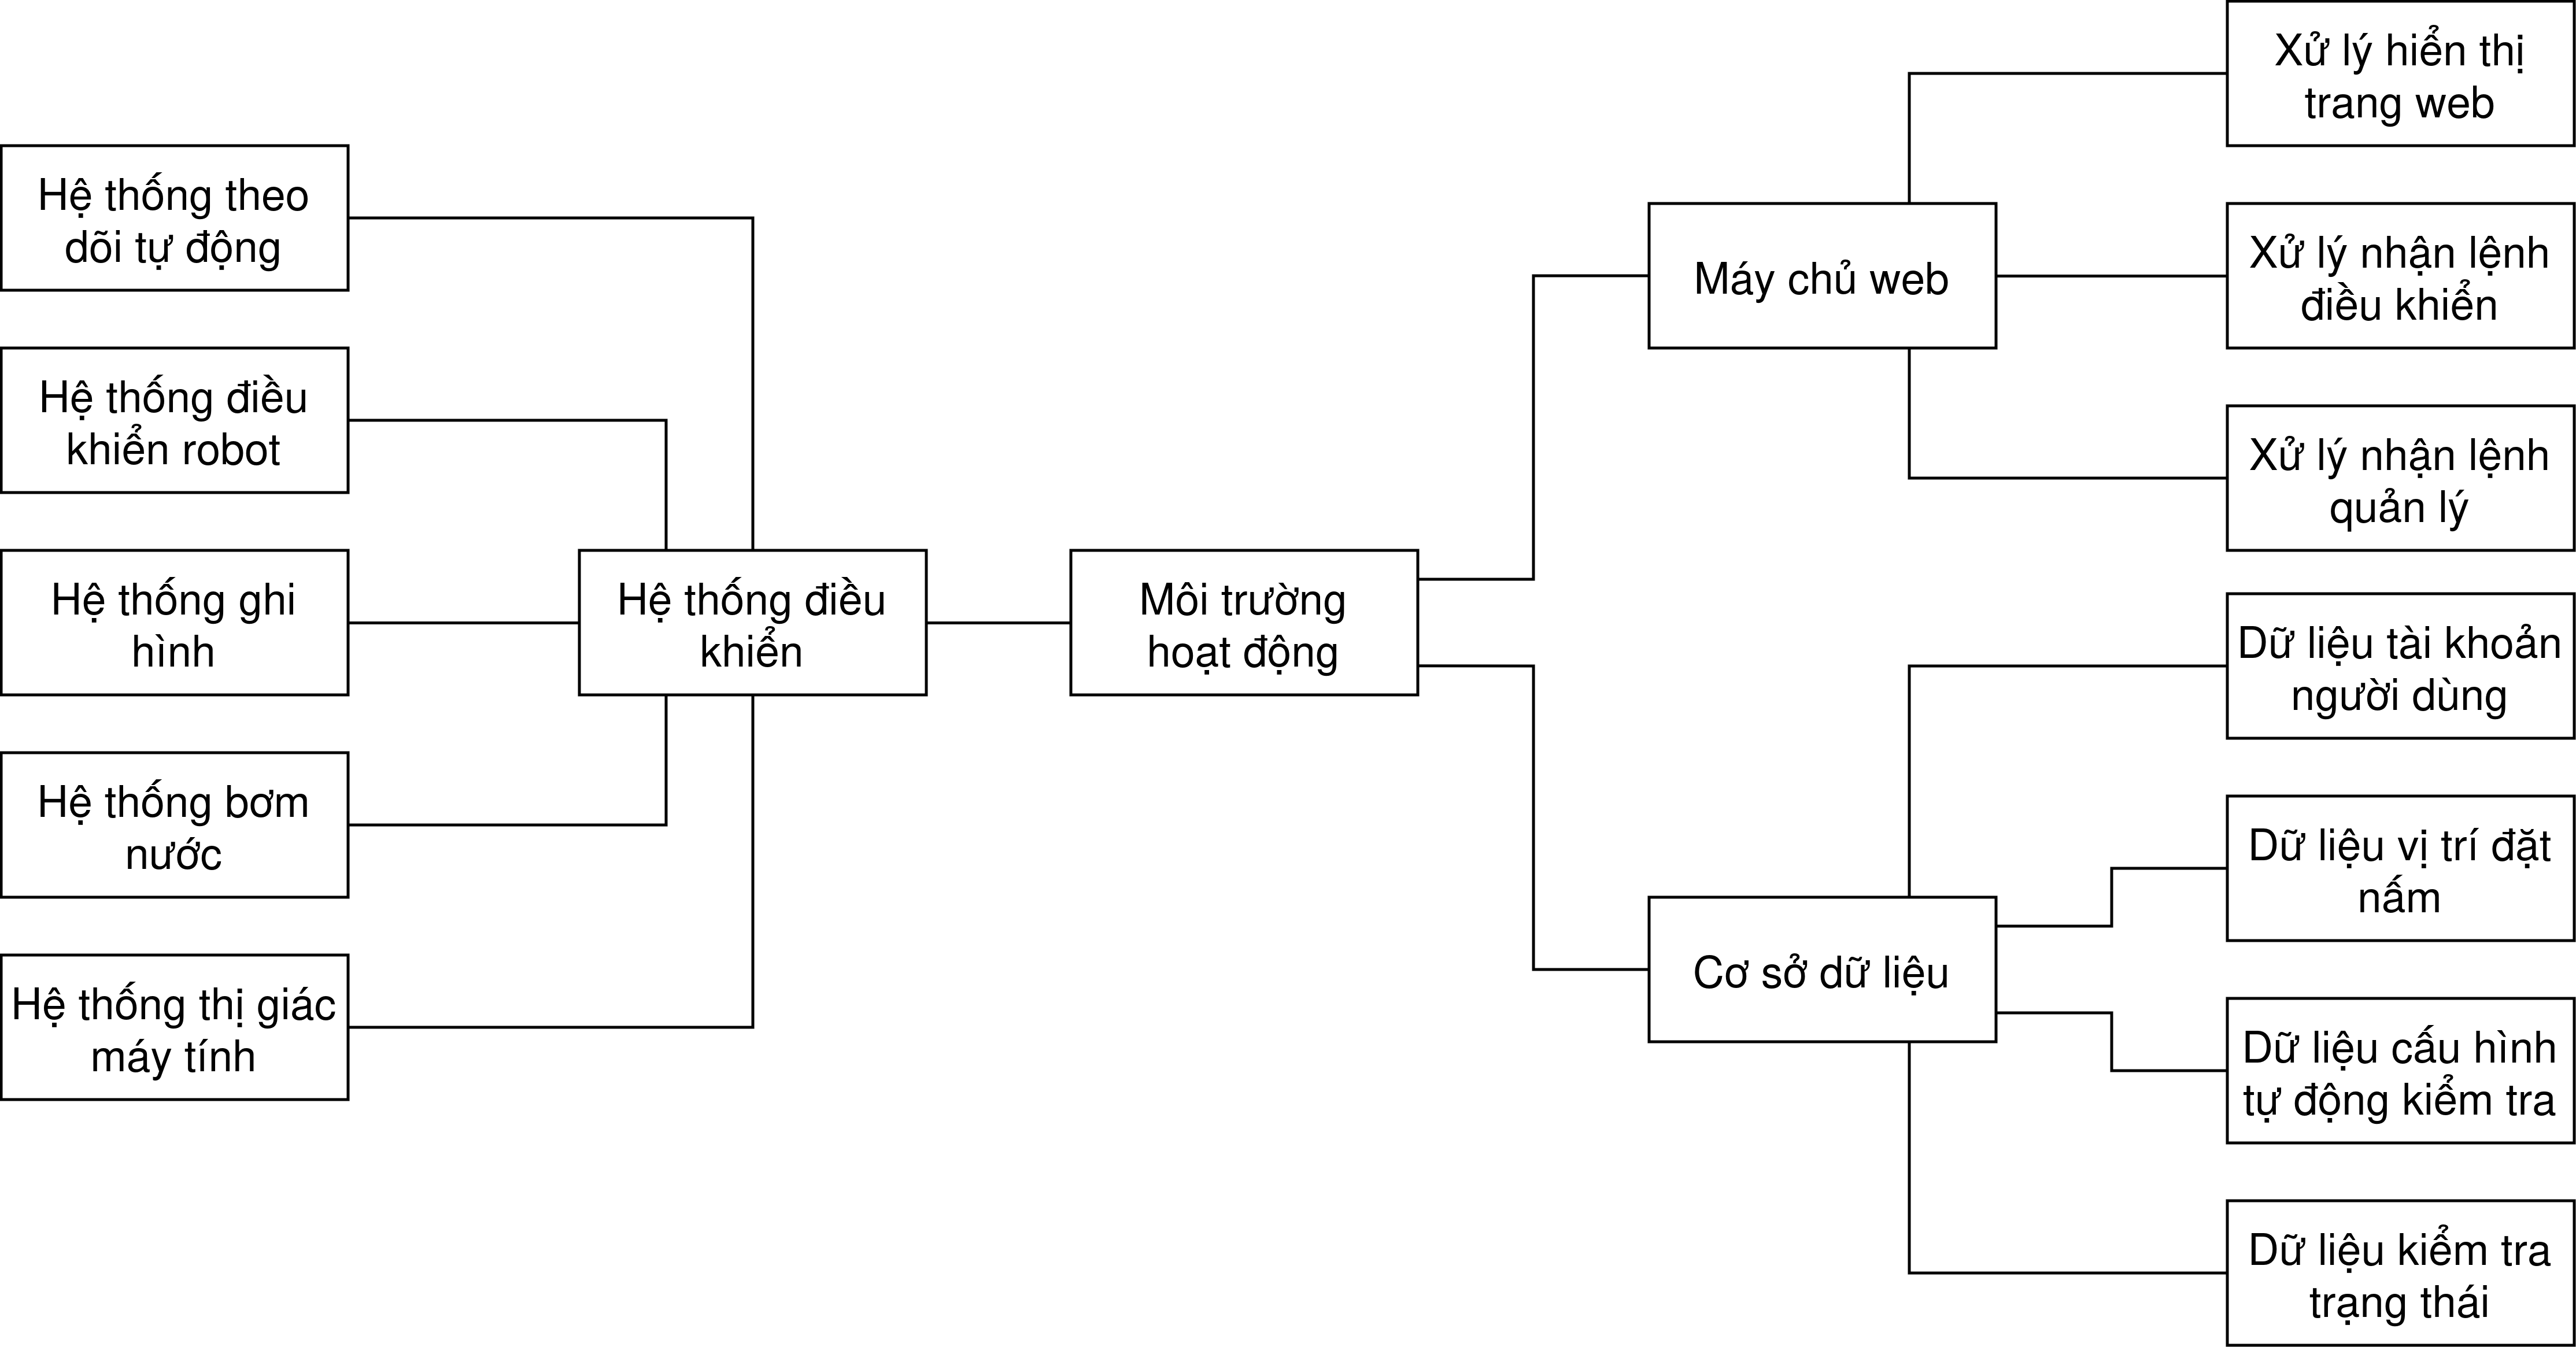
\includegraphics[width=1\linewidth]{images/diagram-objects}
	\caption{Sơ đồ đối tượng trong hệ thống}
	\label{fig:diagram-objects}
\end{figure}

\subsection{Sơ đồ phần cứng}

\begin{figure}[h]
	\centering
	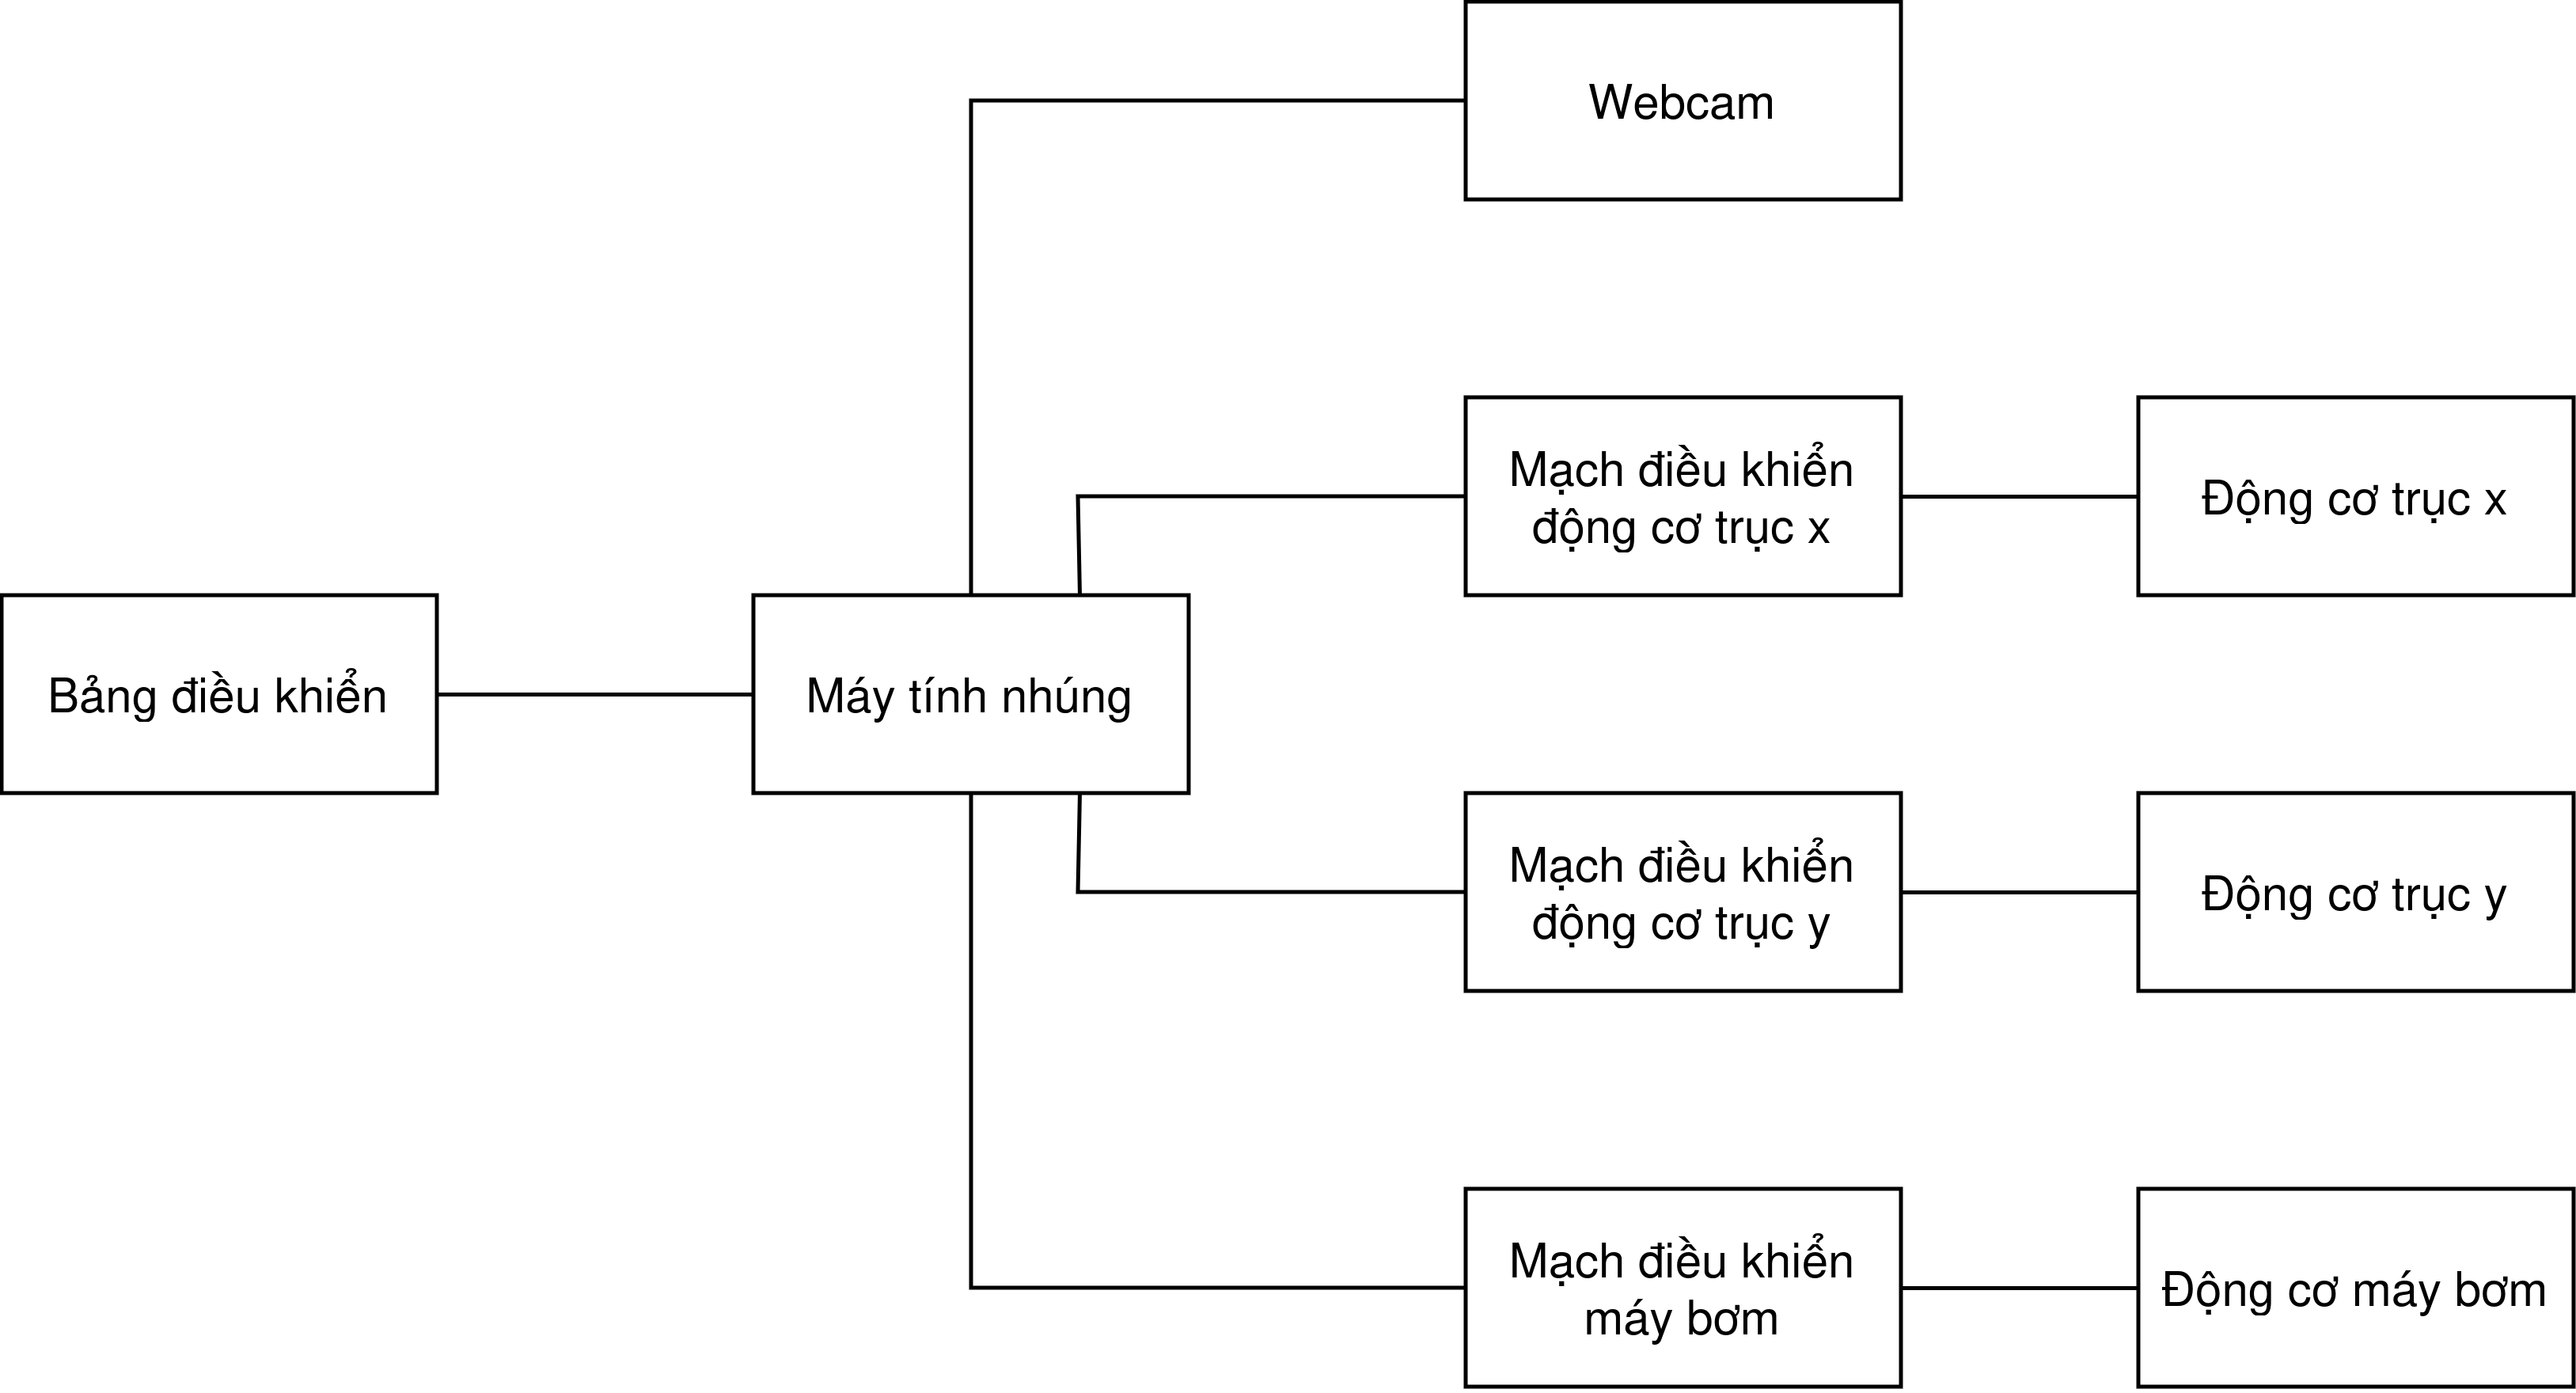
\includegraphics[width=0.7\linewidth]{images/hardware}
	\caption{Sơ đồ phần cứng}
	\label{fig:hardware}
\end{figure}
Hệ thống sử dụng webcam để ghi lại hình ảnh nấm, máy bơm để tưới nước cung cấp độ ẩm cho nấm. Các thiết bị này được di chuyển tới từng vị trí đặt nấm thông qua hai động cơ bước.

Trung tâm của hệ thống là máy tính nhúng giúp điều khiển toàn bộ hoạt động của hệ thống và là nơi lưu trữ dữ liệu. Bảng điều khiển cung cấp giao diện cho người dùng tương tác với hệ thống.





\subsection{Sơ đồ hợp tác}
\subsubsection{Sơ đồ yêu cầu hiển thị trang web}

Các yêu cầu theo dõi hệ thống, truy cập các trang quản lý được gọi chung là yêu cầu hiển thị, được mô tả trong biểu đồ hình \ref{fig:collab-show}.
\begin{figure}[h]
	\centering
	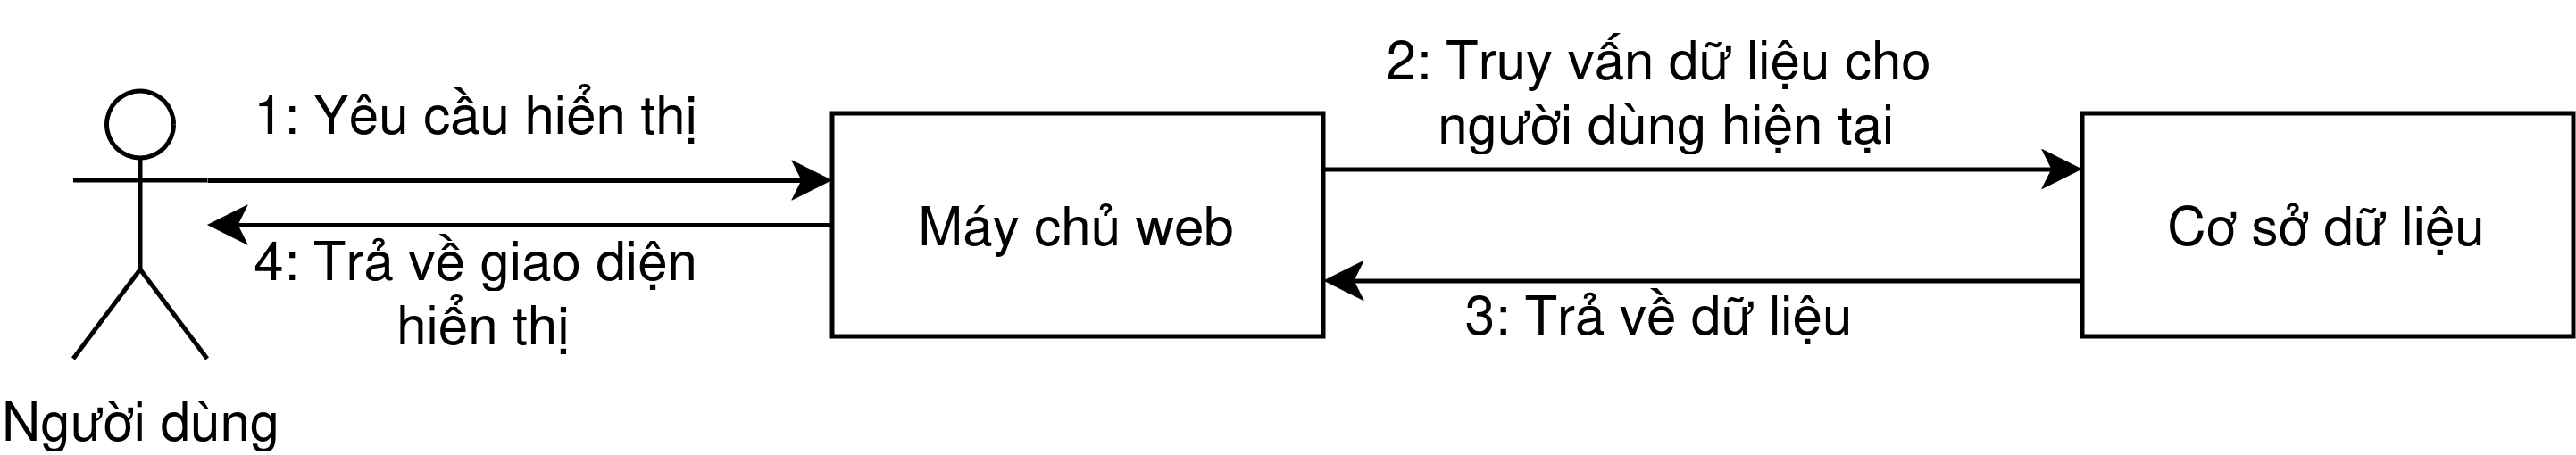
\includegraphics[width=0.8\linewidth]{images/collab-show}
	\caption{Sơ đồ yêu cầu hiển thị trang web}
	\label{fig:collab-show}
\end{figure}

\subsubsection{Sơ đồ yêu cầu cập nhật dữ liệu}
Các yêu cầu cập nhật, xóa bỏ trong quản lý người dùng, quản lý vị trí được gọi chung là yêu cầu cập nhật dữ liệu được mô tả trong hình \ref{fig:collab-update}.
\begin{figure}[H]
	\centering
	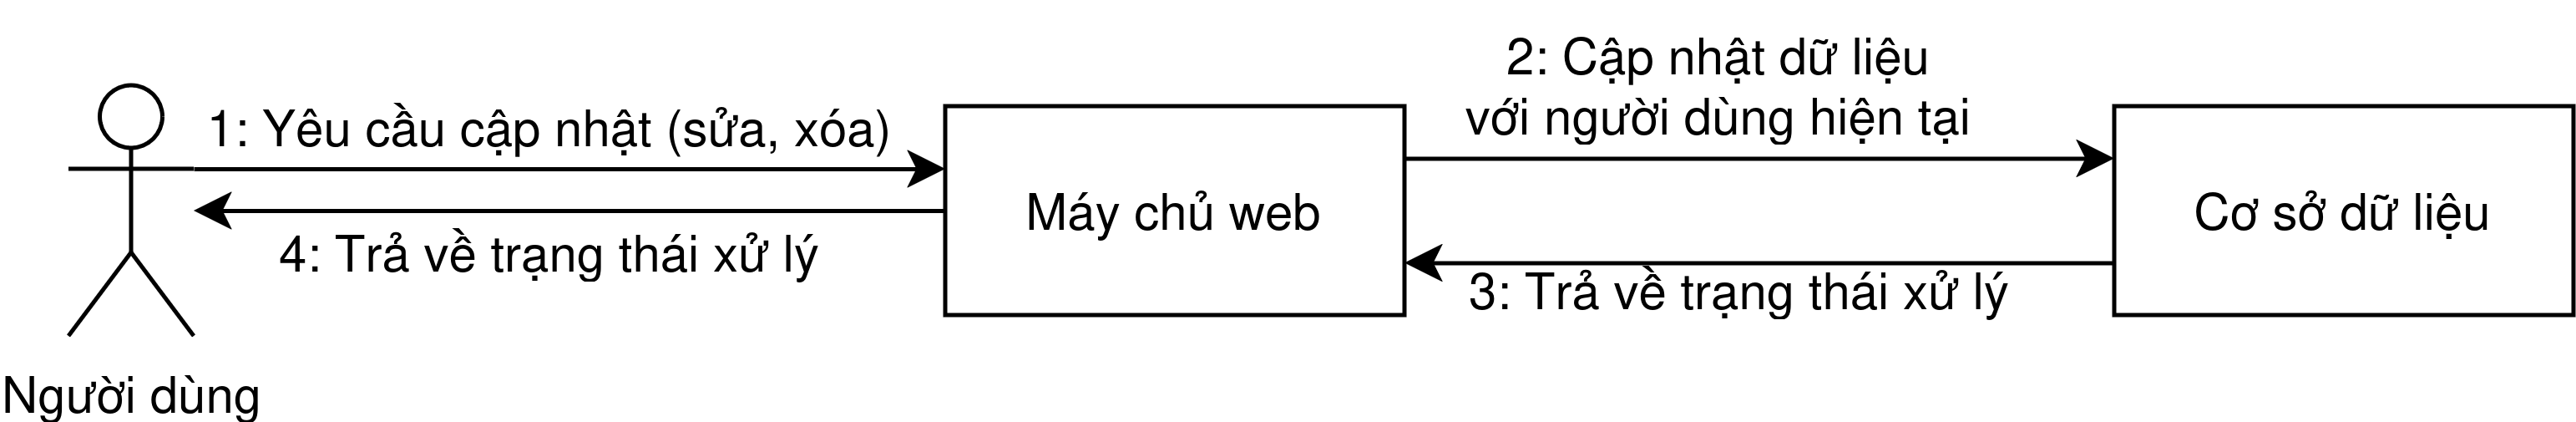
\includegraphics[width=0.8\linewidth]{images/collab-update}
	\caption{Sơ đồ yêu cầu cập nhật dữ liệu}
	\label{fig:collab-update}
\end{figure}

\subsubsection{Sơ đồ yêu cầu điều khiển}
Các yêu cầu kiểm tra, tưới nước từ người dùng được gọi chung là yêu cầu điều khiển, được mô tả trong hình \ref{fig:collab-control}.
\begin{figure}[h]
	\centering
	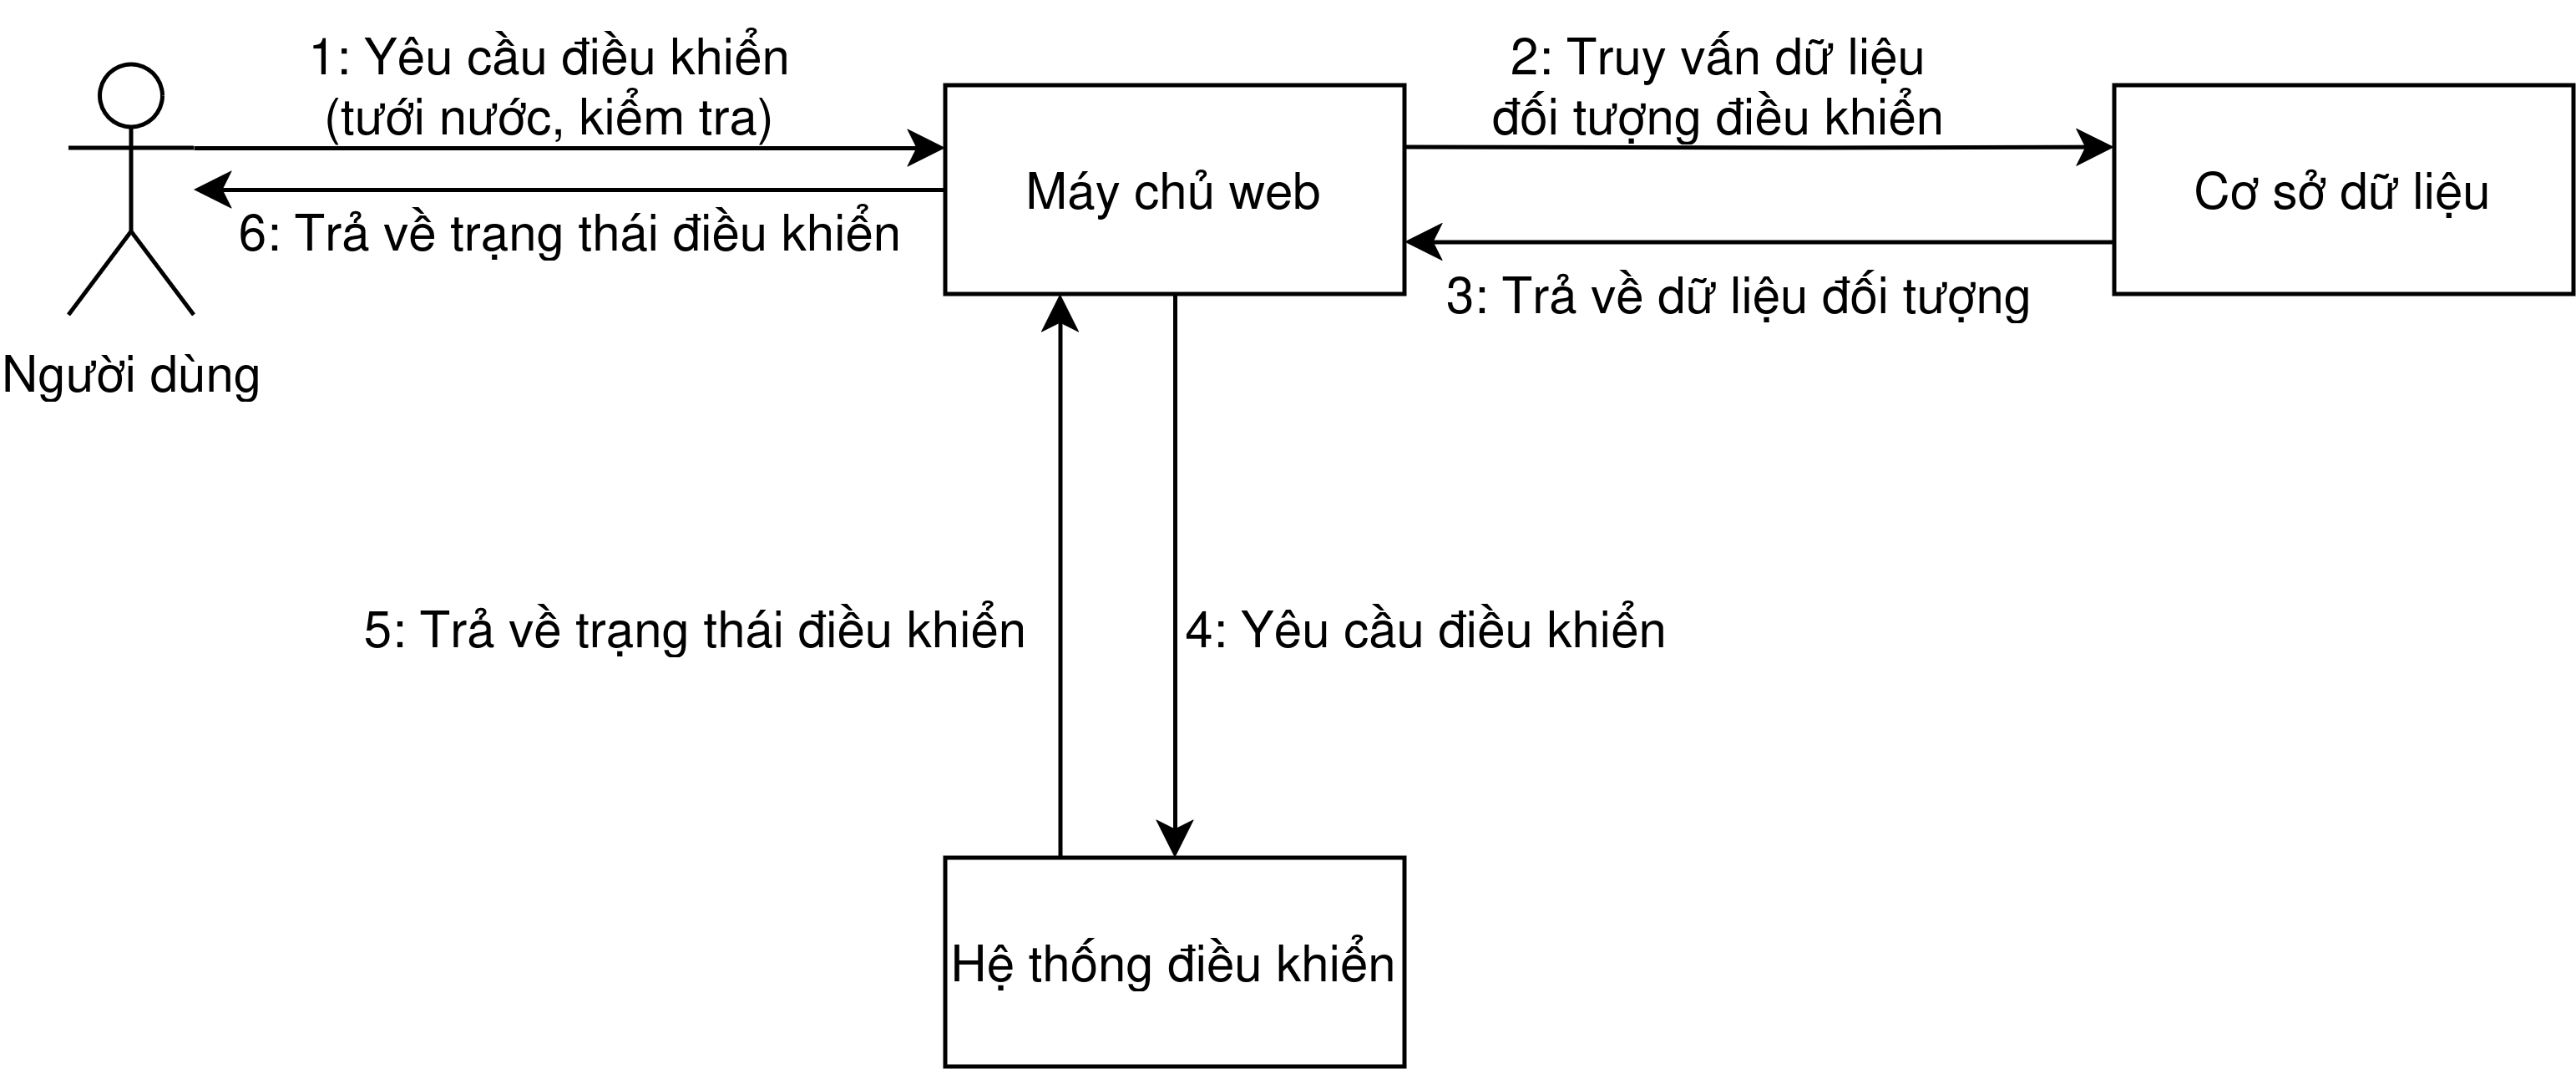
\includegraphics[width=0.8\linewidth]{images/collab-control}
	\caption{Sơ đồ yêu cầu điều khiển}
	\label{fig:collab-control}
\end{figure}

\subsubsection{Sơ đồ theo dõi tự động}
Hoạt động của hệ thống theo dõi tự động được mô tả trong hình \ref{fig:collab-automation}.
\begin{figure}[h]
	\centering
	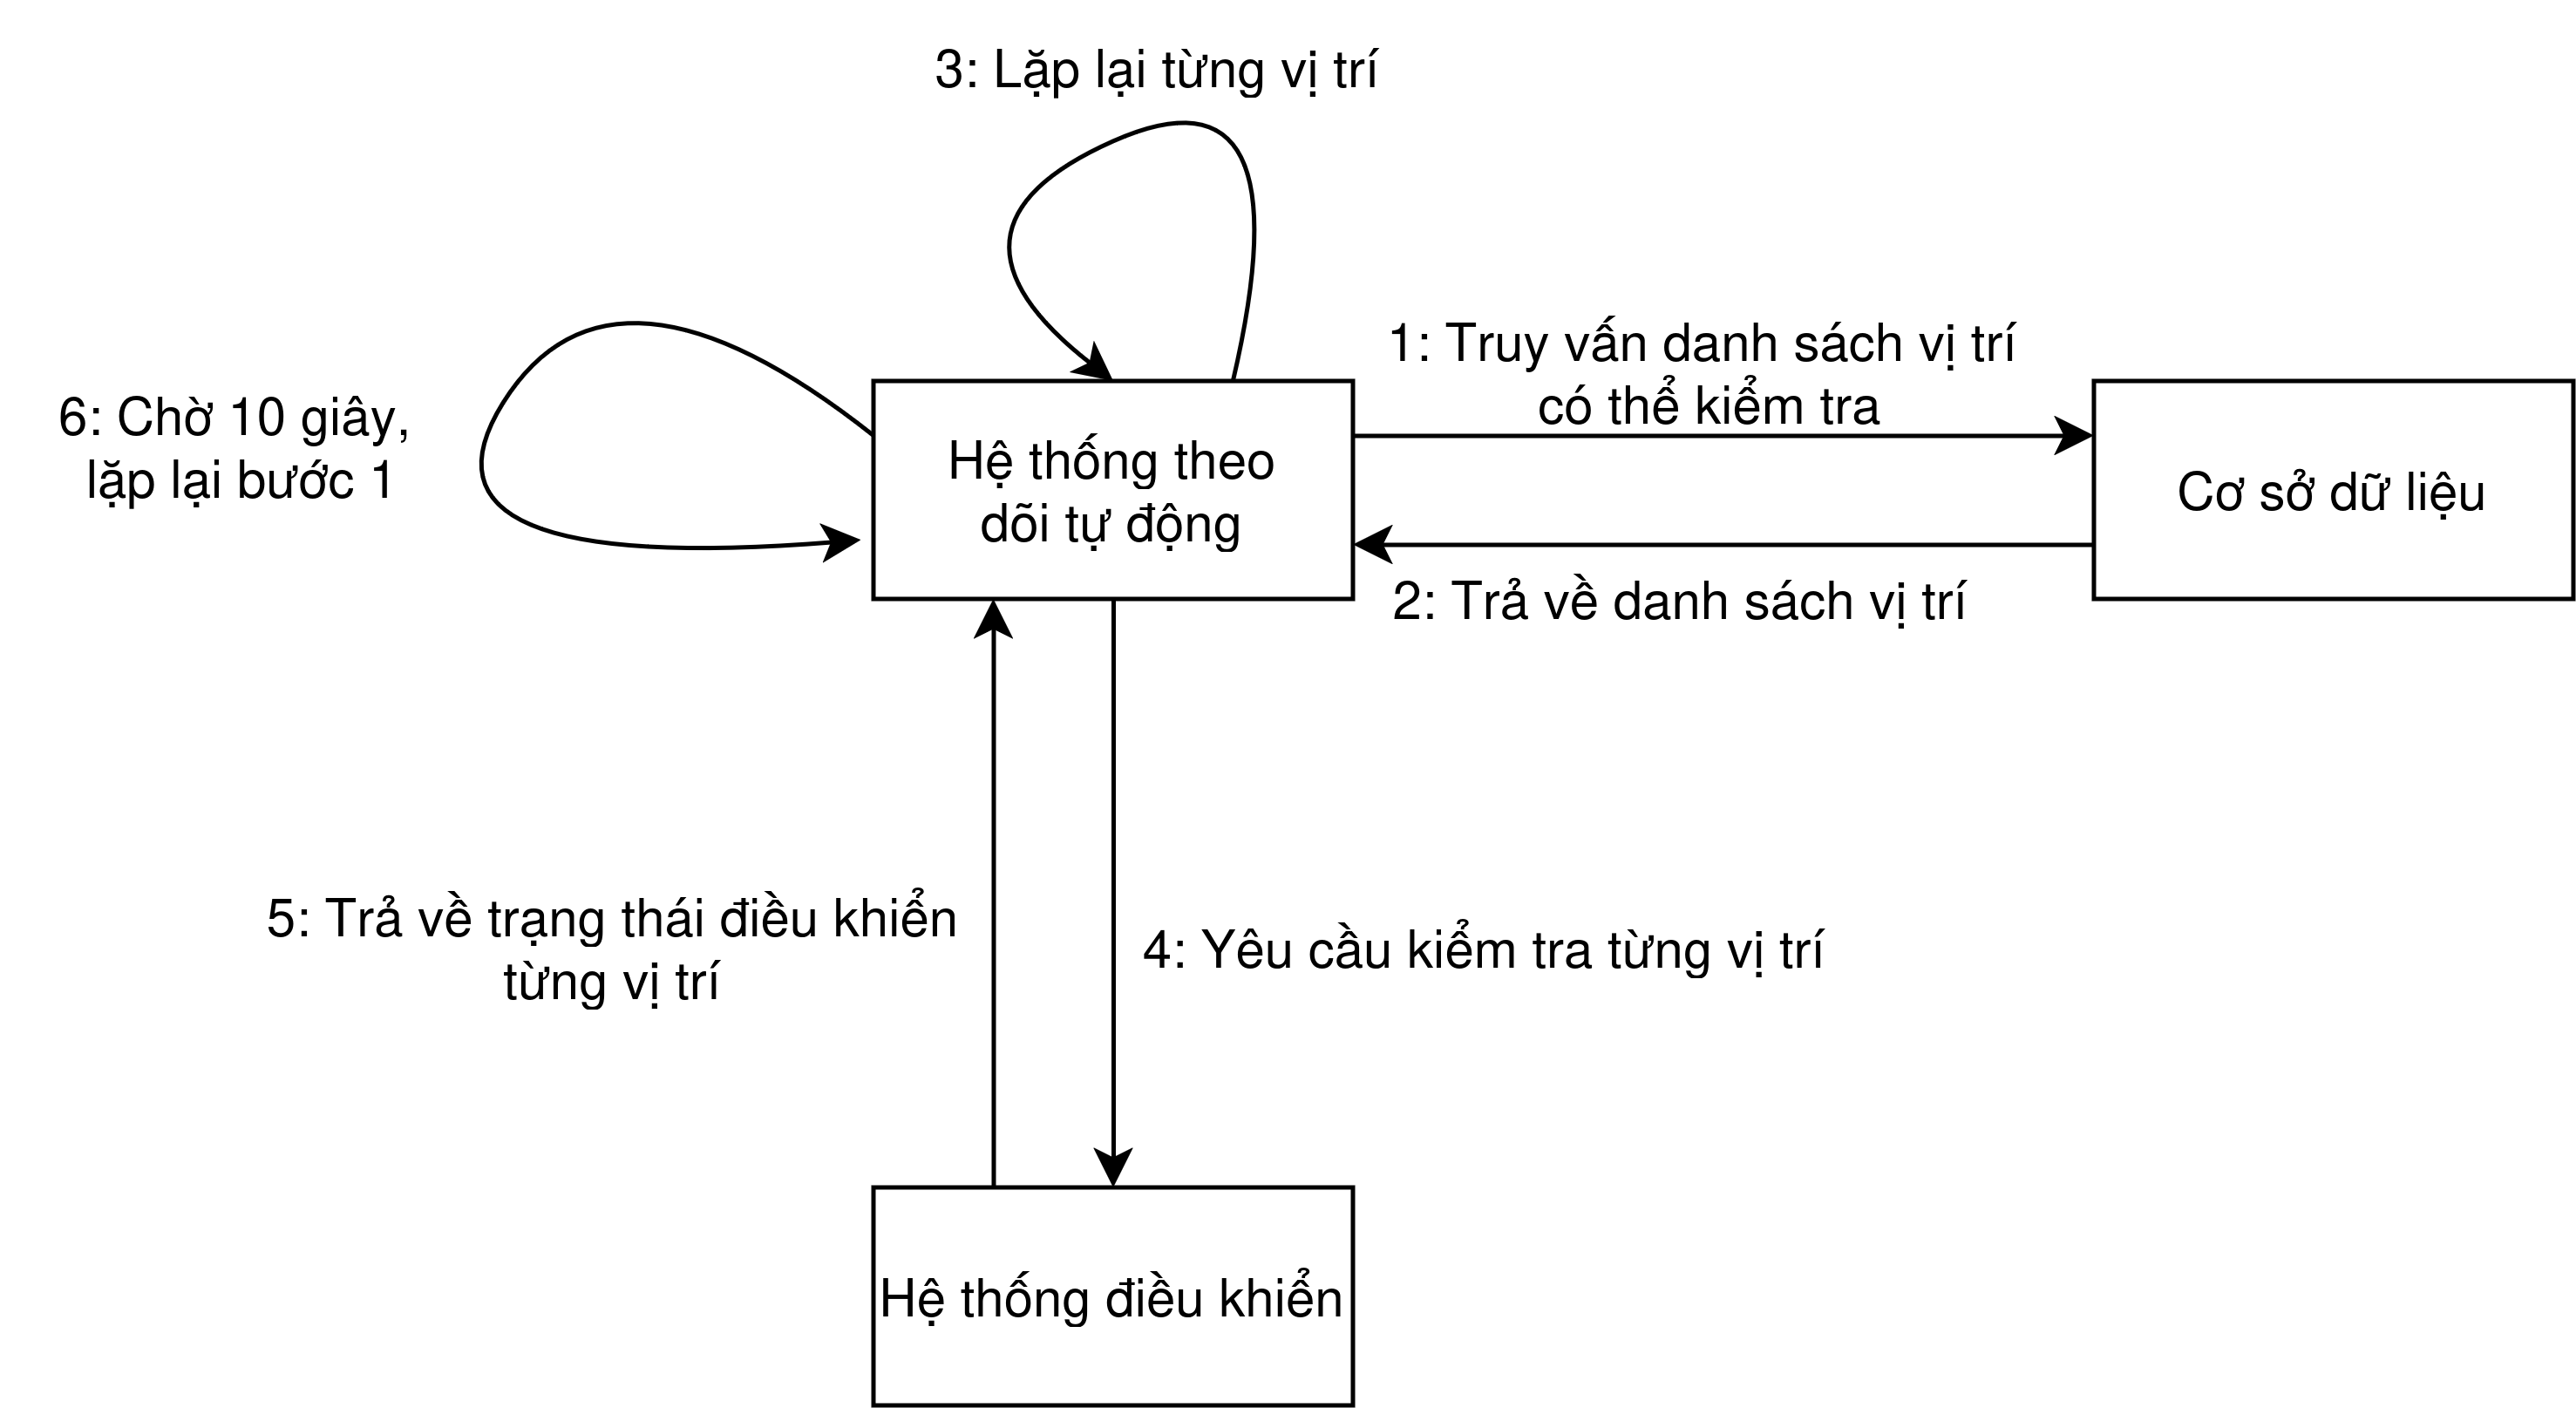
\includegraphics[width=0.8\linewidth]{images/collab-automation}
	\caption{Sơ đồ theo dõi tự động}
	\label{fig:collab-automation}
\end{figure}

\subsubsection{Sơ đồ điều khiển chi tiết}

\begin{figure}[H]
	\centering
	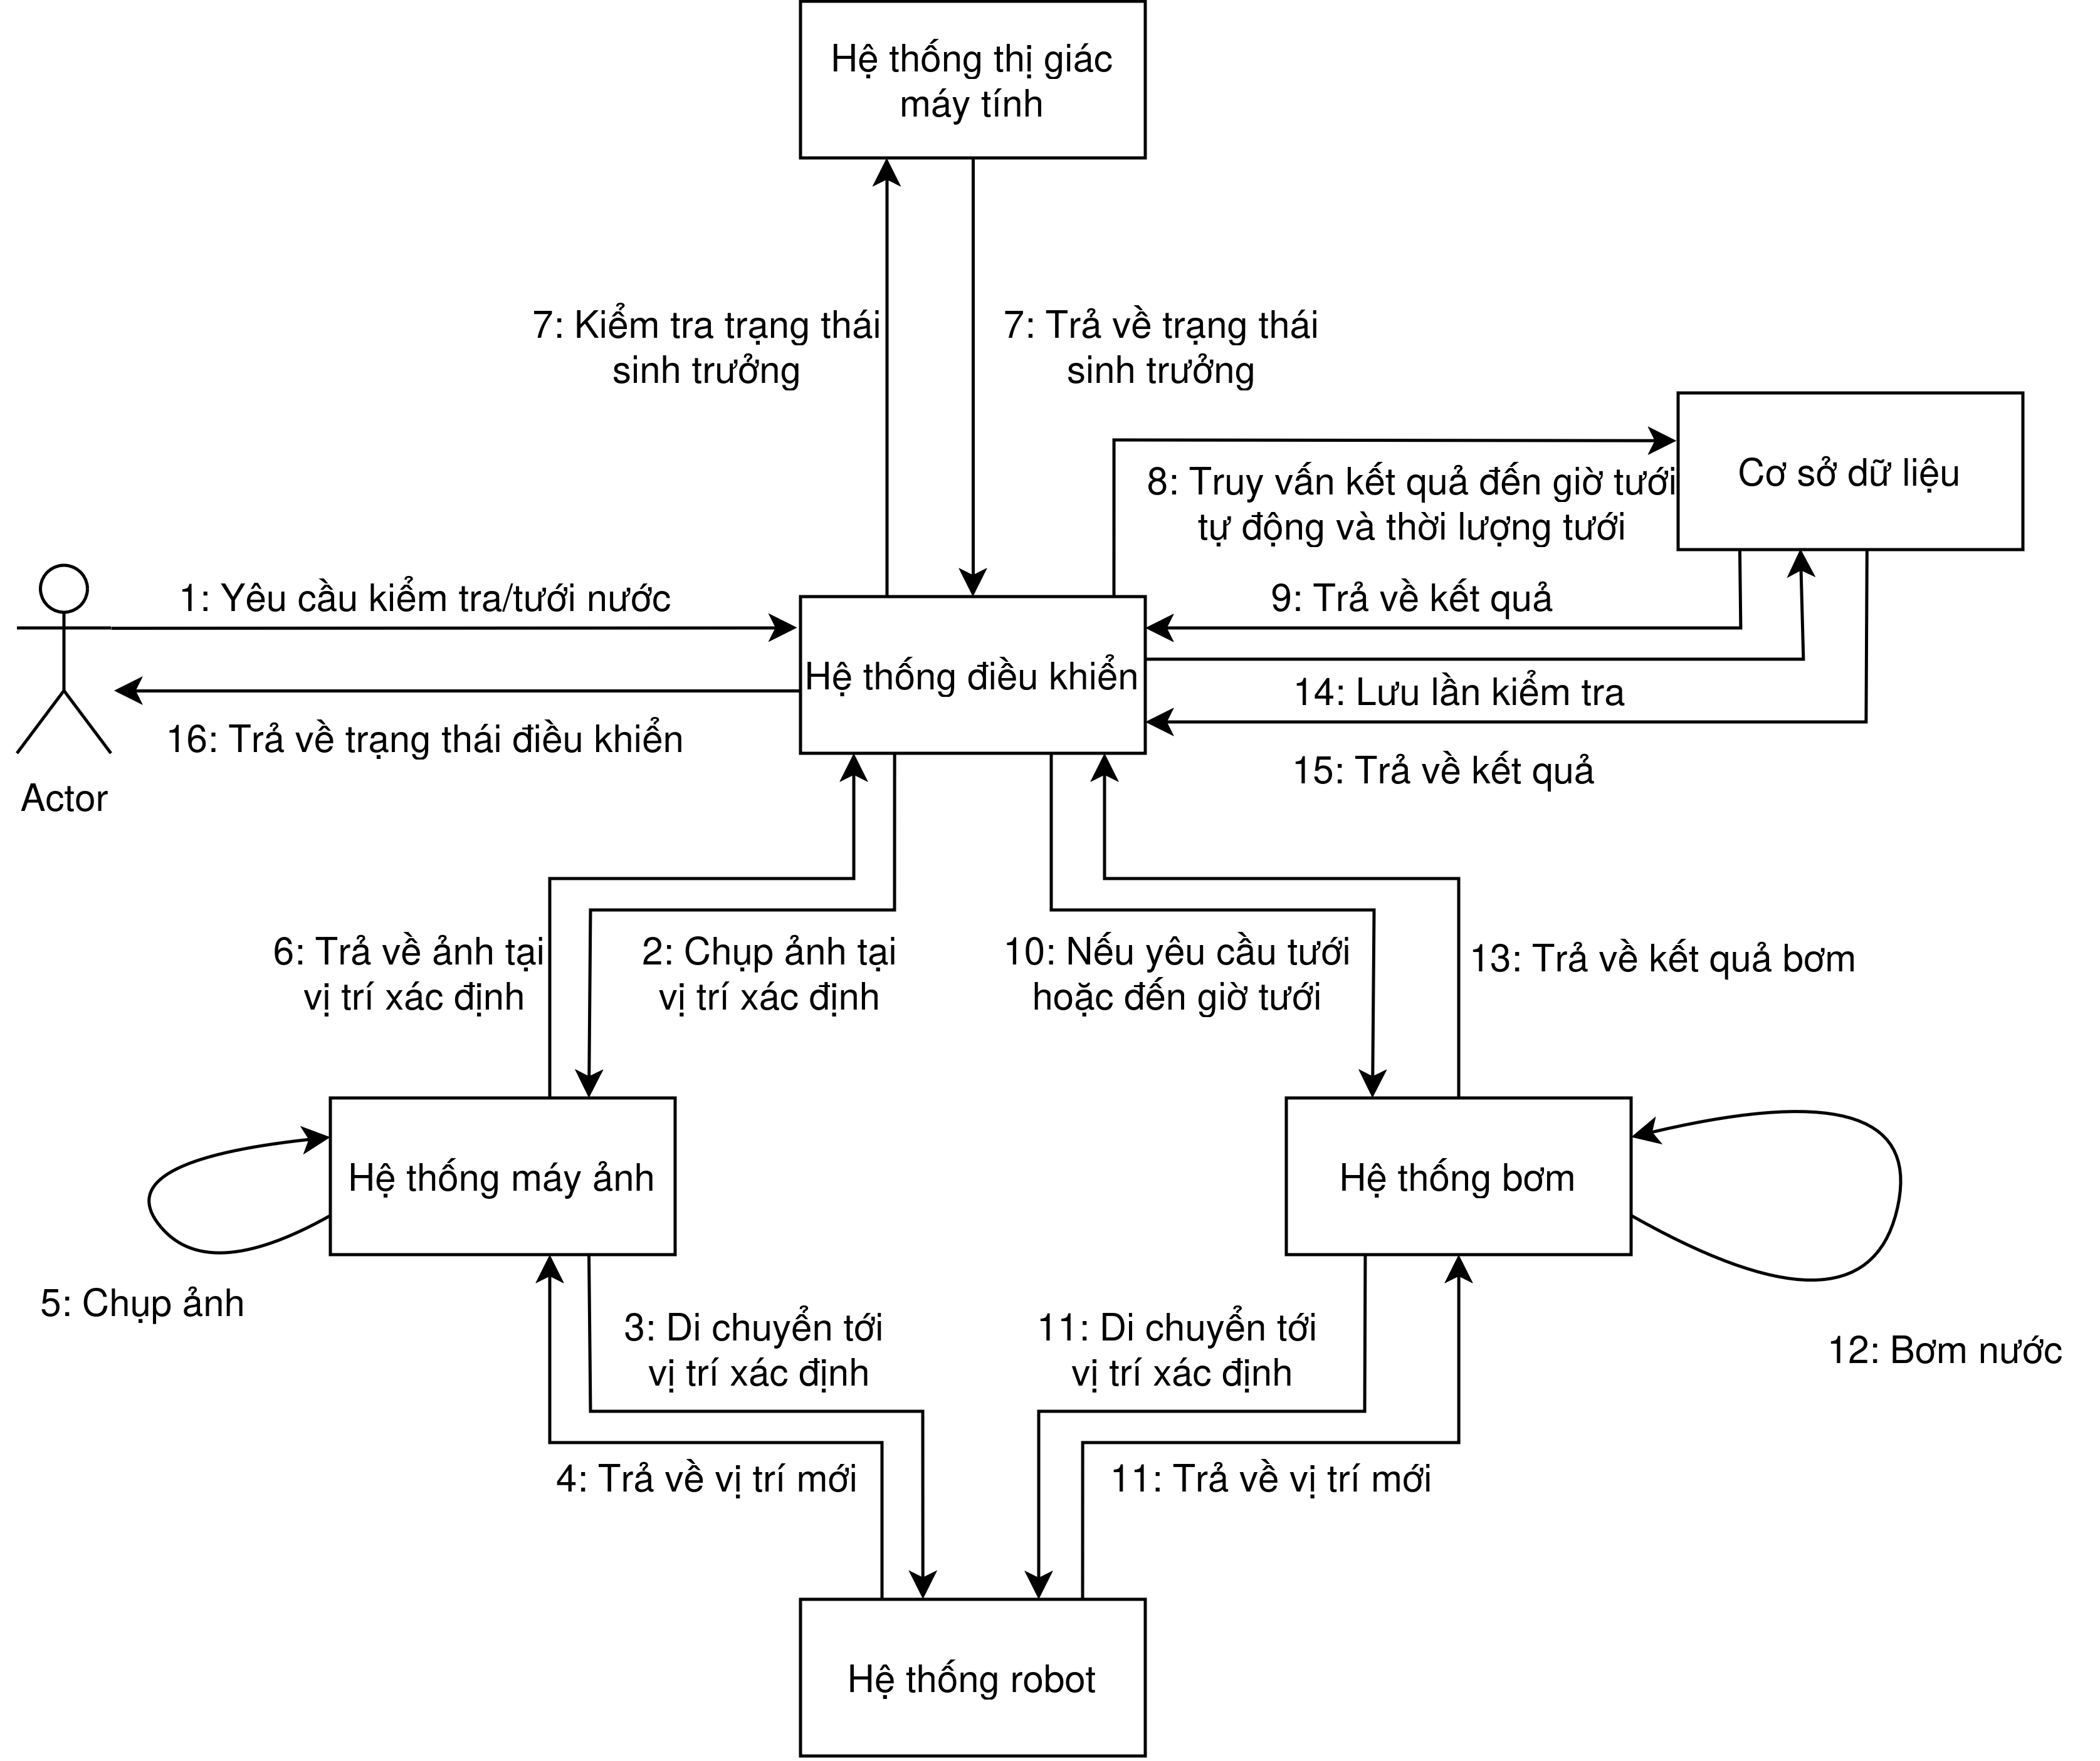
\includegraphics[width=0.8\linewidth]{images/collab-control-detail}
	\caption{Sơ đồ yêu cầu điều khiển chi tiết}
	\label{fig:collab-control-detail}
\end{figure}

Hoạt động của hệ thống điều khiển được mô tả chi tiết trong hình \ref{fig:collab-control-detail}. Tại đây, hệ thống điều khiển gửi lệnh tới hệ thống máy ảnh và hệ thống bơm, hai hệ thống này thực hiện di chuyển tới vị trí tương ứng thông qua hệ thống robot. Dữ liệu hình ảnh được xử lý thông qua hệ thống thị giác máy tính và được xử lý, lưu lại trong cơ sở dữ liệu nhờ hệ thống điều khiển.



\section{Xây dựng tập dữ liệu và huấn luyện mô hình}

\subsection{Thu thập dữ liệu}

Nấm sò trắng là loại nấm phổ biến, được sử dụng nhiều trong các bữa ăn với khả năng chống chịu tốt với điều kiện thời tiết, cho khả năng thu hoạch nhiều lần sau mỗi một tuần. Với số lượng nấm trồng thử là 20 bịch phôi, sau 2 tháng, số lượng nấm thu được tối đa là 160. Số nấm này được lấy hình ảnh phục vụ quá trình thử nghiệm hệ thống.

Ngoài dữ liệu hình ảnh thu được trong thực tế trồng nấm, nguồn ảnh huấn luyện có thể thu thập từ nguồn mạng xã hội.

Trong quá trình trồng thử nghiệm nấm để lấy dữ liệu hình ảnh, nấm được tưới nước với các mức độ khác nhau và hình ảnh được quay phim lại hằng ngày giúp thu được nguồn dữ liệu hình ảnh đa dạng nhất có thể.

Roboflow là một nền tảng hỗ trợ tốt cho việc chuẩn bị dữ liệu huấn luyện. Dữ liệu huấn luyện có thể được tải lên Roboflow dưới dạng ảnh hoặc dạng video sau đó chuyển thành từng khung hình.


\subsection{Chuẩn bị dữ liệu huấn luyện}

Sau khi chuẩn bị dữ liệu huấn luyện, thực hiện gán nhãn cho từng vật thể sử dụng nền tảng Roboflow như trong hình \ref{fig:labelling-interface}. Một số nguyên tắc cần tuân thủ để xây dựng tập dữ liệu mạnh bao gồm:
\begin{itemize}
	\item Tất cả vật thể xuất hiện trong hình đều cần được gán nhãn. Vì mô hình YOLO phát hiện tất cả vật thể trong ảnh, nếu không được gán nhãn đầy đủ, mô hình có thể hoạt động không đúng trong quá trình huấn luyện.
	/
	\item Gán nhãn đầy đủ diện tích vật thể, hộp bao cần bao trùm toàn bộ vật thể và hộp bao không được rộng hơn vật thể quá nhiều để tăng tính chính xác cho mô hình.
	
	\item Các vật thể che lấp nhau cũng cần được gán nhãn đầy đủ. Các mô hình phát hiện vật thể nói chung và mô hình YOLO nói riêng sử dụng các mẫu kích thước và hình dạng hộp bao trong quá trình huấn luyện. Vì vậy, khi gán nhãn cho ảnh, những vật thể che lấp nhau nên được gán nhãn cùng các hộp bao như khi chúng không che lấp.
\end{itemize}

\begin{figure}[H]
	\centering
	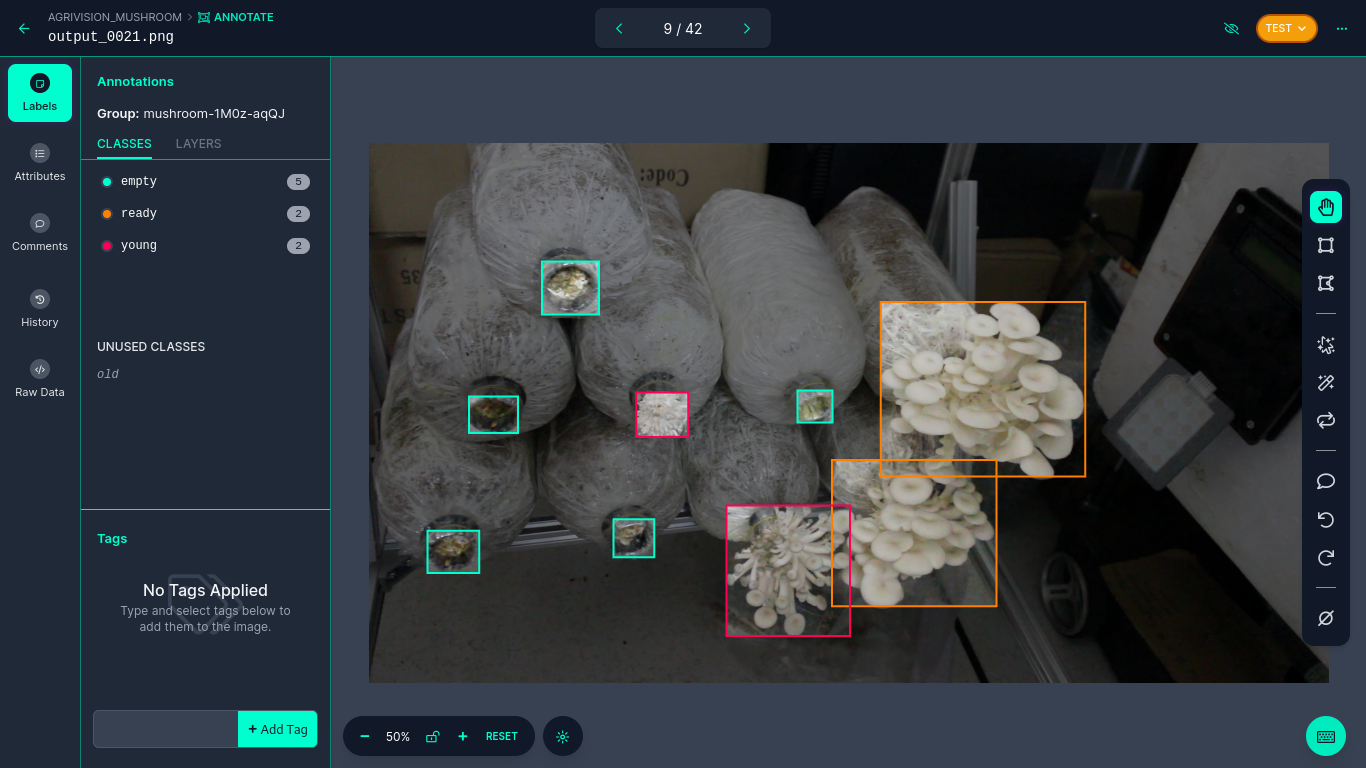
\includegraphics[width=0.7\linewidth]{images/labelling-interface}
	\caption{Giao diện gán nhãn cho nấm}
	\label{fig:labelling-interface}
\end{figure}

\subsection{Gán nhãn ảnh nấm}

Để hệ thống có thể hoạt động với nhiều loại nấm khác nhau, nhãn cho từng giai đoạn phát triển nên được gắn với tên loại nấm. Trong giới hạn của đồ án sử dụng nấm sò trắng, các nhãn chỉ mô tả giai đoạn phát triển của nấm trong các hình \ref{fig:empty}, \ref{fig:young}, \ref{fig:ready}, \ref{fig:old}.

\begin{figure}[h]
	\centering
	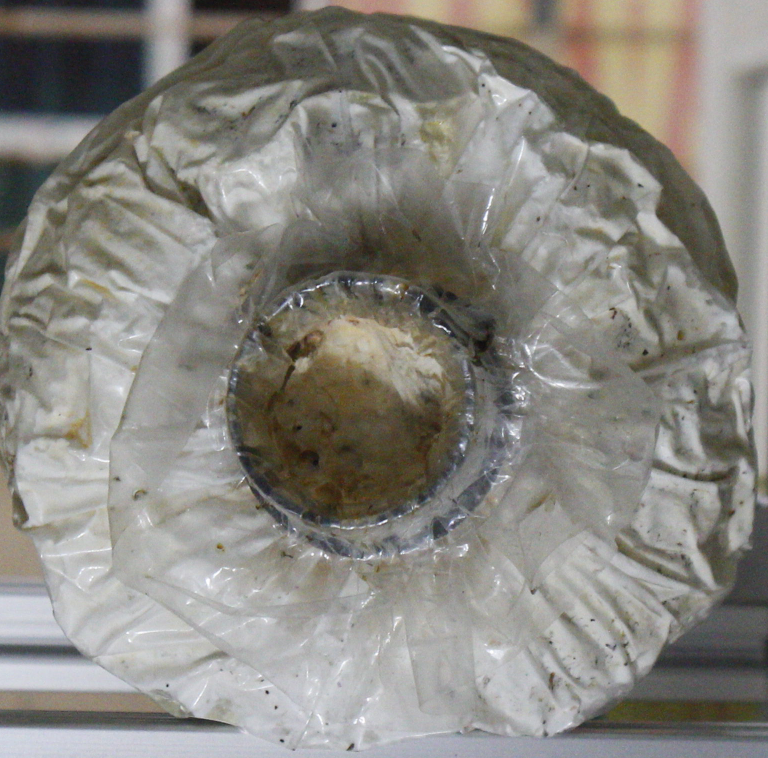
\includegraphics[width=0.4\linewidth]{images/empty}
	\caption{Hình ảnh phôi không có nấm}
	\label{fig:empty}
\end{figure}


Nấm non có thân mọc thẳng về các phía, kích thước tai nấm không lớn hơn thân đáng kể với hình dạng mầu trong hình \ref{fig:young}.

\begin{figure}[H]
    \centering
        \begin{subfigure}{.5\textwidth}
        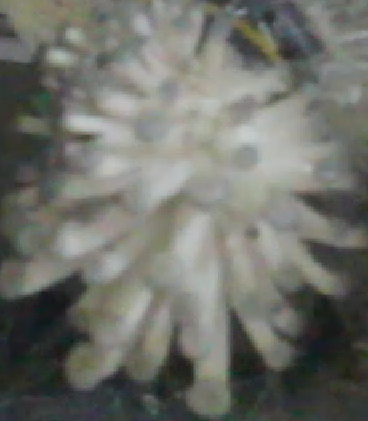
\includegraphics[width=0.8\linewidth]{images/young2.png}
    \end{subfigure}%
    \begin{subfigure}{.5\textwidth}
        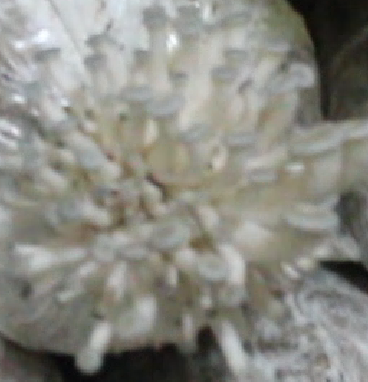
\includegraphics[width=0.8\linewidth]{images/young3.png}
    \end{subfigure}
    \caption{Hình ảnh nấm non}
    \label{fig:young}
\end{figure}

Nấm trưởng thành có tai nấm phát triển, thân nấm uốn cong lên phía trên mô tả trong hình \ref{fig:ready}.

\begin{figure}[H]
    \centering
        \begin{subfigure}{.5\textwidth}
        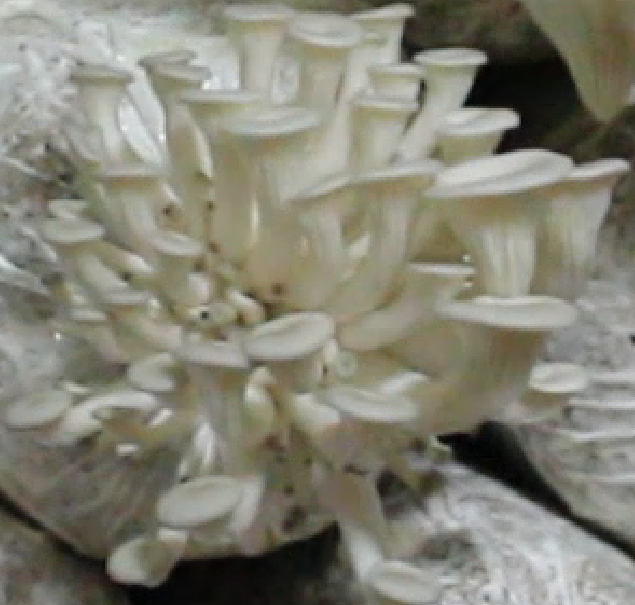
\includegraphics[width=0.8\linewidth]{images/ready1.png}
    \end{subfigure}%
    \begin{subfigure}{.5\textwidth}
        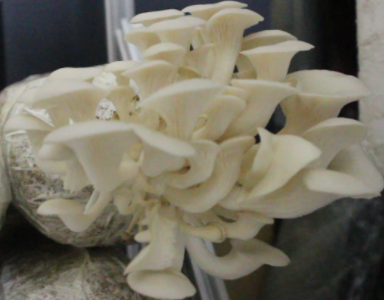
\includegraphics[width=0.8\linewidth]{images/ready3.png}
    \end{subfigure}
    \caption{Hình ảnh nấm trưởng thành, có thể thu hoạch}
    \label{fig:ready}
\end{figure}

Nấm già tai nấm phát triển to có thể bị xoăn lại và chuyển sang màu vàng., thân nấm nhỏ như hình \ref{fig:old}.
\begin{figure}[H]
    \centering
    \begin{subfigure}{.5\textwidth}
        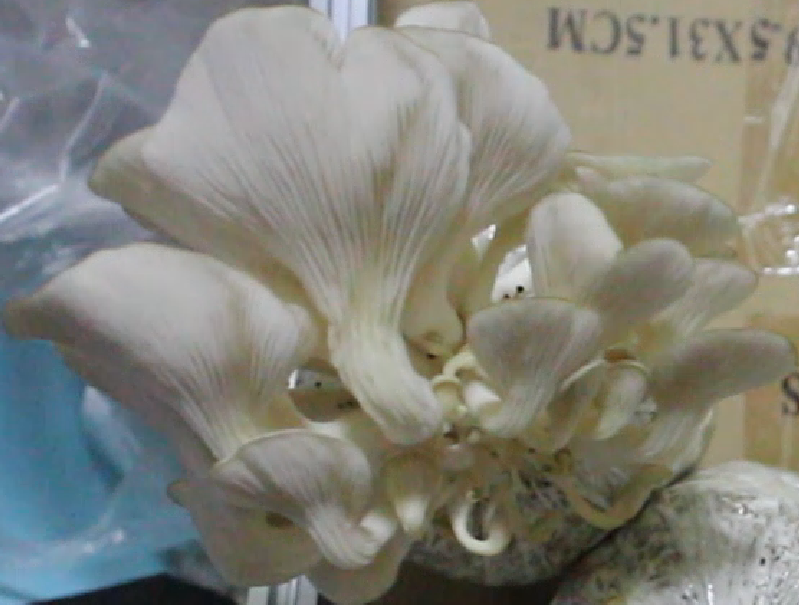
\includegraphics[width=0.85\linewidth]{images/old1.png}
    \end{subfigure}%
    \begin{subfigure}{.5\textwidth}
        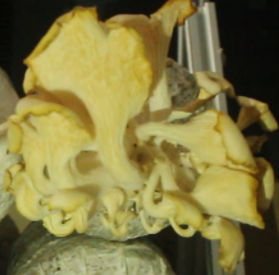
\includegraphics[width=0.85\linewidth]{images/old3.png}
    \end{subfigure}
    \caption{Hình ảnh nấm già}
    \label{fig:old}
\end{figure}

Tổng số hình ảnh được gán nhãn là 852, trong mỗi ảnh có thể có nhiều nấm, trong đó tổng số nấm non là 1135, số nấm trưởng thành là 1274, số nấm già là 526 và số phôi trống là 1622\cite{agrivision_mushroom_dataset}. Số lượng cụ thể cho các tập huấn luyện, tập xác nhận cho mỗi vòng huấn luyện và tập kiểm tra để đánh giá kết quả huấn luyện được thể hiện trong hình \ref{fig:dataset}.

\begin{figure}[H]
	\centering
	\begin{subfigure}{0.8\textwidth}
		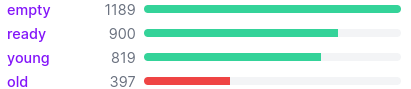
\includegraphics{images/dataset-train}
		\caption{Tập huấn luyện}
	\end{subfigure}
	\begin{subfigure}{0.8\textwidth}
		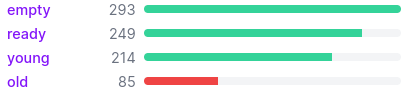
\includegraphics{images/dataset-val}
		\caption{Tập xác nhận}
	\end{subfigure}
	\begin{subfigure}{0.8\textwidth}
		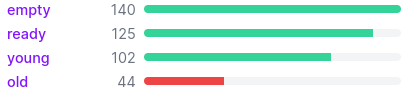
\includegraphics{images/dataset-test}
		\caption{Tập kiểm tra}
	\end{subfigure}
	\caption{Số lượng lớp trong tập dữ liệu}
	\label{fig:dataset}
\end{figure}

Dữ liệu hình ảnh sau khi được gán nhãn cần được xử lý và làm giàu trước khi huấn luyện. Đầu tiên ảnh cần được thay đổi kích thước về kích thước phù hợp với mô hình. Đối với YOLOv8, tỉ lệ kích thước không ảnh hưởng tới kết quả huấn luyện, tuy nhiên, kích thước ảnh huấn luyện cần phù hợp với ảnh sử dụng trong quá trình suy luận. Để phù hợp với ảnh trong quá trình suy luận ảnh sẽ được thay đổi về kích thước 1280x720. Hình ảnh trong tập dữ liệu cũng được làm giàu bằng cách tạo nhiễu.

Sau khi làm giàu, số lượng ảnh được sinh ra là 2086 ảnh. Tập dữ liệu huấn luyện sau khi chuẩn bị đầy đủ sẽ được được tải về và đưa vào huấn luyện. Roboflow hỗ trợ nhiều định dạng khác nhau cho các mạng khác nhau, trong đó có hỗ trợ xuất định dạng tập dữ liệu cho \acrshort{yolo}v8 như hình \ref{fig:export-dataset}.

\begin{figure}[H]
    \centering
    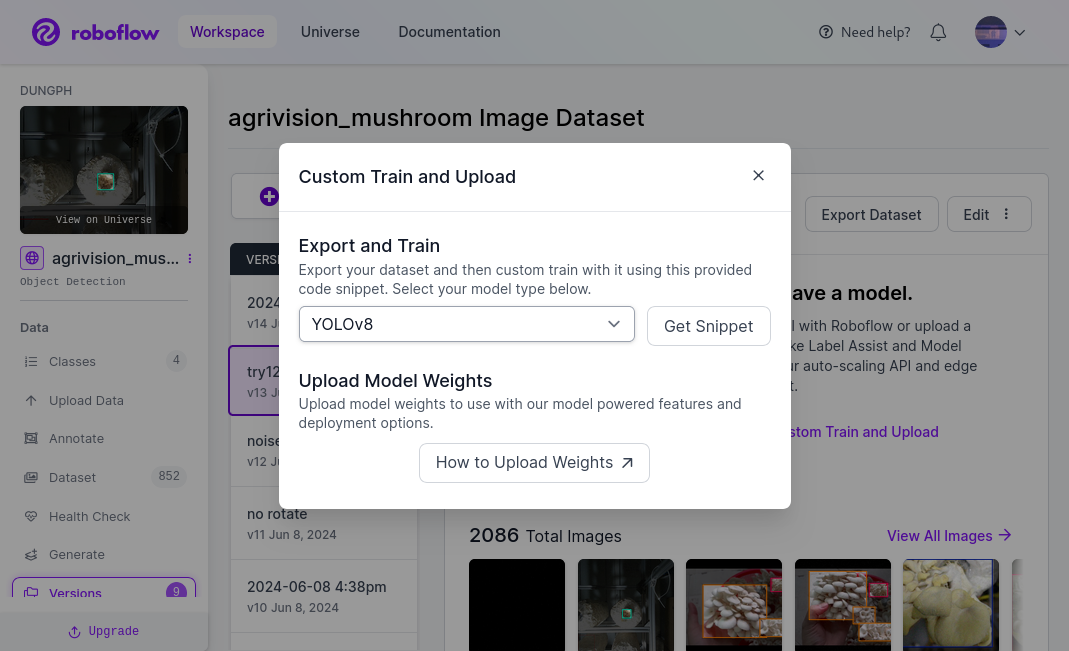
\includegraphics[width=0.85\linewidth]{images/export-dataset.png}
    \caption{Xuất tập dữ liệu huấn luyện}
    \label{fig:export-dataset}
\end{figure}

\subsection{Huấn luyện và đánh giá hiệu suất mô hình}

Ultralytics \cite{yolov8_ultralytics} cung cấp bộ phần mềm hỗ trợ các tác vụ huấn luyện và suy luận sử dụng mô hình \acrshort{yolo} trên các nền tảng hệ điều hành và trên các môi trường trực tuyến như Kaggle. Sử dụng nền tảng Kaggle, do hỗ trợ phần cứng tối ưu, quá trình huấn luyện có thể thực hiện trong thời gian ngắn.

\begin{figure}[h]
	\centering
	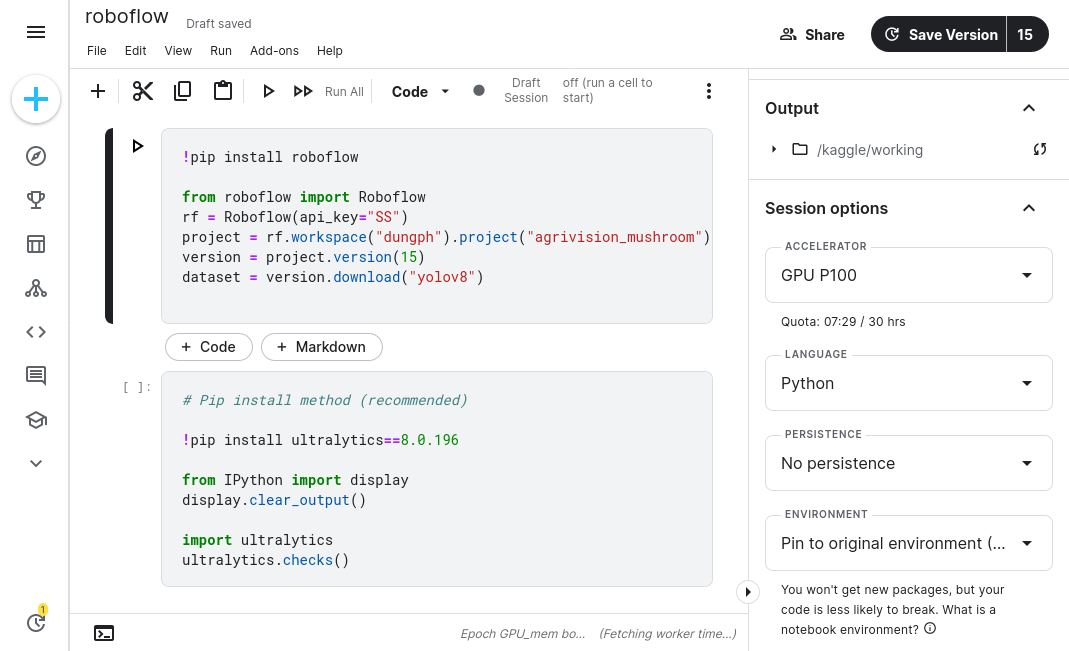
\includegraphics[width=0.9\linewidth]{images/ui-kaggle}
	\caption{Giao diện Kaggle}
	\label{fig:ui-kaggle}
\end{figure}

Các tham số huấn luyện mô hình bao gồm:
\begin{itemize}
	\item Kích thước mô hình YOLO: do số lượng dữ liệu huấn luyện còn nhỏ, mô hình YOLOv8n được sử dụng. Tại đây, chương trình thực hiện tải mô hình đã được huấn luyện từ trước thay vì sử dụng các tham số ngẫu nhiên làm tăng độ phức tạp huấn luyện.
	\item Kích thước hình ảnh (kích thước cạnh dài nhất): sử dụng kích thước 1280px.
	\item Số vòng huấn luyện: khi huấn luyện, nếu chương trình nhận thấy các giá trị mất mát không thể giảm một cách đáng kể, chương trình tự động dừng huấn luyện. Vì vậy, đây là giá trị số vòng huấn luyện tối đa. Giá trị hiện tại epoch = 200.
\end{itemize}

Sau 132 vòng huấn luyện, chương trình tự động dừng lại do không có sự cải thiện đáng kể trong vòng 50 vòng gần nhất. Từ hình \ref{fig:training-result-f1}, mô hình đưa ra kết quả chính xác nhất với hệ số tự tin từ 10\% đến 75\%, hệ số tự tin càng cao càng đưa ra kết quả chính xác trên mỗi dự đoán trong hình \ref{fig:training-result-p} và tỉ lệ phát hiện đúng vật thể bắt đầu giảm rõ rệt khi hệ số tự tin lớn hơn 70\% với biểu đồ trong hình \ref{fig:training-result-r}. Vì vậy, khi triển khai, hệ số tự tin có thể đặt giá trị cao để cho các suy đoán chính xác nhưng không được vượt quá 75\%. Ngược lại, khi cần lượng dự đoán đầy đủ nhất, hệ số tự tin có thể giảm xuống nhưng không giảm quá 10\%

\begin{figure}[H]
    \centering
    \begin{subfigure}{.5\textwidth}
        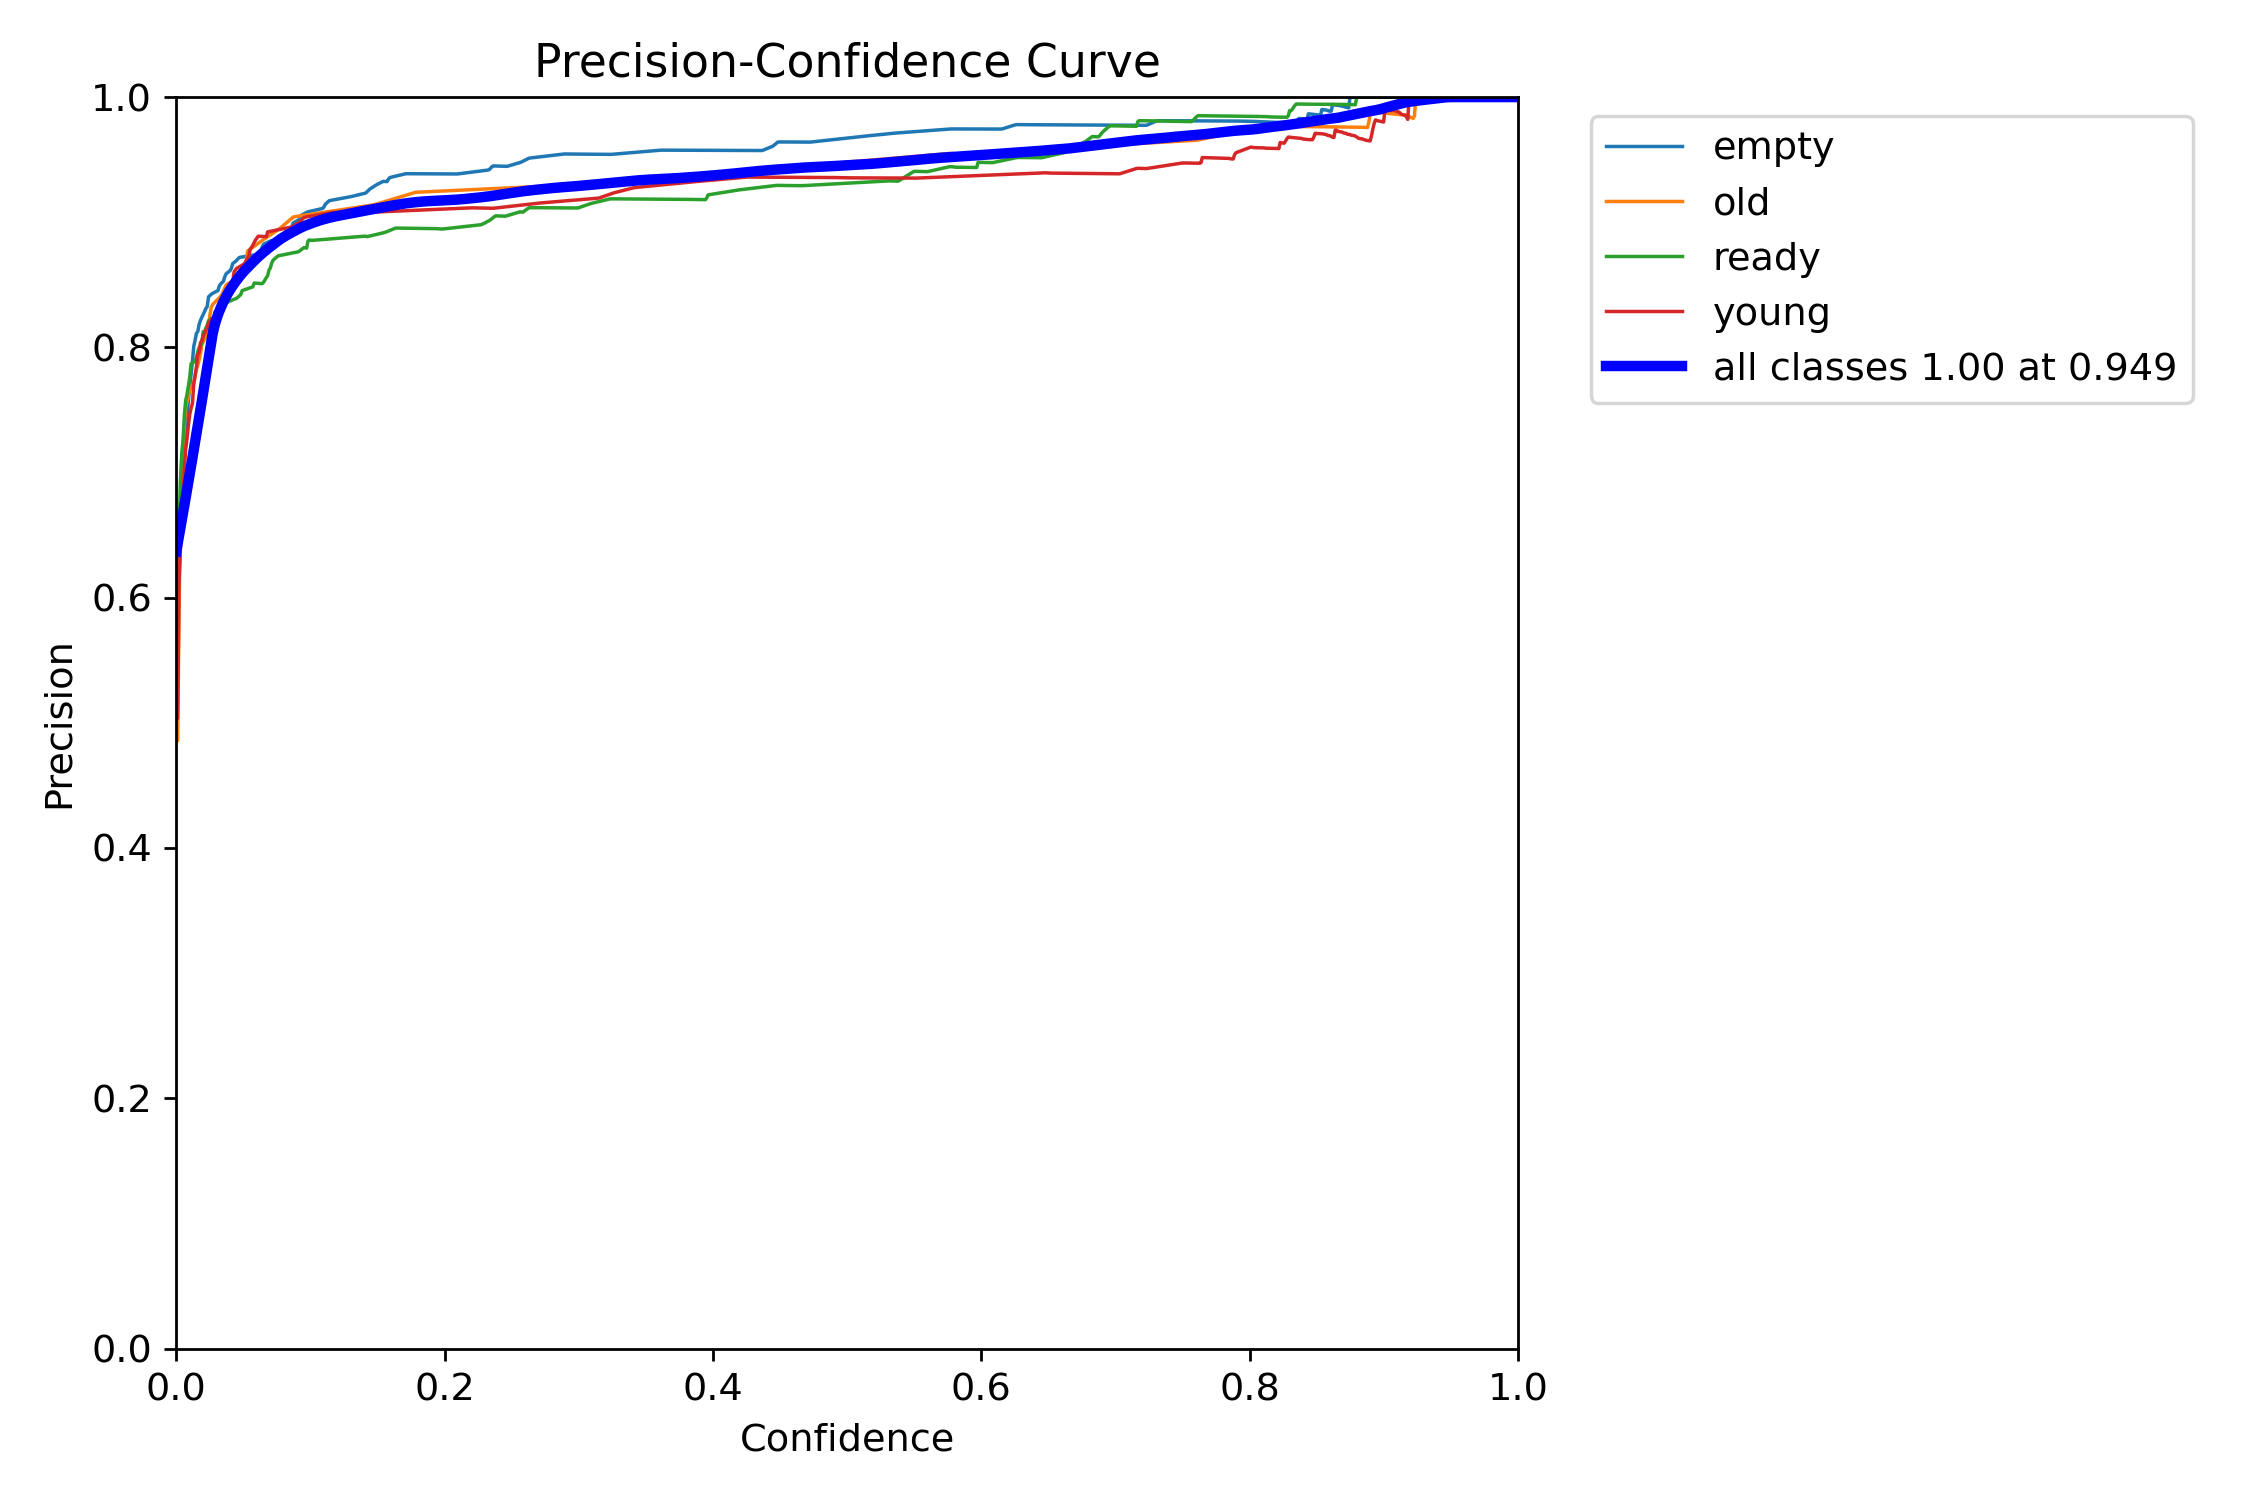
\includegraphics[width=0.95\linewidth]{images/P_curve.png}
    \caption{Đường cong Precision}
    \label{fig:training-result-p}

    \end{subfigure}%
    \begin{subfigure}{.5\textwidth}
        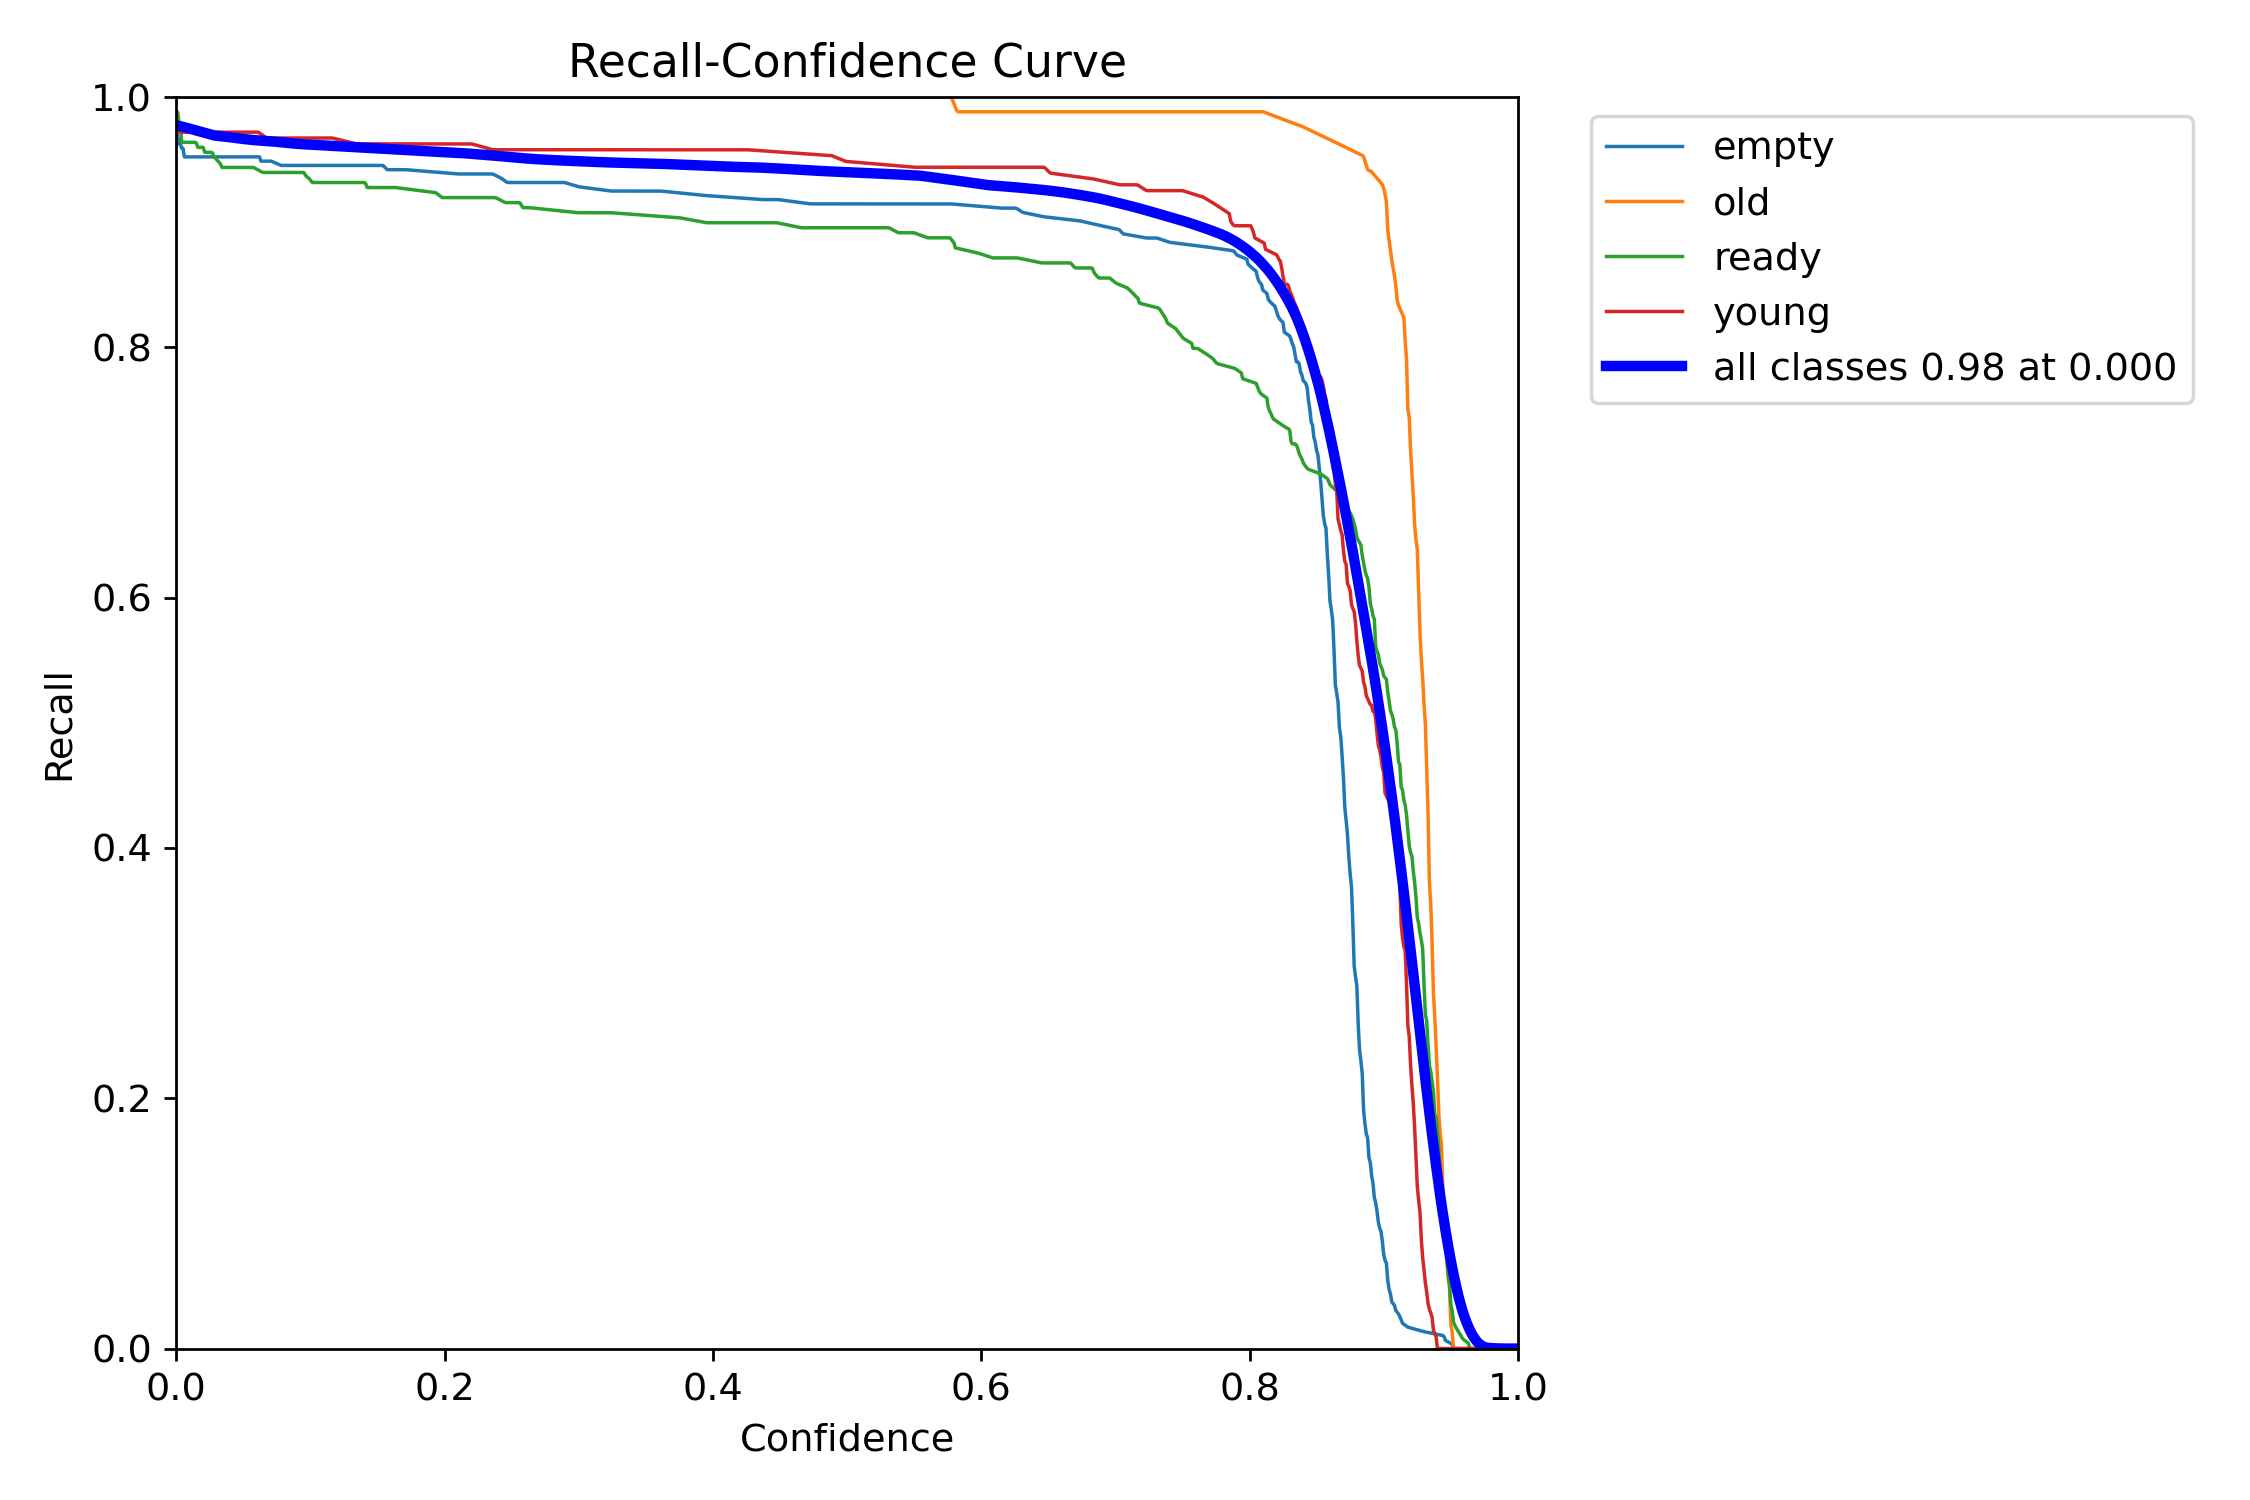
\includegraphics[width=0.95\linewidth]{images/R_curve.png}
    \caption{Đường cong Recall}
    \label{fig:training-result-r}
    \end{subfigure}
    \begin{subfigure}{.5\textwidth}
        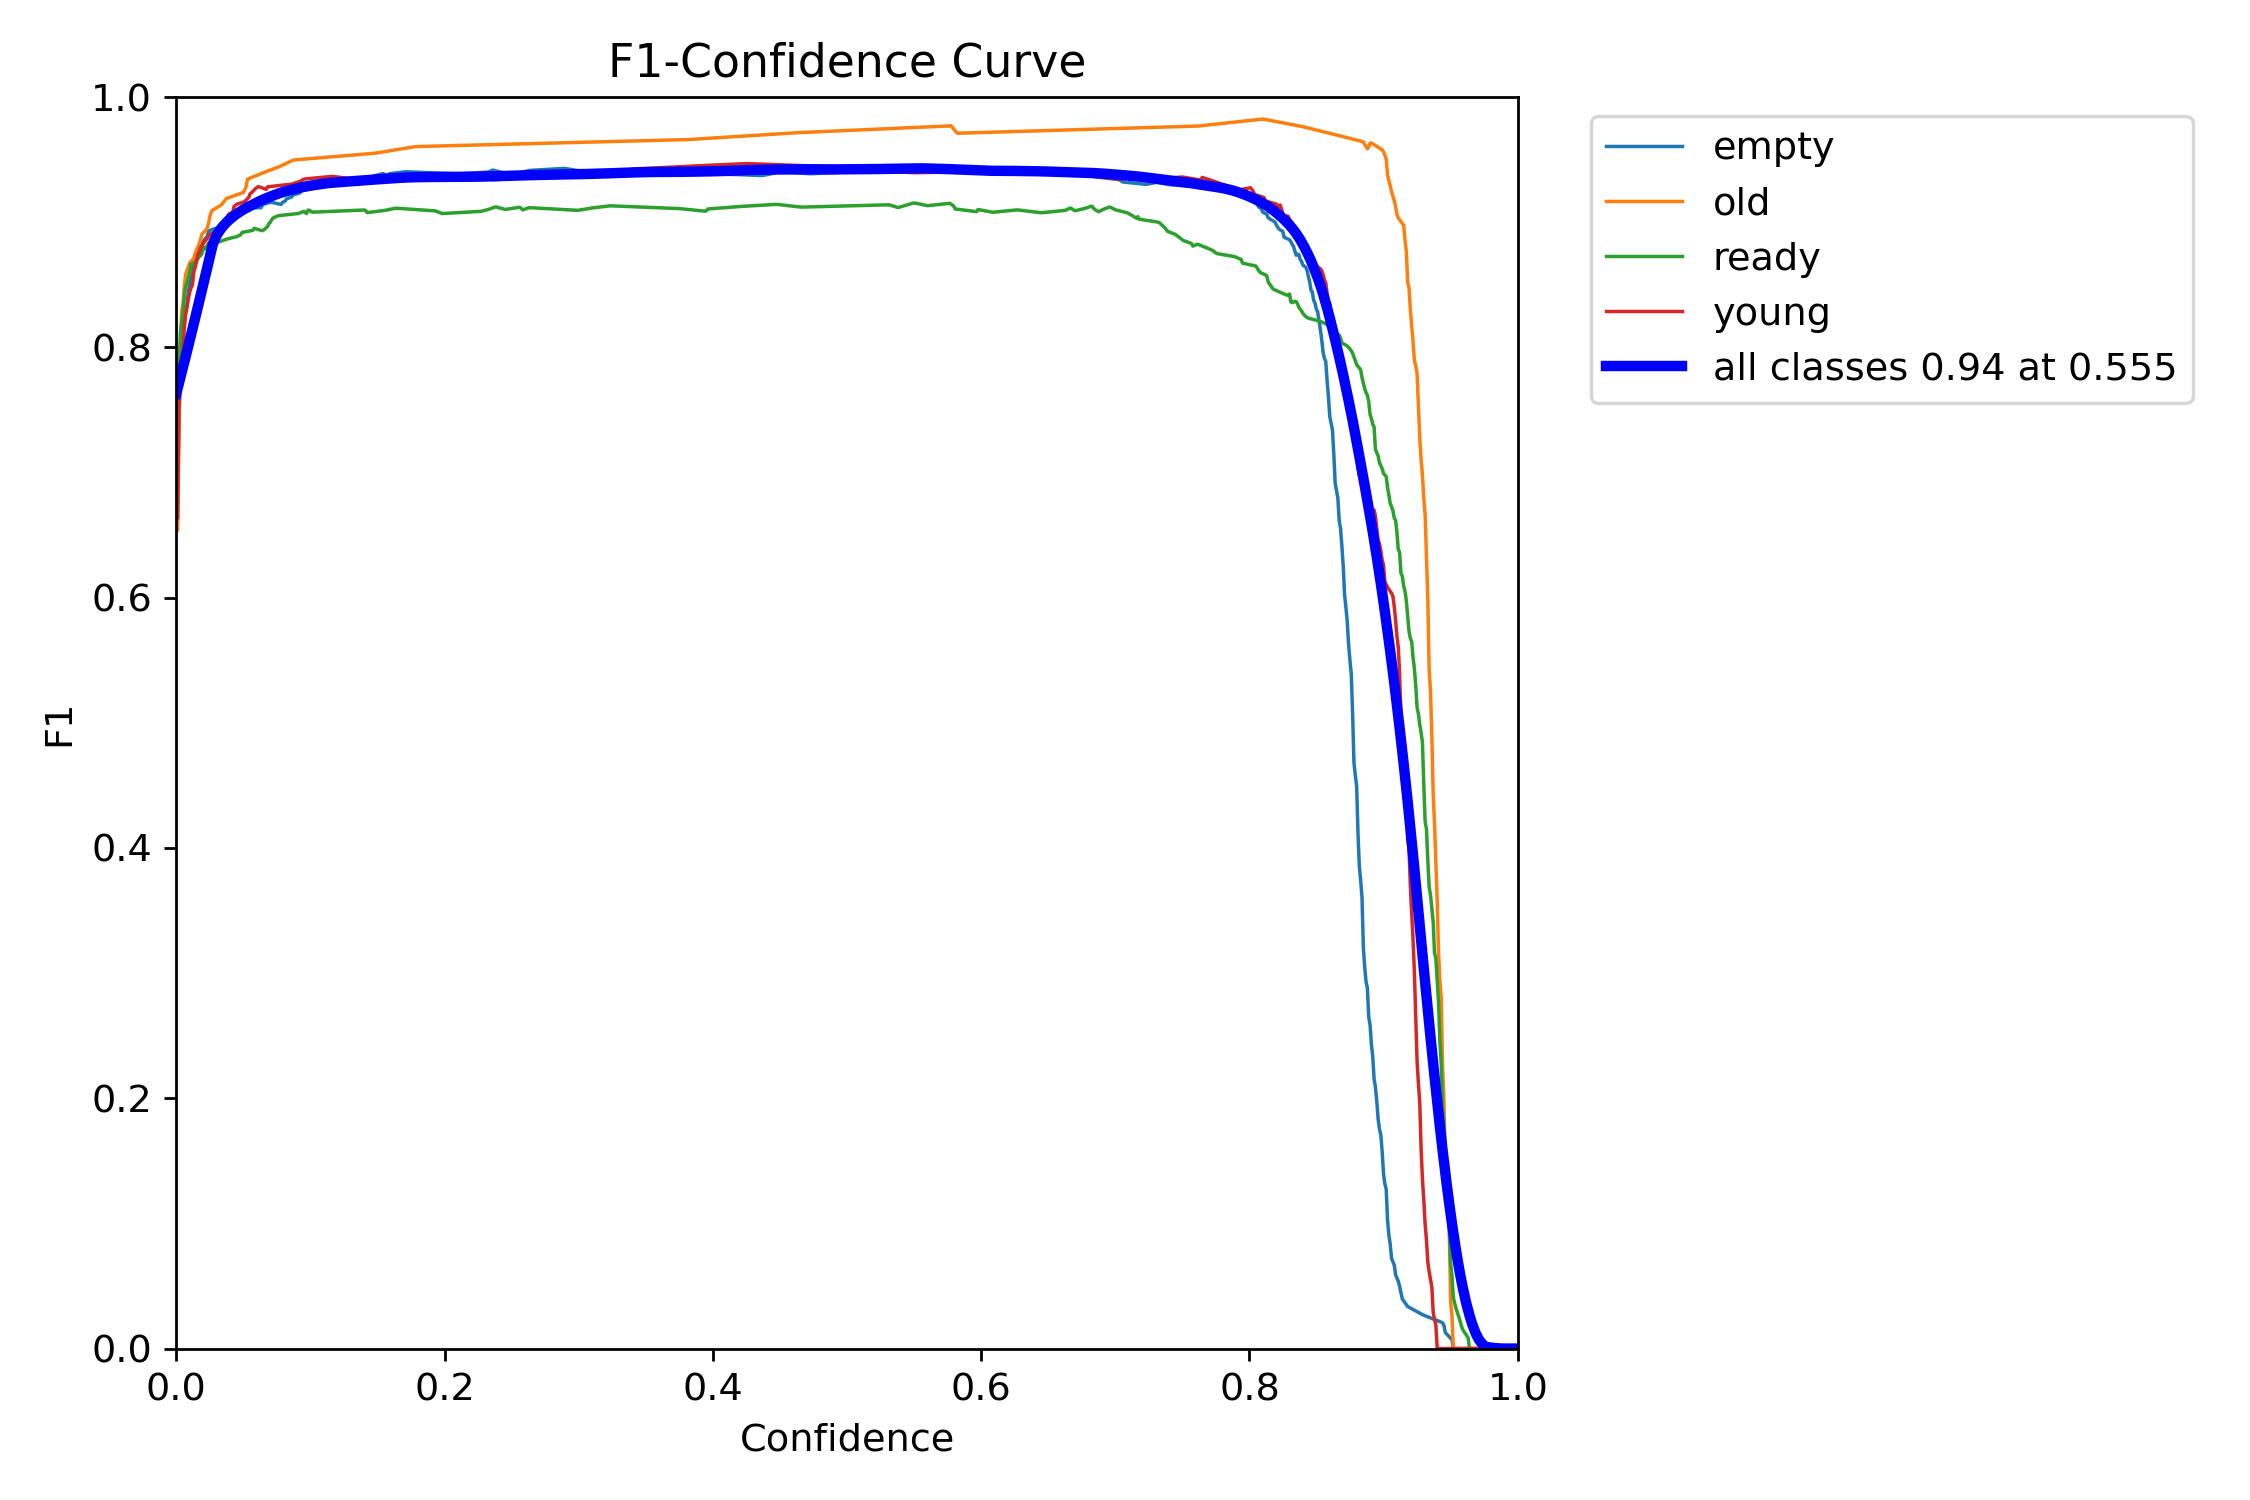
\includegraphics[width=0.95\linewidth]{images/F1_curve.png}
    \caption{Đường cong F1-score}
    \label{fig:training-result-f1}

    \end{subfigure}
    \caption{Kết quả huấn luyện}

    \label{fig:training-result}
\end{figure}

\begin{figure}[h]
    \centering
    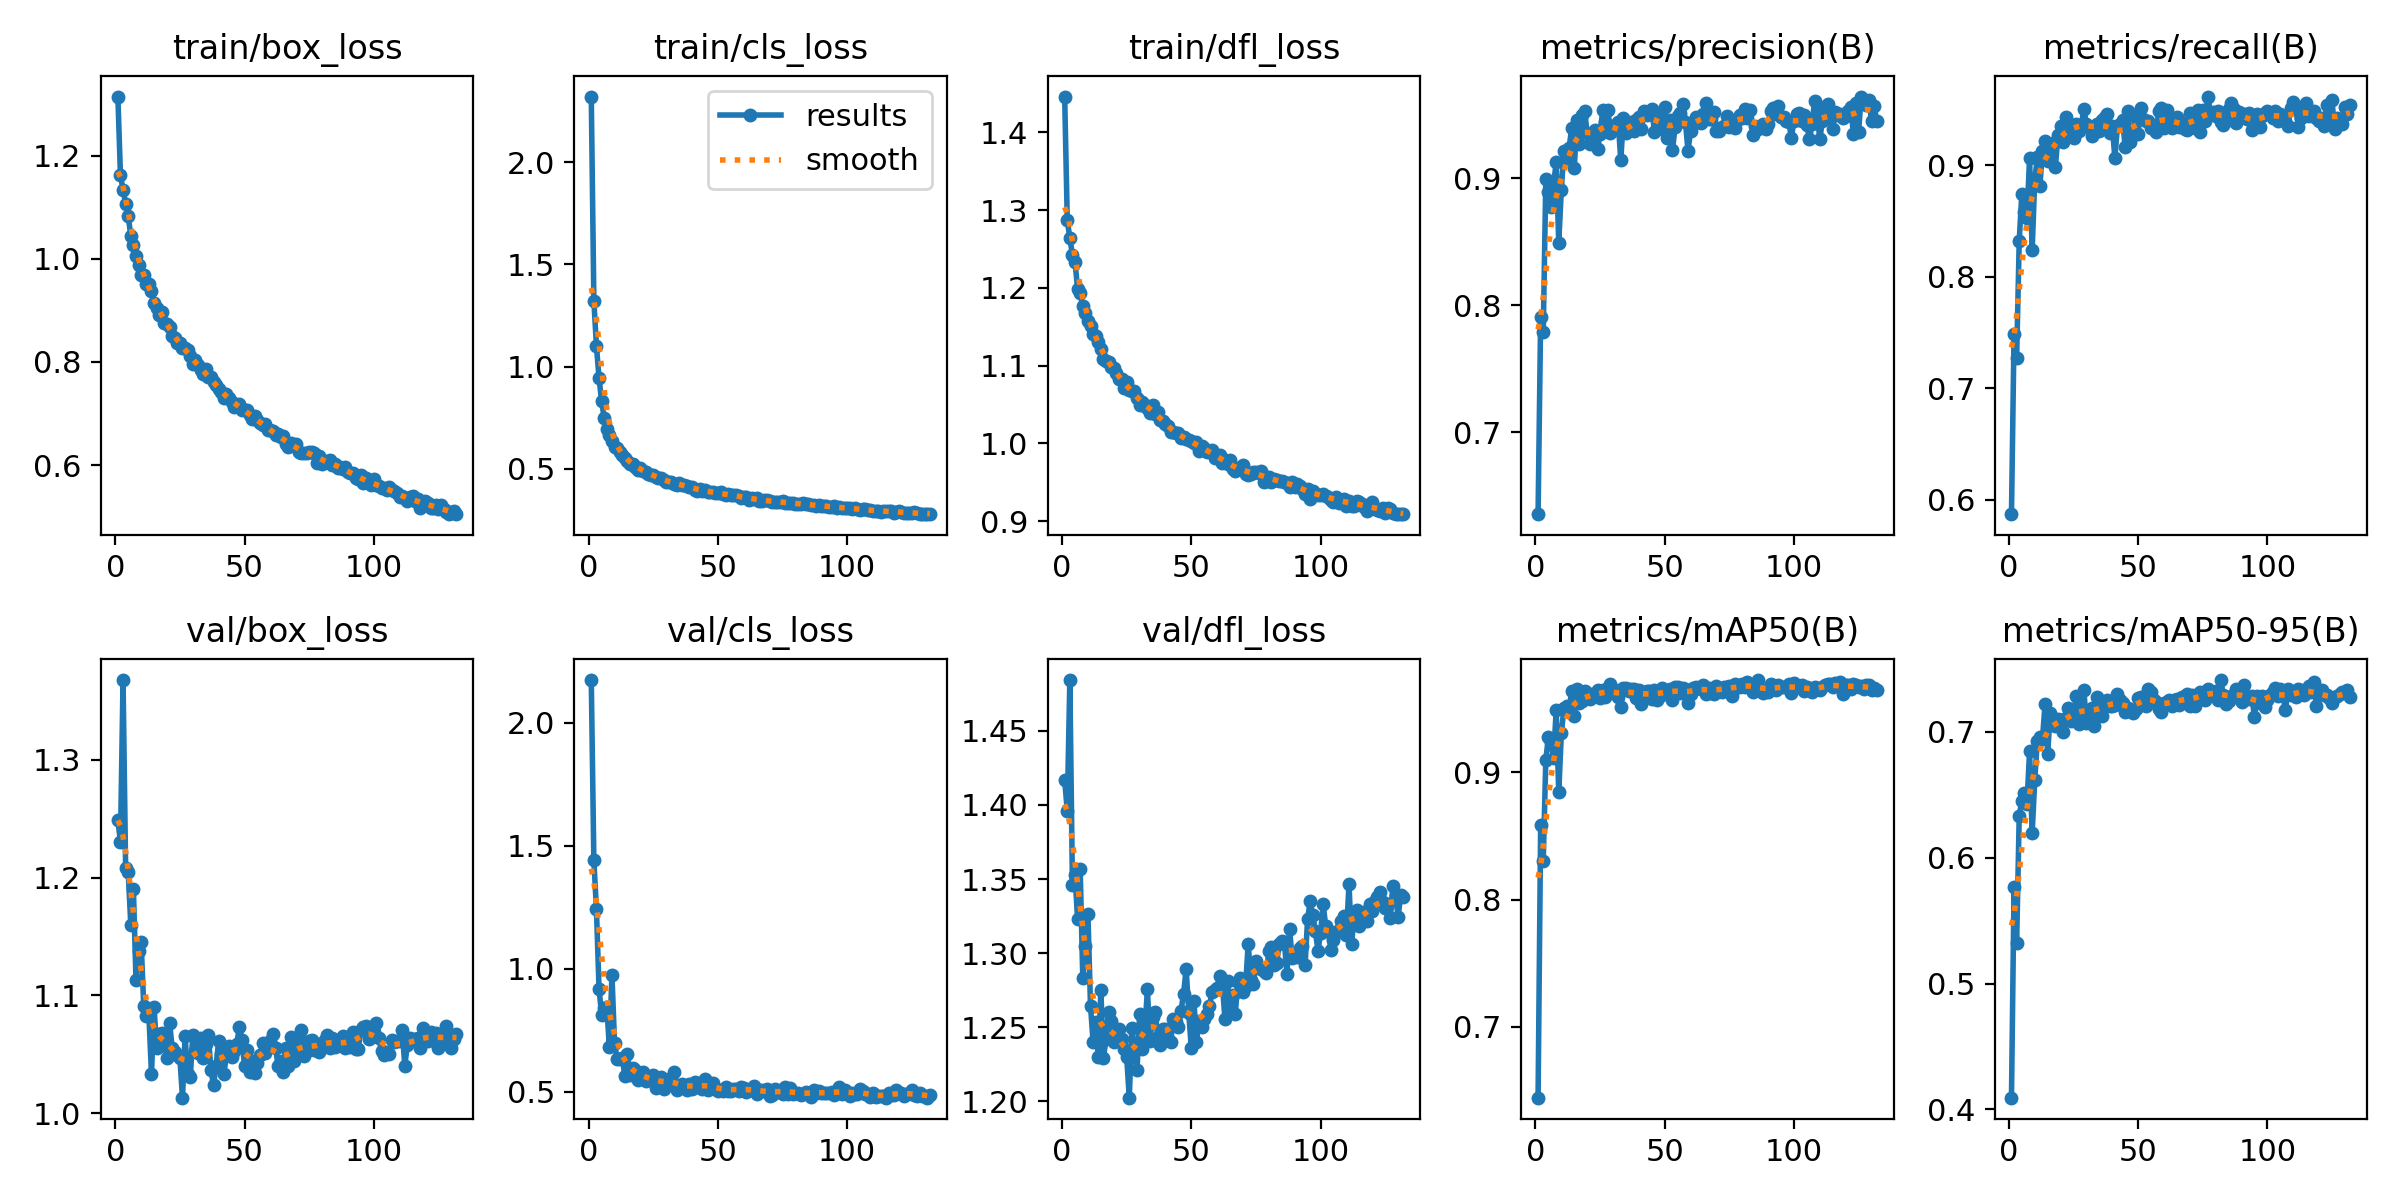
\includegraphics[width=0.85\linewidth]{images/results.png}
    \caption{Đồ thị mất mát}
    \label{fig:loss}
\end{figure}

Đồ thị \ref{fig:loss} cho thấy số lượng dữ liệu huấn luyện nhỏ nên gặp nhiều nhiều đỉnh trong đồ thị. Đồ thị mất mát cho việc phát hiện lớp "cls\_loss" có độ mịn, luôn ở ngưỡng thấp nên hoàn toàn phù hợp cho phát hiện trạng thái phát triển của nấm.

Đồ thị hàm mất mát cho hộp bao còn không ổn định, nhiều đỉnh cũng như gợn sóng. Điều này có thể nhận biết thông qua việc phát hiện hộp bao nhỏ hơn hoặc lớn hơn vật thể trong ảnh. Tuy nhiên, đối với bài toán phát hiện trạng thái phát triển của nấm, vị trí và kích thước hộp bao không cần độ chính xác tuyệt đối, vì vậy, mô hình huấn luyện này cũng phù hợp cho việc phát hiện trạng thái phát triển của nấm.

\begin{figure}[H]
	\centering
	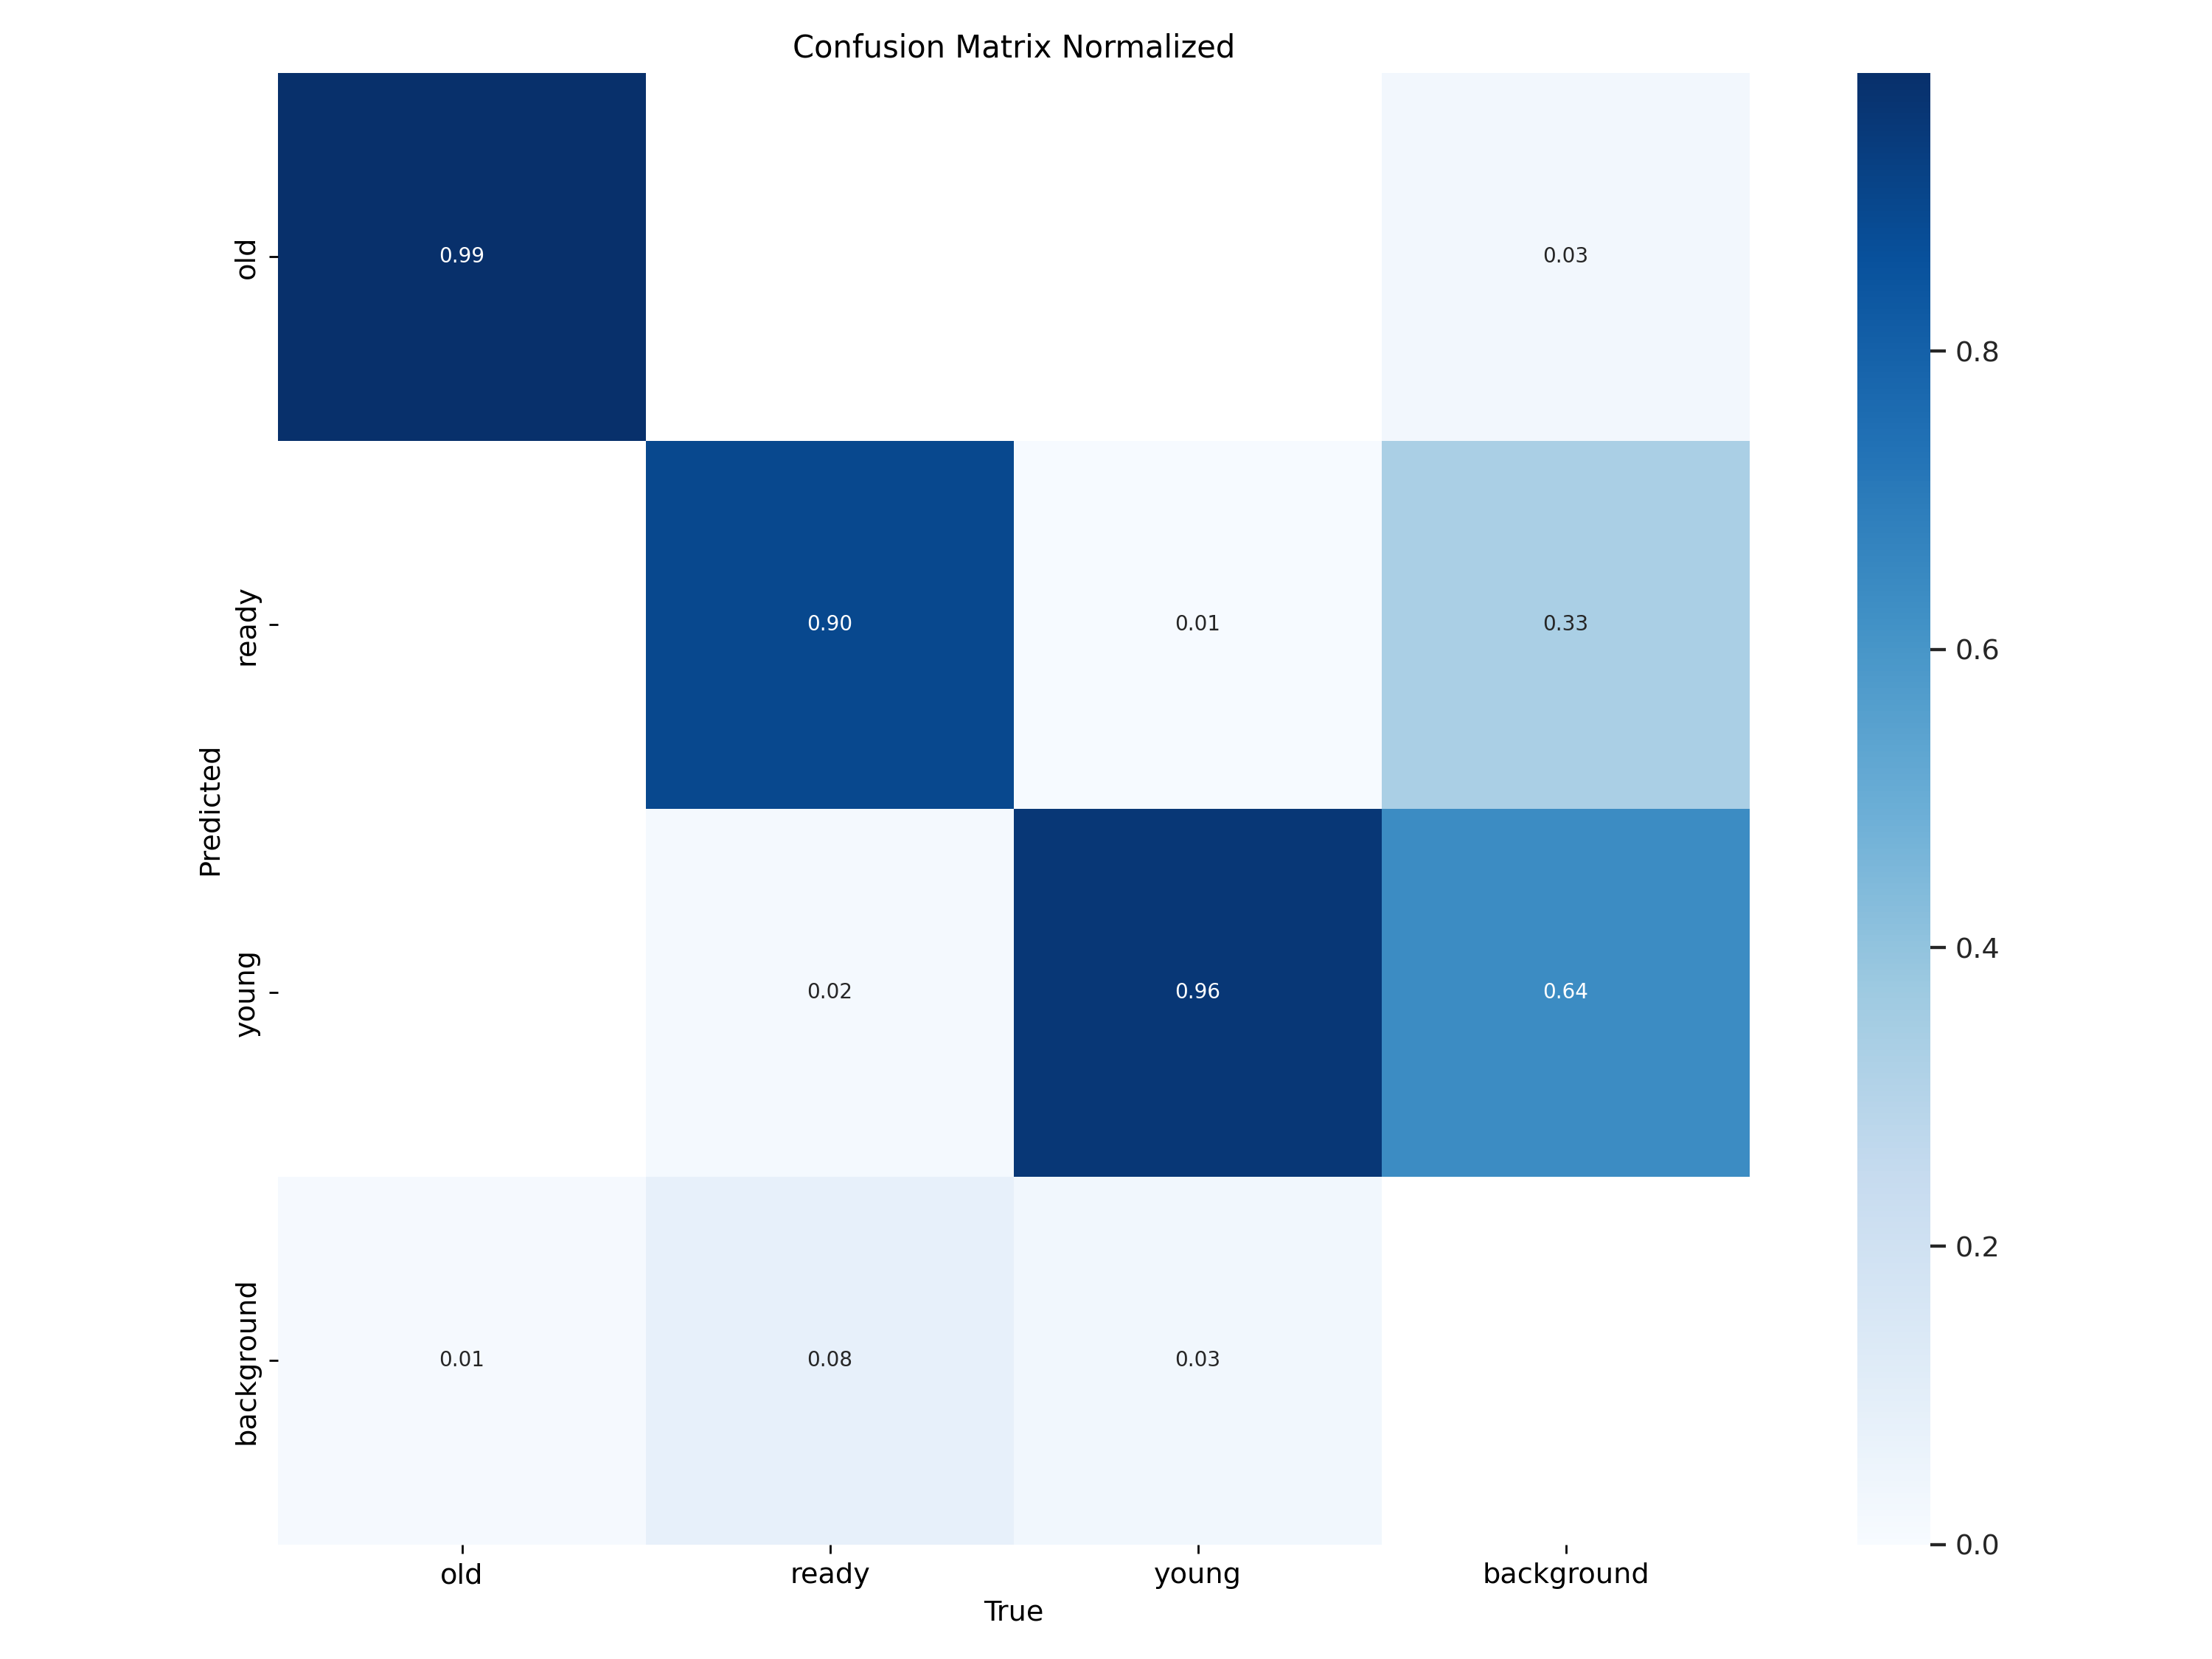
\includegraphics[width=0.8\linewidth]{images/confusion_matrix_normalized.png}
	\caption{Ma trận nhầm lẫn}
	\label{fig:confusion-matrix}
\end{figure}

Ma trận nhầm lẫn trong hình \ref{fig:confusion-matrix} cho thấy mô hình suy đoán chính xác ở mức cao, tuy nhiên nhiều trường hợp không suy đoán được trạng thái của nấm do tập dữ liệu còn nhỏ, chư bao quát hết các trường hợp trong quá trình huấn luyện. Vì vậy, tập dữ liệu cần bổ sung thêm.

\section{Tích hợp hệ thống}

\begin{figure}[h]
	\centering
	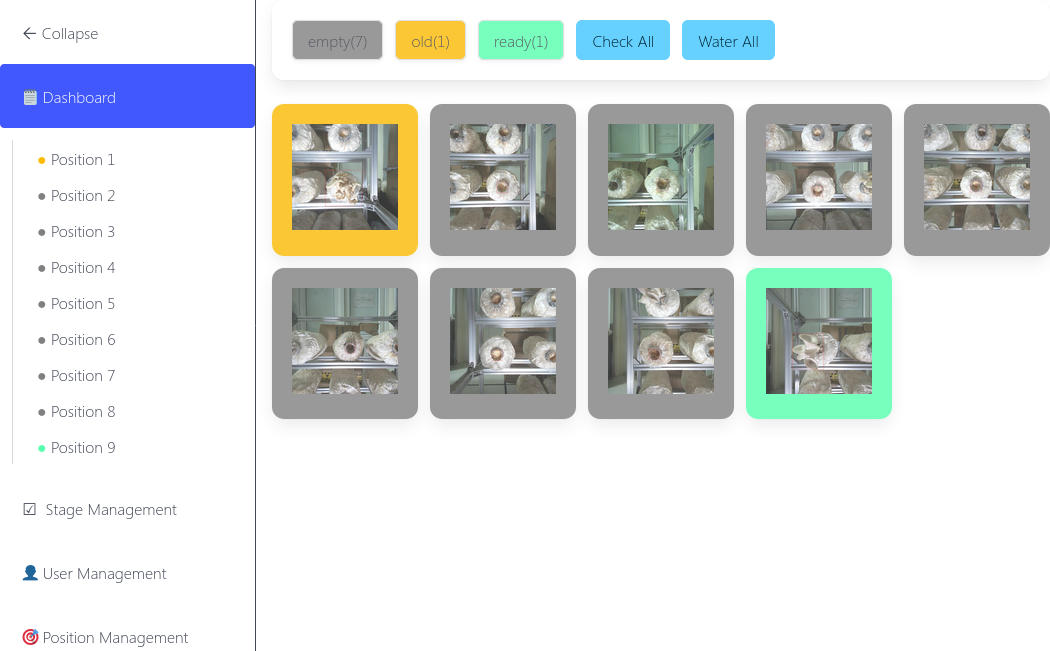
\includegraphics[width=0.8\linewidth]{images/ui-dashboard}
	\caption{Giao diện bảng điều khiển}
	\label{fig:ui-dashboard}
\end{figure}

\begin{figure}[H]
	\centering
	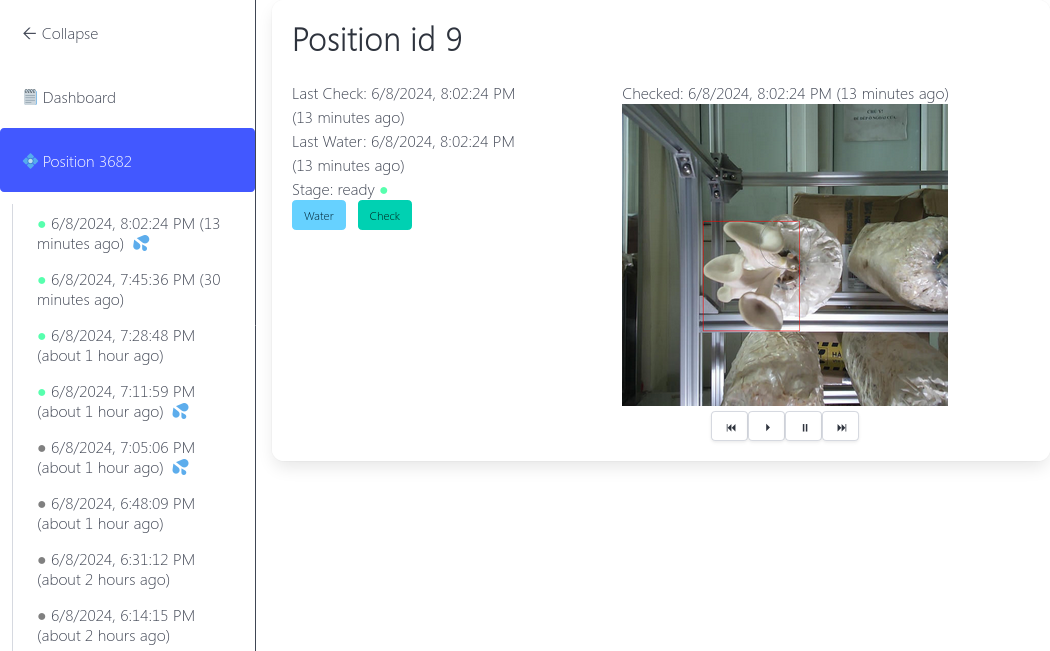
\includegraphics[width=0.8\linewidth]{images/ui-detail}
	\caption{Giao diện xem chi tiết vị trí}
	\label{fig:ui-detail}
\end{figure}

Sau khi huấn luyện, mô hình có thể được sử dụng trong hệ thống điều khiển. Giao diện người dùng hiển thị trạng thái hệ thống, hiển thị hình ảnh theo dõi và kết quả dự đoán trạng thái sinh trưởng chính xác. Màu của mỗi ô tương ứng với từng trạng thái sinh trưởng trống, non, trưởng thành, giá là xám, trắng, xanh lá, vàng như hình \ref{fig:ui-dashboard}.

Trong giao diện hiển thị chi tiết vị trí nấm, các trạng thái sinh trưởng cùng thời điểm chụp ảnh cũng được hiển thị rõ ràng. Ngoài ra, người dùng có thể xem lại quá trình sinh trưởng của nấm theo trình tự thời gian như hình \ref{fig:ui-detail}.

Qua thời gian thử nghiệm và tinh chỉnh, hệ thống có thể đưa ra kết quả kiểm tra tương đối chính xác cho từng vị trí nấm để có thể tưới nước theo từng giai đoạn phát triển của nấm. Các chức năng phụ như xem lại quá trình phát triển của nấm hoạt động đúng theo phương hướng đề ra. Tuy nhiên, một số ít thời điểm hệ thống không suy đoán được loại nấm tại vị trí chỉ định.

\section{Tổng kết chương}

Trong nửa đầu chương 3, đồ án mô tả các hoạt động của hệ thống sử dụng sơ đồ usecase, sơ đồ đối tượng và sơ đồ hợp tác mô tả hoạt động của người dùng với hệ thống, cấu trúc bên trong của hệ thống và hoạt động của các thành phần đó.

Tiếp theo, đồ án mô tả quá trình xây dựng tập dữ liệu huấn luyện và huấn luyện bao gồm:
\begin{itemize}
    \item Thu thập dữ liệu từ các nguồn khác nhau để đảm bảo độ đa dạng và đủ lớn cho quá trình huấn luyện.
    \item Tiền xử lý và chuẩn bị dữ liệu huấn luyện để đảm bảo chất lượng và độ tin cậy của dữ liệu.
    \item Huấn luyện mô hình và đánh giá hiệu suất của nó để đảm bảo rằng mô hình có khả năng phân loại các loại nấm một cách chính xác.
\end{itemize}

Cuối cùng, mô hình thị giác máy tính được tích hợp và chạy thử trong hệ thống với thành công bước đầu khi nhận diện trạng thái sinh trưởng của nấm thành công.
\chapter{XÂY DỰNG HỆ THỐNG TRỒNG NẤM SỬ DỤNG THỊ GIÁC MÁY TÍNH}
\section{Xây dựng hệ thống theo dõi và chăm sóc nấm}
\subsection{Sơ đồ triển khai}

Hệ thống bao gồm thiết bị ghi hình, thiết bị điều khiển môi trường, thiết bị điều khiển trung tâm và giao diện người dùng.

\begin{figure}[h]
    \centering
    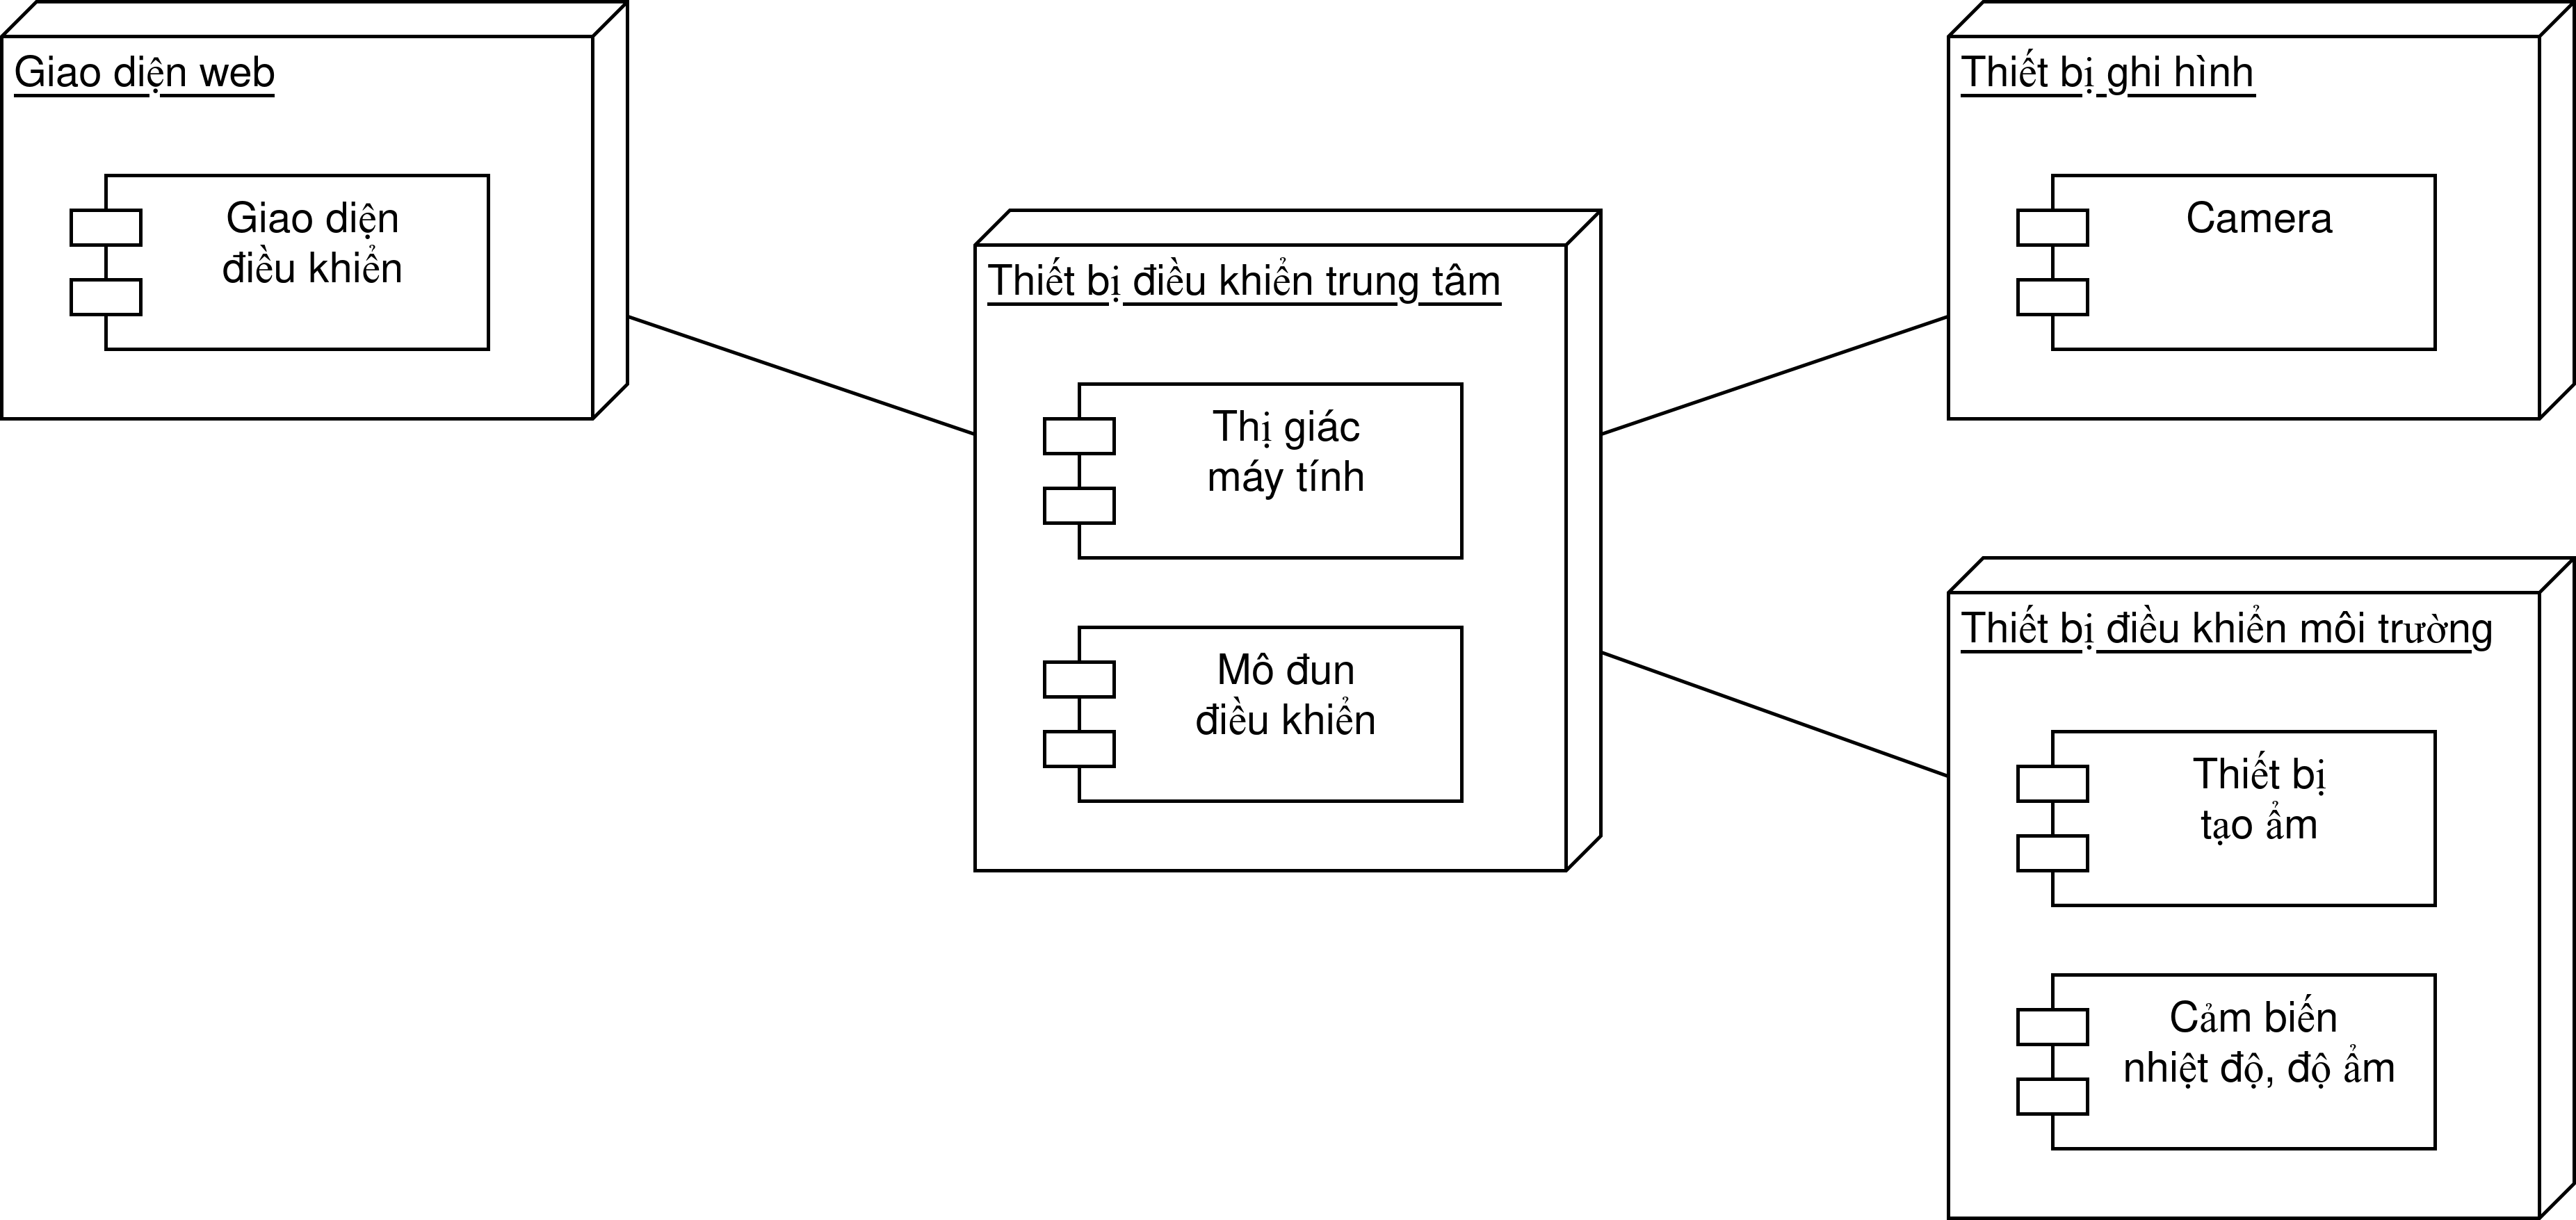
\includegraphics[width=0.75\linewidth]{images/deploy.png}
    \caption{Sơ đồ triển khai hệ thống}
    \label{fig:deploy}
\end{figure}

\subsection{Thiết kế phần mềm}

Phần mềm được chia thành các mô đun nhỏ thực hiện các chức năng khác nhau (Hình \ref{fig:software-component}).

\begin{itemize}
    \item Mô đun nhận hình ảnh thực hiện lấy hình ảnh từ Camera IP về thiết bị.
    \item Mô đun xử lý hình ảnh thực hiện phân tích hình ảnh bằng thị giác máy tính, giúp phát hiện và đưa ra vị trí nấm.
    \item Mô đun điều khiển tưới nước thực hiện bật tắt thiết bị tạo ẩm.
    \item Mô đun giao tiếp tạo diao diện kết nối giữa người dùng và mô đun điều khiển.
    \item Mô đun điều khiển thực hiện ghép nối các thành phần và gọi các mô đun tương ứng.
    \item Giao diện hiển thị hiển thị trạng thái hệ thống cho người quản lý.
\end{itemize}

\begin{figure}
    \centering
    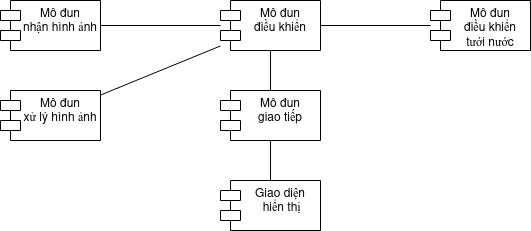
\includegraphics[width=0.75\linewidth]{images/software-component.png}
    \caption{Các thành phần phần mềm}
    \label{fig:software-component}
\end{figure}

\begin{figure}
    \centering
    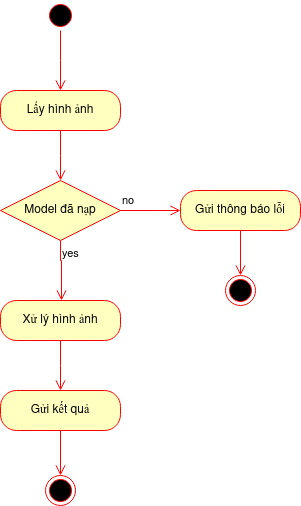
\includegraphics[width=0.55\linewidth]{images/vision-actvity.png}
    \caption{Biểu đồ hoạt động tác vụ phát hiện nấm}
    \label{fig:vision-activity}
\end{figure}


\begin{figure}[H]
    \centering
    \includegraphics[width=0.55\linewidth]{images/ui-activity.png}
    \caption{Biểu đồ hoạt động giao diện người dùng}
    \label{fig:ui-activity}
\end{figure}

Việc chia nhỏ các tác vụ và thực hiện chúng song song có thể tối ưu hóa hiệu suất của ứng dụng. Khi các tác vụ không phụ thuộc vào nhau và có thể được thực hiện độc lập, ta có thể thực hiện chúng cùng một lúc trên nhiều luồng hoặc tiến trình, tận dụng được tài nguyên phần cứng và giảm thời gian thực thi.

Phần mềm được lập trình trên ngôn ngữ Rust, giúp việc lập trình song song trở nên đơn giản và an toàn hơn \cite{rust2022}. Ngoài ra, việc sử dụng ngôn ngữ lập trình biên dịch cùng các chế độ tối ưu hóa cũng giúp chương trình có hiệu suất cao hơn so với các ngôn ngữ thông dịch như Python.

\section{Xây dựng tập dữ liệu và huấn luyện mô hình}

\subsection{Thu thập dữ liệu}

Ngoài dữ liệu hình ảnh thu được trong thực tế trồng nấm, nguồn ảnh huấn luyện có thể thu thập từ nguồn mạng xã hội.

Roboflow là một nền tảng hỗ trợ tốt cho việc chuẩn bị dữ liệu huấn luyện. Dữ liệu huấn luyện có thể được tải lên Roboflow dưới dạng ảnh hoặc dạng video sau đó chuyển thành từng khung hình.


\subsection{Tiền xử lý và chuẩn bị dữ liệu huấn luyện}

Sau khi chuẩn bị dữ liệu huấn luyện, thực hiện gán nhãn cho từng vật thể (Hình \ref{fig:labeling-interface}).

\begin{figure}[H]]
    \centering
    \includegraphics[width=0.85\linewidth]{images/image-labeling.png}
    \caption{Giao diện gán nhãn cho vật thể}
    \label{fig:labeling-interface}
\end{figure}

Nấm non có thân mọc thẳng về các phía, kích thước tai nấm không lớn hơn thân đáng kể (Hình \ref{fig:young}).

\begin{figure}[H]
    \centering
        \begin{subfigure}{.5\textwidth}
        \includegraphics[width=0.8\linewidth]{images/young2.png}
    \end{subfigure}%
    \begin{subfigure}{.5\textwidth}
        \includegraphics[width=0.8\linewidth]{images/young3.png}
    \end{subfigure}
    \caption{Hình ảnh nấm non}
    \label{fig:young}
\end{figure}

Nấm trưởng thành có tai nấm phát triển, thân nấm uốn cong lên phía trên (Hình \ref{fig:ready}).

\begin{figure}[H]
    \centering
        \begin{subfigure}{.5\textwidth}
        \includegraphics[width=0.8\linewidth]{images/ready1.png}
    \end{subfigure}%
    \begin{subfigure}{.5\textwidth}
        \includegraphics[width=0.8\linewidth]{images/ready3.png}
    \end{subfigure}
    \caption{Hình ảnh nấm trưởng thành, có thể thu hoạch}
    \label{fig:ready}
\end{figure}

Nấm già tai nấm phát triển to có thể bị xoăn lại và chuyển sang màu vàng., thân nấm nhỏ (Hình \ref{fig:old}).
\begin{figure}[H]
    \centering
    \begin{subfigure}{.5\textwidth}
        \includegraphics[width=0.85\linewidth]{images/old1.png}
    \end{subfigure}%
    \begin{subfigure}{.5\textwidth}
        \includegraphics[width=0.85\linewidth]{images/old3.png}
    \end{subfigure}
    \caption{Hình ảnh nấm già}
    \label{fig:old}
\end{figure}

Dữ liệu huấn luyện sau khi chuẩn bị đầy đủ có thể được tải về và đưa vào huấn luyện (Hình \ref{fig:export-dataset}).
\begin{figure}[H]
    \centering
    \includegraphics[width=0.85\linewidth]{images/export-dataset.png}
    \caption{Xuất tập dữ liệu huấn luyện}
    \label{fig:export-dataset}
\end{figure}

Tổng số nhãn gán cho ảnh bao gồm khoảng 2500 nấm non, 2500 nấm trưởng thành và 750 nấm già (Hình \ref{fig:instances-graph}).
\begin{figure}
    \centering
    \includegraphics[width=0.55\linewidth]{images/instances-graph.png}
    \caption{Thống kê số lượng nhãn}
    \label{fig:instances-graph}
\end{figure}


Tổng số ảnh chuẩn bị cho huấn luyện là 753 ảnh. Sau quá trình tăng cường dữ liệu nghiêng ảnh và thêm nhiễu, số ảnh phục vụ huấn luyện là 1809 bao gồm 1586 ảnh huấn luyện, 152 ảnh giám sát và 71 ảnh kiểm thử.


\subsection{Huấn luyện và đánh giá hiệu suất mô hình}

Mô hình thị giác máy tính có thể được thực hiện nhờ google colab (Hình \ref{fig:colab-ui}.

\begin{figure}[h]
    \centering
    \includegraphics[width=0.85\linewidth]{images/colab-inteface.png}
    \caption{Giao diện Google Colab và mã nguồn}
    \label{fig:colab-ui}
\end{figure}

Nhập các thư viện YOLOv8:
\begin{lstlisting}
    %pip install ultralytics
\end{lstlisting}

Bắt đầu huấn luyện với các tham số:

\begin{itemize}
    \item train: Tác vụ huấn luyện
    \item data: Nơi lưu trữ tập dữ liệu tải từ Roboflow
    \item model: Kích thước model sử dụng, X là lớn nhất, s là nhỏ, n là nhỏ nhất. Do dữ liệu huấn luyện có số lượng nhỏ nên sử dụng n để tránh overfiting.
    \item epochs: Số vòng huấn luyện. Thử từ 50 epoch do số lượng dữ liệu huấn luyện nhỏ.
\end{itemize}
\begin{lstlisting}
!yolo train data=data.yaml model=yolov8n.pt epochs=50 lr0=0.01
\end{lstlisting}

Chuyển mô hình huấn luyện được về dạng safetensors và chỉnh sửa mô hình để chạy trên Candle:
\begin{lstlisting}[language=python]
import torch
from safetensors.torch import load_file
from safetensors.torch import save_file

def rename(name: str):
    name = name.replace("model.0.", "net.b1.0.")
    name = name.replace("model.1.", "net.b1.1.")
    name = name.replace("model.2.m.", "net.b2.0.bottleneck.")
    name = name.replace("model.2.", "net.b2.0.")
    name = name.replace("model.3.", "net.b2.1.")
    name = name.replace("model.3.", "net.b2.1.")
    name = name.replace("model.4.m.", "net.b2.2.bottleneck.")
    name = name.replace("model.4.", "net.b2.2.")
    name = name.replace("model.5.", "net.b3.0.")
    name = name.replace("model.6.m.", "net.b3.1.bottleneck.")
    name = name.replace("model.6.", "net.b3.1.")
    name = name.replace("model.7.", "net.b4.0.")
    name = name.replace("model.8.m.", "net.b4.1.bottleneck.")
    name = name.replace("model.8.", "net.b4.1.")
    name = name.replace("model.9.", "net.b5.0.")
    name = name.replace("model.12.m.", "fpn.n1.bottleneck.")
    name = name.replace("model.12.", "fpn.n1.")
    name = name.replace("model.15.m.", "fpn.n2.bottleneck.")
    name = name.replace("model.15.", "fpn.n2.")
    name = name.replace("model.16.", "fpn.n3.")
    name = name.replace("model.18.m.", "fpn.n4.bottleneck.")
    name = name.replace("model.18.", "fpn.n4.")
    name = name.replace("model.19.", "fpn.n5.")
    name = name.replace("model.21.m.", "fpn.n6.bottleneck.")
    name = name.replace("model.21.", "fpn.n6.")
    name = name.replace("model.22.", "head.")
    return name

data = torch.load("runs/detect/train5/weights/last.pt")
tensors = data['model'].state_dict().items()
tensors = dict(tensors)
tensors = {rename(k): t for k, t in tensors.items()}
print(data["model"])
save_file(tensors, "/runs/detect/train5/weights/last.safetensors")
for k, v in tensors.items():
    print(str(k), v.shape)
\end{lstlisting}

Từ hình \ref{fig:training-result-f1}, mô hình đưa ra kết quả chính xác nhất với hệ số tự tin từ 20\% đến 70\%, hệ số tự tin càng cao càng đưa ra kết quả chính xác trong hình \ref{fig:training-result-p} và tỉ lệ phát hiện đúng vật thể giảm rõ rệt khi hệ số tự tin lớn hơn 70\% (Hình \ref{fig:training-result-r}).

\begin{figure}
    \centering
    \begin{subfigure}{.5\textwidth}
        \includegraphics[width=0.95\linewidth]{images/P_curve.png}
    \caption{Đường cong Precision}
    \label{fig:training-result-p}

    \end{subfigure}%
    \begin{subfigure}{.5\textwidth}
        \includegraphics[width=0.95\linewidth]{images/R_curve.png}
    \caption{Đường cong Recall}
    \label{fig:training-result-r}
    \end{subfigure}
    \begin{subfigure}{.5\textwidth}
        \includegraphics[width=0.95\linewidth]{images/F1_curve.png}
    \caption{Đường cong F1-score}
    \label{fig:training-result-f1}

    \end{subfigure}
    \caption{Kết quả huấn luyện}

    \label{fig:training-result}
\end{figure}

\begin{figure}[h]
    \centering
    \includegraphics[width=0.85\linewidth]{images/results.png}
    \caption{Đồ thị mất mát}
    \label{fig:loss}
\end{figure}

Đồ thị \ref{fig:loss} cho thấy số lượng dữ liệu huấn luyện nhỏ nên gặp nhiều nhiều đỉnh trong đồ thị. Sau khoảng 40 vòng huấn luyện, đồ thị mất mát cho tác vụ xác định vị trí vẫn đang đi xuống với góc nghiêng nhỏ nên còn bị underfitting. Tuy nhiên, đồ thị mất mất cho tác vụ phân lớp gần như nằm ngang nên không bị overfitting hay underfitting. 

Ma trận thu (Hình \ref{fig:confusion-matrix}) cho thấy mô hình đoán nhận khá chính xác, tuy nhiên nhiều trường hợp không đoán nhận được nấm non do nhiều hình ảnh nấm quá non bị thiếu độ chi tiết, cần chỉnh sửa thêm.


\begin{figure}[H]
    \centering
    \includegraphics[width=0.85\linewidth]{images/confusion_matrix_normalized.png}
    \caption{Ma trận thu}
    \label{fig:confusion-matrix}
\end{figure}

\section{Tích hợp và tinh chỉnh hệ thống}
Sau khi huấn luyện, mô hình có thể được sử dụng trong hệ thống. 



\begin{table}[H]
\centering
\caption{Thông số chạy chương trình}
\label{tab:run-command}
\begin{tabular}{|l|l|l|}
\hline
\textbf{Thuộc tính} & \textbf{Giá trị mặc định} & \textbf{Mô tả}                     \\ \hline
--port              & {[}default: 8080{]}       & Cổng cho api                       \\ \hline
--model-path        &                           & Đường dẫn tới mô hình              \\ \hline
--model-size        & {[}default: m{]}          & Kích thước mô hình \\ \hline
--num-classes       & {[}default: 1{]}          & Số lớp nhận diện bởi mô            \\ \hline
--store-path        & {[}default: ./images{]}   & Đường dẫn lưu ảnh                  \\ \hline
--camera-device     &                           & Thiết bị camera                    \\ \hline
--snapshot-url      &                           & Đường dẫn lấy hình ảnh camera      \\ \hline
--stream-url        & {[}default: /video{]}     & Đường dẫn video camera             \\ \hline
--pump-pin          &                           & Chân gpio kết nối bơm              \\ \hline
--pump-on           & {[}default: 1{]}          & Thời gian bơm bật                  \\ \hline
--pump-off          & {[}default: 1{]}          & Thời gian bơm tắt                  \\ \hline
\end{tabular}
\end{table}

Giao diện người dùng hiển thị trạng thái hệ thống, hiển thị hình ảnh theo dõi và hộp bao tương ứng với kết quả tương đối chính xác với cả hộp bao và trạng thái sinh trưởng (Hình \ref{fig:user-interface}).
\begin{figure}[H]
    \centering
    \includegraphics[width=0.75\linewidth]{images/user-interface.png}
    \caption{Giao diện nhận diện ảnh nấm}
    \label{fig:user-interface}
\end{figure}


\section{Tổng kết chương}

Trong chương 3, phần "Xây dựng hệ thống theo dõi và chăm sóc nấm" bao gồm sơ đồ triển khai hệ thống, bao gồm liên kết giữa các thành phần với nhau. 

Tiếp theo, phần "Xây dựng tập dữ liệu và huấn luyện mô hình" là quá trình xây dựng tập dữ liệu huấn luyện bao gồm:
\begin{itemize}
    \item Thu thập dữ liệu từ các nguồn khác nhau để đảm bảo độ đa dạng và đủ lớn cho quá trình huấn luyện.
    \item Tiền xử lý và chuẩn bị dữ liệu huấn luyện để đảm bảo chất lượng và độ tin cậy của dữ liệu.
    \item Huấn luyện mô hình và đánh giá hiệu suất của nó để đảm bảo rằng mô hình có khả năng phân loại các loại nấm một cách chính xác.
\end{itemize}

Cuối cùng, mô hình thị giác máy tính được tích hợp và chạy thử trong hệ thống với thành công bước đầu khi nhận diện trạng thái sinh trưởng của nấm thành công.
\renewcommand\bibname{TÀI LIỆU THAM KHẢO}

\bibliographystyle{plain}

\bibliography{essential/refs}

%\cleardoublepage
\phantomsection
\chapter*{Phụ lục}
\addcontentsline{toc}{section}{PHỤ LỤC}
\pagenumbering{gobble}
\end{document}
